%%
%%  Department of Electrical, Electronic and Computer Engineering.
%%  EPR400/2 Final Report - Main File.
%%  Copyright (C) 2011-2021 University of Pretoria.
%%

\documentclass{epr400}

%% Additional packages
\usepackage[hyphens]{url} % Allow line breaks in bibtex URL\
\usepackage{subcaption}

%% Additional commands
\newcommand{\matr}[1]{\bm{#1}}
\newcommand{\vect}[1]{\bm{#1}}

%% EDIT: Replace the following with your information.
\eprtitle{3D cube-world construction robot}
\eprcode{EPR402}
\eprcandidatename{C.H. Conroy}
\eprstudentnumber{18072918}
\eprdate{November 2021}
\eprsupervisor{Mr. H. Grobler}
\eprcopynum{Electronic copy}

\begin{document}

%% Generate the required title page.
\maketitlepage

%% --- PART 1 ------------------------------------------------------------

\pagestyle{plain}
\pagenumbering{roman}

\eprsec{Part 1. Preamble}

\vspace*{0.5cm}

%% Import the required preamble pages.
%%
%%  Department of Electrical, Electronic and Computer Engineering.
%%  EPR400/2 Final Report - Preamble.
%%  Copyright (C) 2011-2021 University of Pretoria.
%%

This report describes work that I did in my final year project, developing a robotic system to construct arbitrary 3D shapes using small cubes.
\\[2ex]
\textit{Project proposal and technical documentation} \newline
This main report contains an unaltered copy of the approved Project Proposal (as Part 2 of the report).

Technical documentation appears in Part 4 (Appendix).

All the code that I developed appears as a separate submission on the AMS.
\\[2ex]
\textit{Project history} \newline
This project makes use of existing algorithms in the traditional computer vision domain relating to object detection and 3D object localisation as a basis for the computer vision project component. However, the adaptation and implementation of these algorithms in this project is my own work. This also applies to the algorithms used to create the coordinate system transformation matrices in the OpenGL 3D shape render component. A number of basic image processing and camera calibration methods were used from the OpenCV library. Furthermore, the C++ QT framework was used as the basis for the PC-based software component. Where other authors' work has been used, it has been cited appropriately, and the rest of the work reported on here, is entirely my own.
\\[2ex]
\textit{Language editing} \newline
This document has been language edited by a knowledgeable person. By submitting this document in its present form, I declare that this is the written material that I wish to be examined on.

My language editor was Christopher Henry Conroy.

\vspace*{1.2cm}

\begin{tabular}{lp{1cm}ll}
\makebox[3in]{\hrulefill}  &  & \makebox[1.5in]{\hrulefill} \\
\textit{Language editor signature}  &  & \textit{Date}
\end{tabular}

\vspace*{0.5cm}

\textit{Declaration}
\\[2ex]
I, Christopher Henry Conroy understand what plagiarism is and have carefully studied the plagiarism policy of the University. I hereby declare that all the work described in this report is my own, except where explicitly indicated otherwise. Although I may have discussed the design and investigation with my study leader, fellow students or consulted various books, articles or the Internet, the design/investigative work is my own. I have mastered the design and I have made all the required calculations in my lab book (and/or they are reflected in this report) to authenticate this. I am not presenting a complete solution of someone else.

Wherever I have used information from other sources, I have given credit by proper and complete referencing of the source material so that it can be clearly discerned what is my own work and what was quoted from other sources. I acknowledge that failure to comply with the instructions regarding referencing will be regarded as plagiarism.  If there is any doubt about the authenticity of my work, I am willing to attend an oral ancillary examination/evaluation about the work.

I certify that the Project Proposal appearing as the Introduction section of the report is a verbatim copy of the approved Project Proposal.

\vspace{1.2cm}

\begin{tabular}{lp{1cm}ll}
\makebox[3in]{\hrulefill}  &  & \makebox[1.5in]{\hrulefill} \\
\eprthecandidatename       &  & Date
\end{tabular}

%% End of File.


\newpage

%% Add the Table of Contents.
\tableofcontents
\thispagestyle{empty}
\newpage

%% Import the required abbreviation pages.
%%
%%  Department of Electrical, Electronic and Computer Engineering.
%%  EPR400/2 Final Report - Abbreviations.
%%  Copyright (C) 2011-2021 University of Pretoria.
%%

\section*{LIST OF ABBREVIATIONS}

\begin{tabular}{p{3cm}l}
%  \textbf{AWGN}         &  Additive white Gaussian noise \\
%  \textbf{BER}          &  Bit error rate \\
%  \textbf{BPSK}         &  Bipolar phase shift keying \\
%  \textbf{DSP}          &  Digital signal processor \\
%  \textbf{GSM}          &  Global System for Mobile communications \\
%  \textbf{SNR}          &  Signal-to-noise-ratio  \\
  
  	\textbf{API}			& Application programming interface \\
  	\textbf{BRIEF}			& Binary robust independent elementary features \\
	\textbf{CNN} 			& Convolutional neural network \\
	\textbf{DLT}			& Direct Linear Transform \\
	\textbf{DoF}			& Degrees of Freedom \\
	\textbf{EP\textit{n}P}	& Efficient P\textit{n}P \\
	\textbf{FAST}			& Features from accelerated segment test \\
	\textbf{GUI}			& Graphical user interface \\
	\textbf{ORB}			& Oriented FAST and rotated BRIEF \\
	\textbf{PCB}			& Printed circuit board \\
	\textbf{P\textit{n}P}	& Perspective-\textit{n}-Point \\
	\textbf{RGB}			& Red, green and blue \\
	\textbf{RGBD}			& Red, green, blue and depth \\
	\textbf{ROI}			& Region of interest \\
	\textbf{SIFT}			& Scale-invariant feature transform \\
	\textbf{SURF}			& Speeded-up robust features \\
	\textbf{ToF}			& Time-of-flight \\
	

\end{tabular}

%% End of File.
\newpage

%% --- PART 2 ------------------------------------------------------------

\eprsec{Part 2. Project definition: approved Project Proposal}

This section contains the problem identification in the form of the complete approved Project Proposal, unaltered from the final approved version that appears on the AMS.

\newpage

%% Import the approved project proposal
% 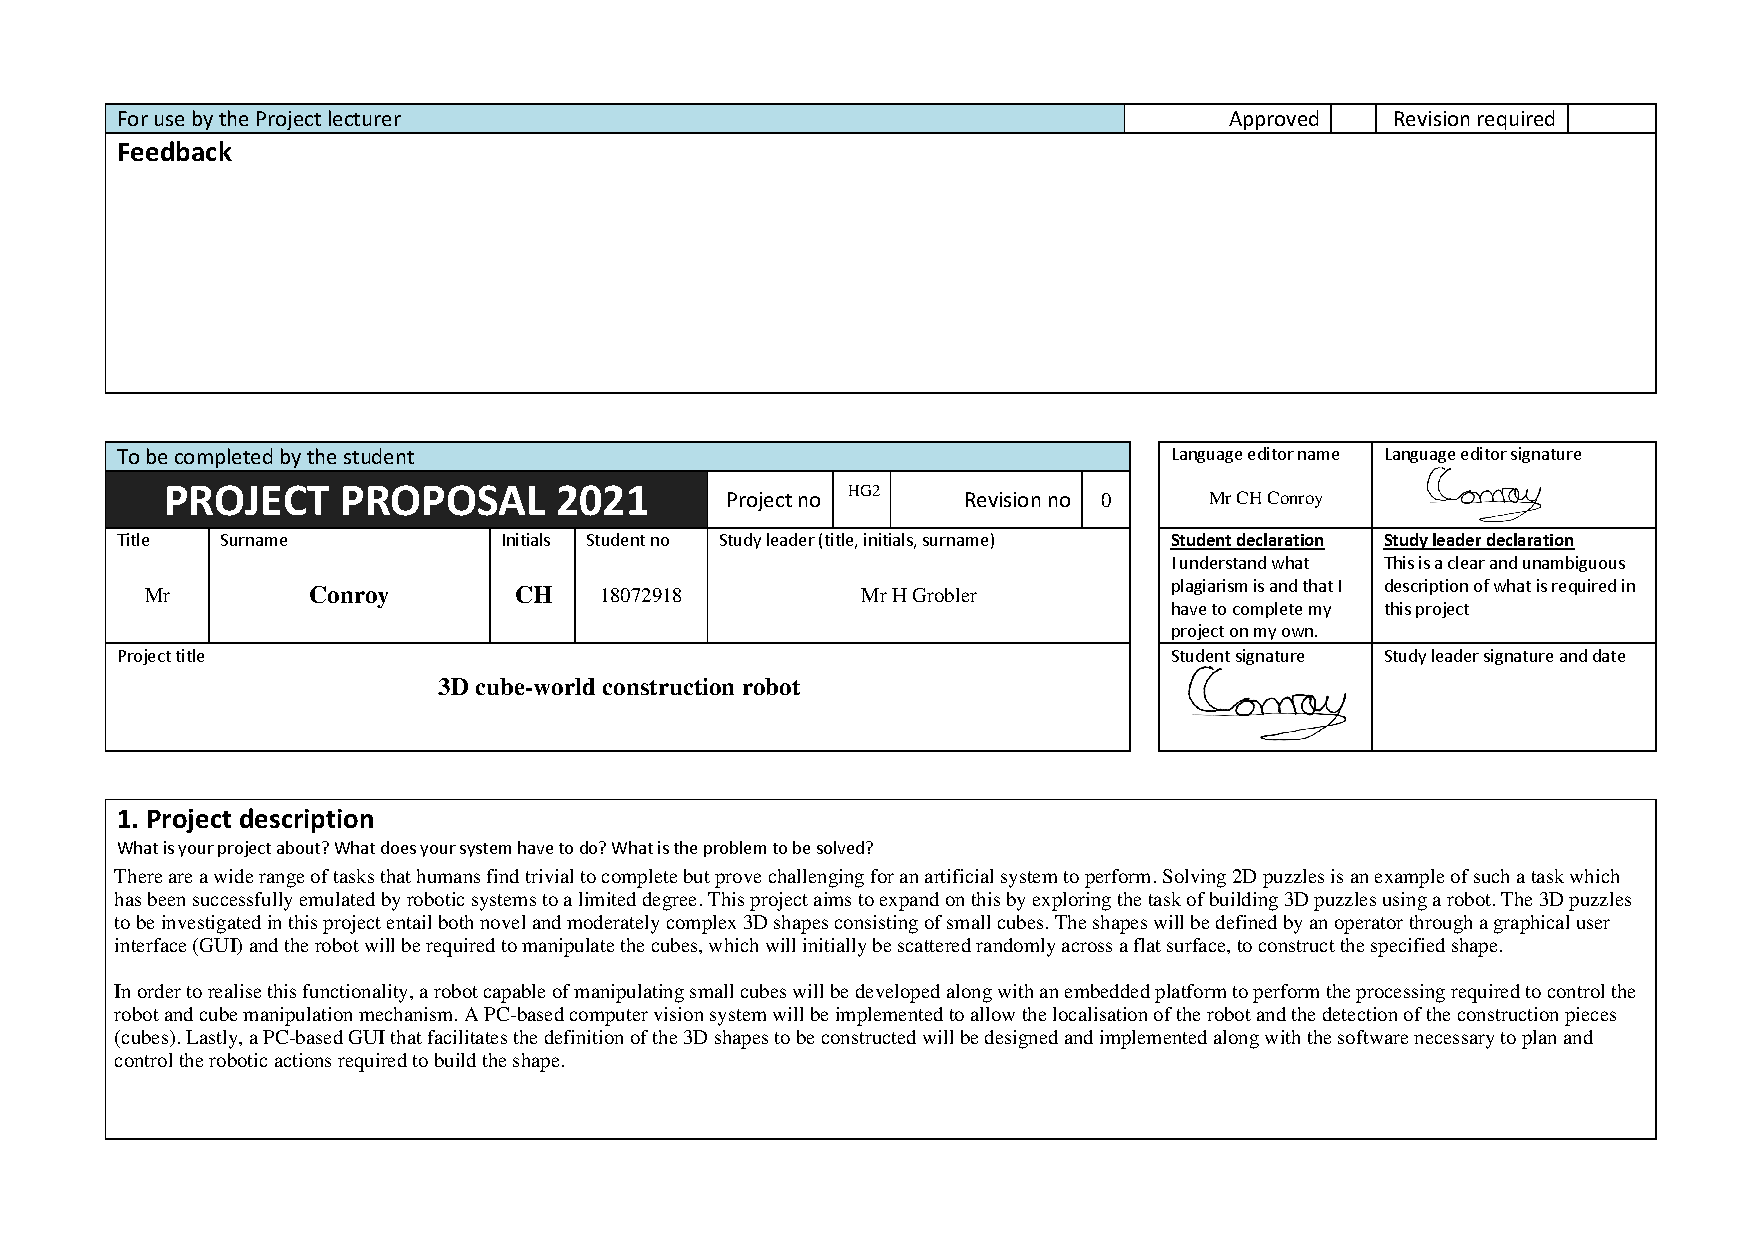
\includepdf[pages=-, landscape]{proposal.pdf}

%% --- PART 3 ------------------------------------------------------------

\eprsec{Part 3. Main Report}
\newpage

%% Reset the page number style and count.
\pagenumbering{arabic}
\setcounter{page}{1}

%% Import the main report content
%%
%%  Department of Electrical, Electronic and Computer Engineering.
%%  EPR400/2 Final Report - Section 1.
%%  Copyright (C) 2011-2021 University of Pretoria.
%%

\section{Literature study}

%%% ---[ BEGIN REMOVE ]---
%{\slshape
%Your literature study, described in the study guide, goes here.
%}
%%% ---[ END REMOVE ]---
%
%\subsection{Testing equation numbering}
%
%\begin{equation}
%  \Delta w_{i,j} = \alpha a_i \Delta[j]
%\end{equation}
%
%\nocite{Haykin:Communication_Systems}
%\nocite{*}

\subsection{Background}

% High-level task context

\subsubsection{Overview}

The use of artificial systems to emulate tasks that humans find straightforward to perform, such as solving 2D puzzles, has been a long-standing practice since components of the solution system are often relevant in industrial applications \cite{Burdea:Solving_Jigsaw_Puzzles_by_a_Robot}. This work focuses on a similar task that involves the construction of 3D shapes using small cubes. Such a task bears similarity to those tasks in the domain of pick and place robotics with the variation that object placement is dependent on the location of previously placed objects. Existing solutions in this domain typically consist of two primary components: a computer vision system to detect and localise the object of interest as well as a robot to alter the location and orientation of the object in 3D space \cite{Sharath:Gantry_Robot_Design}.

% Overall system literature

%- Compare in terms of robot used and in terms of object manipulated?
%
%Due to the wide range of variation possible in each of the subsystems, there exists a wide range of unique system - level approaches to solving related problems
%
%\cite{Lin:Character_Cube_Stacking_Robot} 
%- Robotic and computer vision research involving cube as the object of interest. In this case, the cubes contain markings that can be used to distinguish the cubes in images.
%- Charge-coupled device (CCD) camera was used
%- Used a previously produced robot. The robot used is a mobile robot with a size comparable to that of the cubes.
%- The orientation of the cube here about all axes of rotation is of concern while the only orientation of concern in this project is rotation about the vertical axis. Furthermore, the initial orientation of the cube could be arbitrary which is not the case in this project.
%- End effector mechanism similar to that of a gripper.
%- "Through the experiment we discovered that the biggest problem that affects the finding and recognizing of the letter  blocks  is  the  targeting  frame  becomes  unclear"

\subsubsection{Robotic System}

% Mechanical component of robotic system
% - Consider dividing into manipulator, end-effector and vacuum generation literature

A robot can be viewed as the combination of two core components, namely the robotic manipulator and the end-effector. The end-effector is the physical interface between the robot and the object of interest and is referred to as a robot gripper when its purpose is to grip the object to facilitate pose manipulation. The nature of the robot gripper depends on the physical characteristics of the object of interest and as such a wide variety of grippers have been developed. These include stiff finger grippers, flexible finger grippers, magnetic grippers and vacuum grippers which are best suited for objects with a flat surface \cite{Lundstrom:Industrial_Robot_Grippers}. The function of the robotic manipulator is to alter the position and orientation of the end-effector in 3D space. Robotic manipulators are categorised by the coordinate systems used to describe their movement mechanics which includes polar, cylindrical, articulate and Cartesian coordinates \cite{Miller:Robots_and_Robotics_Principles}. Cartesian robots have the benefit that accuracy of the robot is uniform throughout the robot's work envelope.

% Types of robots

% Robotic system motor control


% Embedded robot controller

\subsubsection{Object Detection}

% Object detection

The purpose of the computer vision system is to detect the object of interest and localise it using the input image data captured from the robot's workspace, such that the robot has sufficient information to interact with the object. It is important that a distinction is made between object detection and object recognition. Object detection refers to the process of locating instances of a given object within an image while object recognition refers to the identification and classification of an object. This work is concerned with the former as the object of interest is known to be a cube. There are a wide range of approaches to the object detection problem. These can be broadly classified as being part of either the traditional computer vision domain or the deep learning domain \cite{MathWorks:Object_Recognition}. In both cases, various techniques are used extract information from the image data in the form of features which are subsequently used to detect the objects of interest \cite{Kumar:Visual_Servoing}. 

The distinguishing factor between traditional and deep-learning domains lies in the method of feature extraction. Traditional approaches incorporate a manual feature extraction step before the data is processed further. Deep learning approaches, on the other hand, integrate this step as part of the underlying model, such as a convolutional neural network (CNN). In this sense, such models can be viewed as highly integrated structures which take images as input after minimal preprocessing and produce the object recognition information as output. An deep-learning approach has been developed to detect generic rectangular cuboid objects in everyday scenes captured from a single perspective \cite{Xiao:Localizing_3D_Cuboids}. However, the generic nature of this task requires a highly sophisticated approach to achieve reasonable success. 

% Classical image processing techniques
% - Low level feature detection
% - Contour detection
% -- Binary images vs gradient images etc
% - SIFT etc 

The best solutions to computer vision problems that arise from unconstrained environments and require a great degree of generality are almost always found in the deep learning domain. However, when the problem is sufficiently constrained, solutions based on traditional techniques often exhibit performance that is comparable or even superior to that of deep learning approaches. In such cases, traditional approaches are often preferable since, unlike deep learning approaches, they do not require a massive training data set or a large degree of computational power. In general, a feature can be considered to be a piece of information present within the image input data. Edges, corners, blobs and ridges are examples of common low-level features that are considered within the traditional computer vision domain. Feature detectors are used to locate these fragments of information in the image input data. The Canny edge detector \cite{Canny:Computational_Edge_Detection} and Harris corner detector \cite{ Harris:Corner_and_Edge_Detector} are examples of such methods which are popular for detecting edge and corner features respectively within an image.

The blurring of an image is a preprocessing step commonly employed with traditional approaches. This operation acts as a low-pass filter and filters out high-frequency noise which manifests itself as outlier pixel intensities. Improved performance of the feature detection stage is generally observed as a result. The conversion of an image to grey-scale is another common preprocessing step which reduces the complexity of subsequent operations when the color information of the image is insignificant. Thresholding is a useful method for obtaining shape-level feature information through image segmentation and is often applied following the preprocessing phase. The application of this technique to a grey-scale image results in a binary image which lends itself to further shape-level feature extraction. Since there are exposure inconsistencies that arise between images due to environmental light variability, it is usually prudent to incorporate an automatic threshold level determination mechanism when thresholding. In the ideal case, a grey image will exhibit a bimodal distribution of pixel intensities where the minima between the peaks corresponds to the ideal threshold value. However, such pixel intensity distributions are not necessarily guaranteed in most practical applications and, as a result, more robust automatic thresholding techniques have been developed, such as Otsu's method \cite{Otsu:Threshold_Selection_Method}. Existing automatic thresholding methods are usually classified as either histogram shape-based, clustering-based, entropy-based, object attribute-based, spatial or local methods \cite{Guruprasad:Overview_of_Thresholding_Methods}.

Contours are another useful shape-level feature that can be used in service of traditional approaches to object detection. The bounding outline that captures the shape of an object in an image is considered to be a contour. There are many different approaches to contour detection which, in general, can be categorised as either pixel-based, edge-based or region-based methodologies. Contours in images frequently correspond with discontinuities in grey-scale pixel intensity, particularly in the case of contours arising from luminance changes, which are detectable through the corresponding gradient magnitude information. A common approach to  extract this information is to make use of a local filter which is convolved with the image. This results in a gradient space where the greatest gradient magnitudes are indicative of potential contours. However, this method is unreliable as it usually produces discontinuous contours and, therefore, often requires supplementary high-level feature information \cite{Gong2018:Overview_of_Contour_Detection_Approaches}.

The contour detection problem is significantly simplified when the problem space is constrained to only binary images. In this case, gradient information is not required as with grey-scale images as pixel intensity discontinuities can be determined using only adjacent pixels. Furthermore, a binary image can be interpreted as consisting of a number of connected components where a connected component is defined as a set of pixels with identical intensity values which are interconnected through either 4-pixel or 8-pixel connectivity. Within this framework, the concept of a contour can be reduced to the sequence of pixels that define the boundary between adjacent but dissimilar connected components. The advantage of such contours is that they are guaranteed to be continuous, in contrast to the grey-scale image case. The border following algorithm is a longstanding approach to the detection of these binary image contours \cite{Suzuki:Binary_Image_Topological_Structural_Analysis}. An extension to this approach exists whereby a more advanced border labeling method is employed to facilitate the extraction of topological structure information. Such information includes the hierarchical relationship between borders as well the distinction between outer and hole borders. This approach has also been adapted such that only the top-level outer borders in the hierarchy are detected which offers improved computational performance for applications that only require such information \cite{Yokoi:Binary_Image_Topological_Properties_Analysis}.

Contour detection, in conjunction with contour template matching, has been successfully used in robotic object detection and grasping applications using a single monocular camera \cite{Wei:Robotic_Object_Recognition_With_Natural_Background}. There exist a number of other feature detectors which have applicability to cube detection. For objects with straight edges, the Hough transform is a useful image processing tool that can be used to capture these edges with parameterised straight lines in 2D space which is useful to determine the orientation of the object \cite{Aggarwal:Line_Detection_Hough_Transform}. A more advanced and robust approach to determining useful features within an image involves the use of a feature descriptor which is a vector of values that describes the local region about a given image point. A number of feature descriptor algorithms have been developed such as the scale-invariant feature transform (SIFT) \cite{Lowe:Distinctive_Image_Features_from_Scale_Invariant_Keypoints}, speeded-up robust features (SURF) \cite{Bay:SURF_Speeded_Up_Robust_Features}, features from accelerated segment test (FAST) \cite{Rosten:Machine_Learning_for_High_Speed_Corner_Detection}, binary robust independent elementary features (BRIEF) \cite{Calonder:BRIEF_Binary_Robust_Independent_Elementary_Features} and finally the oriented FAST and rotated BRIEF (ORB) \cite{Rublee:ORB_Alternative_to_SIFT_or_SURF} algorithms. These features can be used to detect instances of objects within the input image data through the process of template matching. This method has been successfully applied as part of the detection process for cubes marked with alphabetical and numerical characters \cite{Lin:Character_Cube_Stacking_Robot}.

% Object and robot localisation
% - Camera particulars
% -- Extrinsic and intrinsic matrices
% -- Camera calibration techniques
% --- Checkerboard calibration
% --- Distortion estmation and correction
% - Technqiues to determine extrinsic parameters
% -- Solve PnP approach
% - Techniques to identify known point points
% -- Fiducial markers

\subsubsection{Object Localisation}

The detection of an object within an image only forms the first stage in the robot's computer vision system. In order for the robot to interact with the object of interest in the physical world, the detected object needs to be localised such that its pose with respect to the robot's coordinate system is known. The object localisation methods available for robots when only red, green and blue (RGB) image input data is available can be categorised as either monocular vision or stereo vision approaches. With the monocular vision case, only a single RGB image is available as input at each time instance while in the stereo vision case, two or more RGB images are available \cite{Liu:6DOF_Object_Localization}. The primary drawback of monocular vision approaches is the loss of depth information that arises during the projection of the 3D world onto a single 2D image. An additional piece of information, such as the size or world plane of the object, is required in order to recover the depth information. Stereo vision approaches, on the other hand, are able to recover the depth data based on the disparity between images that arises due to difference in pose of the cameras used to capture the images \cite{Azad:Stereo-based_6D_Object_Localization}. However, stereo vision approaches require more hardware and greater computational resources than monocular vision approaches. An alternative approach is to make use of a device that captures red, green, blue and depth (RGBD) data directly, such as a time-of-flight (ToF) camera or integrated binocular stereo camera. 

In order to relate the object detection information derived the from camera input data to the world frame, the pose of the camera with respect to the world coordinate system needs to be determined. This information is represented by an extrinsic camera matrix which encompasses the rotation and translation parameters of the camera's pose with respect to the world frame. The extrinsic matrix can be used to map points in the world coordinate system to the 3D camera coordinate system. In order to map points from the 3D camera coordinate system to the 2D homogeneous coordinates in the image, an intrinsic camera matrix is used \cite{Szeliski:Computer_Vision_Algorithms_and_Applications}. Intrinsic parameters describe internal properties of the camera and are based on the pinhole camera model. These include the camera's inherent principal point offset, focal length and axis skew. The skew of the sensor axes occurs as a result of the optical axis not being exactly perpendicular to the sensor plane. However, for practical purposes this parameter is often discarded. The extrinsic matrix and intrinsic matrix can be multiplied to form the projection matrix which is used to project any point in the world frame to the image frame provided that the pinhole camera model is used and no lens distortion effects are present \cite{OpenCV:Camera_Calibration}.

The intrinsic and extrinsic camera parameters need to be determined in order to make use of the pinhole camera model in practical applications. Camera calibration is used to estimate the intrinsic characteristics of the camera while camera localisation is used to estimate the extrinsic parameters of the camera. A popular approach to camera calibration involves the use of a planar pattern with known dimensions of which multiple images are captured at various different poses \cite{Zhang:A_Flexible_Camera_Calibration_Technique}. Either the pose of the planar pattern or the camera may be altered between calibration images. The application of this algorithm to a given set of such images will produce an estimate of the intrinsic parameters of the camera as well as the radial distortion of the camera. Real-world cameras have lens-induced distortion effects that are not included as part of the pinhole camera model. Radial distortion is observed when the degree to which light rays bend when incident on the lens is not consistent with the distance from the optical centre of the lens. Tangential distortion is observed when a degree of misalignment exists between the image plane and lens. These distortion effects are described by the radial and tangential distortion coefficients respectively \cite{MathWorks:Camera_Calibration}.

In order to determine the extrinsic camera matrix, the rotation and translation of the camera with respect to the world coordinate system needs to be calculated. A popular approach to this problem involves the use of \textit{n} 3D to 2D point correspondences to calculate the camera pose for six degrees of freedom (DoF). A point correspondence refers to the situation where the 3D location of a given point in the world coordinate system as well as the corresponding 2D location in the homogeneous image frame are known. The most general formulation of this problem requires the computation of the camera's intrinsic parameters as well as the camera's extrinsic parameters. The Direct Linear Transform (DLT) algorithm is a well-known solution to this problem when at least six point correspondences are given \cite{OpenCV:Textured_Object_Pose_Estimation}. However, this approach suffers from a degree of inaccuracy due to the need to estimate the intrinsic parameters of the camera.

If the assumption is made that the camera is calibrated, such that the intrinsic parameters of the camera are known, the problem reduces to the Perspective-\textit{n}-Point (P\textit{n}P) problem which has been deeply explored in literature. As such, a number of iterative and non-iterative solutions to the P\textit{n}P problem have been developed. The efficient P\textit{n}P (EP\textit{n}P) algorithm is a popular non-iterative approach for the case when four or more point correspondences are given. Although four point correspondences is sufficient for EP\textit{n}P to find a solution, a greater number is preferred to provide a degree of redundancy and reduce the solution's sensitivity to noise. It is also noted that the algorithm is capable of solving for the case where the points used for the point correspondences have a planar arrangement in the world coordinate system \cite{Lepetit:EPnP}.

Within the context of the P\textit{n}P problem, the first step to solve for the camera's extrinsic parameters requires the creation of a set of point correspondences. The use of fiducial markers is a popular approach to this task, notably in the augmented reality domain. In general, a marker is an object that is placed as known point of reference in the scene that is processed by the computer vision system. A fiducial marker system consists of three core components, namely the markers, a fiducial detector and an encoding scheme. The fiducial detector typically makes use of traditional computer vision techniques and are therefore usually characterised by simple designs that are distinct within the scene \cite{Zhang:DeepTag_General_Framework_for_Fiducial_Marker_Design}. Morphological operations often form part of the traditional methods applied during the marker detection stage  \cite{Kostak:Designing_a_Simple_Fiducial_Marker}. 

The design of the marker ensures it is rotationally asymmetric while encoding a piece of information such as the fiducial identifier. Some existing fiducial families, such as ARToolkitPlus \cite{Wagner:ARToolKitPlus} and AprilTag \cite{Olson:AprilTag}, make use of black and white square grids to encode binary data where each cell represents a binary digit. In order to extract information from the markers, perspective distortion needs to be eliminated. In the case of square markers, the corners of each marker candidate are used to compute a homography that is used to remove this distortion \cite{Hirzer:Marker_Detection_for_Augmented_Reality_Applications}. Finally, a unique marker with a known location in the world coordinate system can be used to create a point correspondence through the combination of this information with its detected location in the image coordinate frame. The use of multiple markers facilitates the creation of the requisite point correspondence set.

% Computer graphics
% - Existing APIs, frameworks
% - OpenGL

\subsection{Applicability to Project}

% >> Reflection
% Brief summary of how you applied the above background (one to two pages)
% Summarises what has been learnt in the literature study and describes how you applied what you learnt from literature (and perhaps expanded what has been reported on before in the literature)

There exists a substantial amount of literature exploring the field of artificial systems and their application in various problem domains. Problems addressed by artificial system solutions in the domain of pick and place robotics are generally the most closely related to the 3D shape construction task explored in this project. It was noted that, at a system level, solutions in this domain typically consist of a computer vision system used in conjunction with a robot. This information, in addition to the implementation details of these systems, was used as a starting point to guide the system-level design in this project.

In terms of the robotic system, the general approach to the mechanical design of a robot can be partitioned into the design of two distinct components, namely the robotic manipulator and the end-effector. The literature highlights a wide variety of approaches to the design of both these mechanical facets. In both cases, the selection of a particular approach depends substantially on the the nature of the problem space. Fortunately, there is an expansive body of knowledge in terms of the strengths and weaknesses for each of the approaches for both the end-effector and the robotic manipulator with respect to a number of problem domains. As such, the literature was used as the basis for the mechanical design approach selected decisions made in this project. In addition, the machine design procedure frequently appears as a core component of the mechanical design process in similar projects. Therefore, this procedure was also incorporated into the robot design process utilised in this project.

% Discuss object detection
The detection and localisation of the constituent construction cubes by the computer vision system is an essential component of this project that is required to facilitate interaction of the robot with dropped cubes. Fortunately, there exists a vast range of literature in the computer vision field that has direct applicability to this problem. For the cube detection component of this problem, there are two broad potential solution domains, namely the deep-learning and traditional computer vision domains. Solutions in the deep-learning domains are typically best applied to problems that require a significant degree of generality while traditional solutions are best suited to constrained problems. Traditional detection solutions are based on the manual extraction of selected features from the object of interest which are subsequently used to identify instances of the object in arbitrary images. A number of methods that are useful for extracting such features were identified in this literature study and many of these were trialed in application to the cube detection problem in this project. The methods that exhibited the greatest degree of accuracy and robustness when applied were included as part of the final computer vision system implementation.

% Discuss object localisation
Once a cube has been detected within the input image data, the location and orientation of the cube needs to be determined with respect to the robot in the physical world. This relates to the problem of object localisation which has been explored extensively in literature, particularly in the augmented reality and robotic system domains. The exact nature of the solution depends on whether a monocular or stereo vision approach is used. In general, existing solutions build on the mathematical foundation provided by the pinhole camera model. This model formed the basis of describing the relationship between the robot and camera coordinate system's in this project. The intrinsic and extrinsic camera parameters outlined within this model are sufficient to facilitate the projection of points between the coordinate systems. This was taken advantage of to determine the location of cube points with respect to the robot from the corresponding points in the input image data.

In order to make practical use of the above object localisation approach, the intrinsic and extrinsic camera parameters need to be determined. The camera calibration techniques identified in literature offer an avenue to determine the intrinsic matrix of the camera and these were subsequently applied to calibrate the camera used in this project. Similarly, solutions to the P\textit{n}P problem provide a means to determine the extrinsic camera parameters and, as such, one of the identified solutions from the literature was utilised to determine the camera extrinsics in this project. Furthermore, any solution to the P\textit{n}P problem requires a set of point correspondences between the world frame and the image frame. Existing approaches make use of fiducial markers to obtain these correspondences and the same approach was applied in this project. Furthermore, a number of the papers included as part of the this literature study detail a wide variety of fiducial marker design considerations. These was used to inform the design of the fiducial markers used in this project.

% Discuss differences and conclude
Overall, there have been a number of research projects into artificial systems, consisting of a computer vision system used in conjunction with a robot to perform tasks such as 2D puzzle building or generic pick and place operations. However, the specific task of constructing moderately complex 3D shapes using small cubes does not appear to have been explored. A similar project involved the use of larger cubes marked with identification artifacts to assist in the detection of the cubes \cite{Lin:Character_Cube_Stacking_Robot}. In contrast, the cubes used in this project exhibit a plain appearance and a greater degree of reflectivity due to their metallic nature. In general, the majority of the approaches only focus on the development of a particular sub-component of the robotic and computer vision system while the bulk of the system comprises of an off-the-shelf implementation adapted to support the task in question. This work aims to develop a robot in conjunction with a computer vision system with all components tailored to fulfil the 3D shape construction task.

\newpage

%% End of File.

%%
%%  Department of Electrical, Electronic and Computer Engineering.
%%  EPR400/2 Final Report - Section 2.
%%  Copyright (C) 2011-2021 University of Pretoria.
%%

\section{Approach}

\subsection{Problem Space}

The nature of the selected approach to the cube construction task explored in this project is completely dependent on the characteristics of the problem space. The problem space was broadly defined as part of the project proposal. However, further details regarding the cube component of the problem space are required in order to justify the chosen approach. A number of general materials were considered to form the construction cubes including hard plastic, wood, aluminium and steel. Hard plastic cubes have the advantage that they are widely available off-the-shelf while wood offers ease in cube manufacturing. However, the low density of these materials means the cubes are more likely to shift in the shape structure when exposed to vibrations. Therefore, aluminium cubes were chosen due to their greater density. Aluminium was selected over steel due to its superior machinability and inability to rust.

\subsection{Robotic Subsystem}

The robotic subsystem (FU3) was identified as one of the major components of the solution system from a functional perspective in the project proposal. The high-level purpose of FU3 is to facilitate the manipulation of the construction cube's pose in 3D space. The robotic end-effector (FU3.5) acts as the robot's physical interface with the cube. Grippers are commonly used for the end-effector components. However, there exist planar arrangements of adjacent cubes that prevent access to at least one opposite face pair of the target cube which is required by the gripper to exert a grip. Therefore, a vacuum-based suction cup end-effector mechanism was selected as it only requires access to the top face of the target cube to exert a grip. Furthermore, the non-porous and smooth nature of the aluminum cubes render the cube amenable to this mechanism.

 There are a wide range of approaches to the robotic manipulator component (FU3.4) which is required to manipulate the end-effector pose in 3D space. These include the articulated robot, selective compliance articulated robot arm (SCARA), delta robot and the Cartesian robot. The articulated robot offers the greatest flexibility in the range of poses the robot can attain while the delta robot offers excellent movement speed. However, these kinematics of these robots are complex and minor imperfections in their implementation creates inaccuracy. Furthermore the precision of these robots, in addition to SCARA robots, varies throughout the workspace. Cartesian robots, on the other hand, exhibit consistently high precision throughout the workspace and are suited to Cartesian-based problems. A Cartesian gantry robot was selected as the robotic manipulator approach for these reasons. The robot was designed outwards from its interface with the cube in an iterative fashion  using computer-aided design (CAD) software and a mathematical base in dynamics.
 
 The robotic controller (FU3.2) was designed as an embedded platform to provide an interface to control the robotic manipulator and end-effector. This component was first designed and prototyped using a breadboard before a more robust PCB implementation was developed. The embedded software for this controller was prototyped using the STM32 hardware abstraction layer (HAL) library before being converted to first principles. The power supply (FU3.6) was taken off-the-shelf as well as the motor drivers (FU3.3). Finally, the communication unit (FU3.1) was based on the universal asynchronous receiver-transmitter (UART) and realised as a custom communication protocol used in conjunction with an off-the-shelf CH340 serial converter integrated circuit (IC).

\subsection{PC-Based Software Component}

The PC-based software component (FU2) was developed as a graphical user interface (GUI) application using C++ and the QT framework. C++ was selected due to the suitability of its performance to the computationally intensive nature of the image processing required in this project. QT was selected due to its maturity and support for OpenGL integration. FU2 was explored and developed in a bottom up approach. This means that the shape definition component (FU2.1) and cube detection and localisation component (FU2.2) were designed and developed first followed by the system controller (FU2.3), construction planner (FU2.4) and robotic motion planner (FU2.5) which all depend on FU2.1 and FU2.2. OpenGL was selected as the low-level graphics API to implement the 3D shape model render required by the shape definition component. This component was originally developed externally to the QT ecosystem to verify its functionality before being integrated adapted for integration with the QT OpenGL interface.

A number of object detection approaches were investigated for cube detection in FU2.2. However, a binary thresholding approach based on the reflection intensity of light from the top cube faces was found to be the most robust and used in conjunction with contour detection. A pin-hole camera model based approach was used to map points between the image and world frames for the purpose of cube localisation in FU2.2. These components were initially developed using the OpenCV library before being progressively replaced with first principle implementations.

Finally the system controller was developed simultaneously with the construction planner and the robotic motion planner in a tightly integrated manner. As the system controller acts as the central point that where the information pathways from the shape definition unit, cube detection and localisation unit and the robotic subsystem intersect, the system controller was developed as the top-level component in the PC-based software that integrates the other software components. As a result, the primary high-level software design work took place as part of the development of this component.

The approach reasoning and considerations discussed here correspond directly to the structure of the system design presented in Section \ref{sec:Design and Implementation}. Specifically the design of the robotic subsystem is first presented in two parts, namely the mechanical design in Section \ref{sec:Mechancial Robotic Component} followed by the embedded controller design in Section \ref{sec:Embedded Robot Controller}. The design of the PC-based software is then presented in three parts. The first two parts are the shape definition component in \ref{sec:Shape Definition Interface} and the computer vision component in Section \ref{sec:Computer Vision System} on which the system controller depends. Finally the system controller and the use of this component as the basis for system integration is presented in Section \ref{sec:System Controller}.


\newpage

%% End of File.


%%
%%  Department of Electrical, Electronic and Computer Engineering.
%%  EPR400/2 Final Report - Section 3.
%%  Copyright (C) 2011-2021 University of Pretoria.
%%

\section{Design and implementation} \label{sec:Design and Implementation}

% Note on notation and conventions
% Contour detection
% - 

\subsection{Design summary}

This section presents a summary of the project design tasks as well as the implementation of these tasks (see Tables \ref{tab:design_summary_p1}-\ref{tab:design_summary_p2}).

\begin{table}[H]
	\renewcommand{\arraystretch}{1.3}
	\centering
	\begin{tabular}{|>{\raggedright}m{5cm}|>{\raggedright}m{5cm}|>{\raggedright\arraybackslash}m{4cm}|}
		\hline
		\textbf{Deliverable or task} & \textbf{Implementation} & \textbf{Completion of deliverable or task, and section in the report} \\
		\hline
		Mechanical design and construction of robotic manipulator & The mechanical design of the robot manipulator was completed from first principles using the Fusion 360 CAD software. This was constructed by the student both using 3D printing and metal machining technologies. & \\
		\hline
		Mechanical design and construction of robotic end-effector mechanism & The mechanical design of the robotic end-effector mechanism was completed from first principles using the Fusion 360 CAD software. This was constructed by the student using 3D printing technologies. & \\
		\hline
		Design of embedded robot controller circuit & The design was completed from first principles and a prototype was implemented on a breadboard. & \\
		\hline
		Design of printed circuit board (PCB) for embedded robot controller & The PCB design was completed using the KiCAD software package from first principles. & \\
		\hline
		Development of firmware for embedded robot controller & Firmware was developed from first principles using C. & \\
		\hline
		Design of communication protocol for communication between the embedded robot controller and the PC-based software & The communication protocol design was completed from first principles and implemented between the embedded robot controller and PC. & \\
		\hline
		Design and implementation of shape definition GUI based on a low-level graphics application programming interface (API) & The shape definition GUI was designed and implemented from first principles using the OpenGL graphics API. & \\
		\hline
	\end{tabular}
	\caption{\label{tab:design_summary_p1}Design summary.}
\end{table}

\begin{table}[H]
	\renewcommand{\arraystretch}{1.3}
	\centering
	\begin{tabular}{|>{\raggedright}m{5cm}|>{\raggedright}m{4cm}|>{\raggedright\arraybackslash}m{4cm}|}
		\hline
		Development of computer vision cube detection algorithm & The computer vision cube detection algorithm was developed mostly from first principles using C++. A few basic image image processing functions were used from OpenCV. & \\
		\hline
		Development of computer vision cube localisation algorithm & The computer vision cube detection algorithm was developed mostly from first principles using C++. A few basic image image processing functions and camera calibration functions were used from OpenCV. & \\
		\hline
		Development of construction planner software component & The construction planner software component was developed from first principles. & \\
		\hline
		Development of robotic motion planner software component & The robotic motion planner software component was developed from first principles & \\
		\hline
		Development of system control software that integrates the shape definition, computer vision, construction planner and robotic motion planner software components & The system control software was developed from first principles using the QT C++ framework. & \\
		\hline
	\end{tabular}
	\caption{\label{tab:design_summary_p2}Design summary continued.}
\end{table}

\subsection{Mechanical Robotic Component} \label{sec:Mechancial Robotic Component}

\subsubsection{End-Effector Mechanism}

For the purposes of this project, the end-effector subsystem refers to the components responsible for enabling the direct manipulation of the cube. These components include the vacuum pad, tubing and vacuum generation system. The end-effector subsystem is attached to the gantry robot by means of an end-effector mechanism. In order to design this component, the machine design procedure was followed. The first step of this procedure involves understanding the requirements of the machine. The end-effector mechanism requirements are listed below. The end-effector mechanism should:

\begin{compactitem}
	\item Attach the end-effector to the gantry robot.
	\item Maintain the suction-pad component in a vertical orientation.
	\item Allow limited linear buffered motion of the vertical suction-pad component along the z-axis w.r.t the gantry robot.
	\item The linear buffer should facilitate at least a 5mm range of linear motion.
	\item The purpose of the linear buffer is to allow the robot to target a z-axis position slightly below the intended z-axis position to ensure the cube is definitely touching the placement surface so the cube is not released in mid-air.
	\item Allow the vertical suction-pad components to rotate about the z-axis.
	\item Allow the connection of a drive mechanism to drive the rotation about the z-axis.
	\item Allow the vacuum tubing to be routed to the gantry robot.
\end{compactitem}

The initial design investigated for the end-effector mechanism was centred around the requirement of a 5mm linear displacement buffer. A buffer can be implemented as a linear rod with guide holes as well as a ridge on the rod that allows a spring to be placed between the ridge and one of the guide holes. This provides a linear buffering action along the axis to which the rod is aligned. The design idea with respect to the end-effector mechanism is to mount the vacuum pad on the end of the rod opposite to the spring and position the rod in a vertical orientation with the vacuum pad at the bottom where it can access cubes on the plane below it. When the vacuum pad is not in contact with anything, the spring and the force of gravity push the vacuum pad into its lowest position. When a force is applied vertically upwards against the vacuum pad, as is the case when the vacuum pad is pressed against a cube, the spring will compress if the force is greater than the gravitational force on the moving rod as well as the spring force at that length.

An issue with this simple design is that the vacuum tube needs to be routed to the vacuum pad as well as the fact that the vacuum pad needs to be rotatable by an external motor. The tubing routing issue is solved by making the rod hollow and routing the tube through the rod and out top of the rod. Furthermore, it is noted that the system only needs to be able to rotate a minimum of 90 degrees to be able to realise any orientation of a cube in terms of rotation about the z-axis. The rubber tubing is comfortably able to absorb this degree of torsion and therefore, no additional mechanisms are required to route the tube.

The second design consideration is how the rod will be rotated to rotate the vacuum pad given that the rod has linear motion of 5mm. The design solution to this investigated in the proof of concept design is the use of a gear attached to the rod which can be driven by a motor gear. The use of gears with their axes aligned with the rod axis allows the linear motion to be absorbed by the linear freedom of movement between the gear teeth. In order to absorb this motion, the height of the gear attached to the rod needs to be at least 5mm greater than the height of the motor gear is the maximum overlap is to be always maintained assuming the position of the motor is fixed with respect to the component supporting the rod. An alternative design that could be explored in the future, is fixing the linear position of the motor with respect to the spring to reduce the gear height and using the weight of the motor to act in a similar manner to the spring force.

%Rotary Motor Selection Considerations

The rod designed to facilitate the rotation and linear buffer motion of the vacuum pad was further developed. Intuitively, the rod requires a relatively low amount of torque to initiate and maintain rotary motion. Therefore, the smallest class of NEMA stepper motors, namely NEMA 8 motors, were considered as a guide for the motor footprint in the mechanical design. A preliminary decision to use a stepper motor over a servo was made based on the fact that rotary stability is essential once the vacuum pad has reached its required orientation. Servos may pulsate at standstill which is undesirable as the gripped cube may displace adjacent cubes. Furthermore, the rotation speed required is low and stepper motors exhibit the best torque characteristics at low speed. Lastly, in full step mode, NEMA 8 stepper motors typically exhibit a full step resolution of $1.8 ^\circ / \text{step}$ which falls within the rotary accuracy specifications of $5 ^\circ$.

%Transmission Gear Design

The width and breadth of the front face of the NEMA 8 stepper motor is 20 mm and 20 mm. The diameter of the designed rotary rod is 13 mm. In order to facilitate a sufficient space between the motor and the rotary rod for spring and rotary rod gear, the centres of rotation of the rotary rod and the NEMA 8 stepper motor were placed 20 mm apart. Since the step accuracy of the motor is sufficient, no gearing ratio is required. Therefore, the most space efficient manner of connecting these two rotary centres is with two gears with a pitch diameter of 20mm each. Since this is not a specialised application of these gears, relatively standard parameters were selected for their design. The gear parameters as designed in Fusion 360 and used for both gears are as follows:

\begin{compactitem}
	\item Pressure Angle = $20 ^\circ$
	\item Module = 1
	\item Number of Teeth = 20
	\item Backlash = 0.3 mm
	\item Root Fillet Radius = 0.3 mm
	\item Pitch Diameter = 20 mm
\end{compactitem}

A relatively large backlash of 0.3 mm was selected due to the high tolerance required by 3D printed parts. A pressure angle of $20 ^\circ$ and $25 ^\circ$ are the most commonly used angles in gear design. A smaller pressure angle has weaker teeth but runs quieter. Due to the low torque nature of this gear application, a $20 ^\circ$ pressure angle was selected to take advantage of the qualitative low noise benefit.

%Torque Calculations

The point of entry for calculating the various mass elements that need to be translated and rotated is the aluminium cube that needs to be manipulated. The density of aluminum is $2.7 g/cm^3$. Since the cube has a maximum side length of $1.3 cm$, the cube has a maximum mass of $5.94 g$. Using the updated design of the end-effector rod, the 3D model was converted to a triangle mesh and exported to the 3D printing slicer Cura. Using PLA 1.75mm filament, Cura estimated the weight of the part to be 7g when printed at 50\% infill. The following is a summary of the masses of the components that comprise the rotating mass in the end-effector as well as the mass of the cube gripped by the end-effector:

\begin{compactitem}
	\item Aluminium cube mass = 5.94 g
	\item 3D printed rotary rod at 50\% infill = 7 g
	\item ZPT08UN-B5 vacuum pad = 6 g
	\item M-5AU-6 barbed connector = 1.8 g
	\item Total mass = 20.74 g
\end{compactitem}

The system does not have any explicit angular velocity and angular acceleration specifications that it is required to meet from the project proposal. Therefore, it is decided that on a qualitative basis that the end-effector should be capable of completing a single rotation once every 4 seconds when at maximum velocity. Similarly, it is also decided that the end-effector should be capable of reaching this speed in 0.5 seconds from standstill. The angular velocity is computed as shown below in Equation \ref{eqn:angular-velocity}.

\begin{align}
	\omega&=\frac{\Delta \theta}{\Delta t}
	\label{eqn:angular-velocity} \\
	\omega&=\frac{2\pi}{4}=\frac{\pi}{2} \text{ rad/s}
\end{align}

The maximum angular acceleration the motor should be capable of driving is as calculated in Equation \ref{eqn:angular-acceleration} below assuming that the system accelerates linearly to the maximum velocity from standstill.

\begin{align}
	\alpha&=\frac{\Delta \omega}{\Delta t} 
	\label{eqn:angular-acceleration} \\
	\alpha&=\frac{\pi / 2 - 0}{0.5 - 0}=\frac{\pi}{4} \text{ rad/s}^2
\end{align}

In order to calculate the torque required to rotate the end-effector component, the moment of inertia $I_O$ about the centre of rotation $O$ of the component needs to be computed. The component is modeled as a cylinder with a radius of 10 mm and all of its mass located in its outer shell only. This is the cylindrical configuration that has the greatest moment of inertia and therefore requires the greatest torque to rotate. This guarantees that a motor capable of rotating this is capable of rotating the actual component. The moment of inertia for the cylindrical model is calculated as shown in Equation \ref{eqn:moment-of-inertia} below

\begin{align}
	I_O&=mr^2
	\label{eqn:moment-of-inertia} \\
	I_O&=(20.74 \times 10^{-3})(10 \times 10^{-3})^2=2.074 \times 10^{-6} \: kg\cdot m^2
\end{align}

where $m$ is the mass of the cylinder and $r$ is the radius of the outer shell of the cylinder. In order to relate the kinematic motion of the rotary end-effector component to the external forces applied to it, the moment equation for rotation about a fixed axis $O$ shown in Equation \ref{eqn:moment-equation} below can be used

\begin{align}
	\sum M_{Oi} = I_O \alpha
	\label{eqn:moment-equation} \\
	\sum F_i r_i = I_O \alpha
\end{align}

where $M_{Oi}$ is the moment that results from the application of force $F_i$ at the $i^{th}$ point at perpendicular distance $r_i$ from the axis of rotation $O$. Two external forces to the rotary end-effector component are considered, namely the force of static friction $F_{fs}$ and the force $F_A$ applied to the component gear by the gear on the motor's drive shaft. Only static friction is considered as it is generally greater than kinetic friction and therefore more challenging to overcome. The coefficient of static friction for plastic on plastic used in these calculations is $\mu _s = 0.4$. Furthermore, it is assumed that the friction only acts along the outer edge of the cylinder model since this is requires the most torque to overcome. $F_{fs}$ is computed as shown in equation Equation \ref{eqn:static-friction} below

\begin{align}
	F_{fs}=\mu _s \times F_N
	\label{eqn:static-friction}
\end{align}

where $F_N$ is the normal force from the weight of the end-effector component on the bottom support. Using Equation \ref{eqn:moment-equation}, the force required to accelerate the end-effector component from standstill at the required rate can be calculated as shown in Equation \ref{eqn:Fa-required}

\begin{align}
	&F_A r_A - F_{fs} r_{fs} = I_O \alpha
	\label{eqn:Fa-required} \\
	&F_A (10 \times 10^{-3}) - [(0.4)(20.74 \times 10^{-3})(9.81)] (10 \times 10^{-3}) = (2.074 \times 10^{-6})\left(\frac{\pi}{4}\right) \\
	&F_A = 81.52 \times 10^{-3} \, N
\end{align}

where $r_A$ and $r_{fs}$ are the distances between the point of force application and the centre of rotation O and for the forces $F_A$ and $F_{fs}$ respectively. Since the gear on the motor shaft is to be 3D printed, its mass is taken to be negligible. Since the pitch circle radius $r_m$ of the motor gear is 10 mm, the torque $\tau$ required to be generated by the motor in order to exert $F_A$ on the end-effector rotor is calculated as shown in Equation \ref{eqn:end-effector-motor-torque} below.

\begin{align}
	& \tau = F_A \times r_m
	\label{eqn:end-effector-motor-torque} \\
	& \tau = (81.55 \times 10^{-3}) \times (10 \times 10^{-3}) \\
	& \tau = 815.2 \times 10^{-6} \: N \cdot m
\end{align}

Using an engineering safety factor of 2 to account for inaccuracies in modeling the end-effector rotor and to ensure there is at least a 50\% torque margin for the motor, a minimum required motor holding torque of $1.63 \times 10^{-3} \; N \cdot m$ or $16.63 \; g \cdot cm$. Using the Wantai Motor product line as a reference, the smallest available stepper motor is the 20BYGH202 model which has a holding torque of $\tau_H=140 \; g \cdot cm$, detent torque of $\tau_D=20 \; g \cdot cm$ and a mass of $50 \; g$. The detent torque of the motor refers to the amount of torque generated by the motor when the windings of the motor are not energized. The holding torque, on the other hand, is the amount of torque required to rotate the motor one step when the rotor is stationary but the windings are energized. The running torque $\tau_R$ of the motor is limited by the motor's current rating and at low speeds is equal can be calculated using Equation \ref{eqn:running-torque} below.

\begin{align}
	& \tau_R = \tau_H - 2\tau_D
	\label{eqn:running-torque}
\end{align}

The running torque of the 20BYGH202 model is calculated as $\tau_R=100 \; g \cdot cm$ which comfortably meets the torque requirement of $16.63 \; g \cdot cm$. The excess torque can be used to implement greater acceleration or micro-stepping functionality. In the interest of keeping costs down for the project, the ISG component bank was considered when sourcing the motor. The smallest NEMA 8 motor contained in the bank was the 20BYGH406 which has a holding torque of $\tau_H=260 \; g \cdot cm$, detent torque of $\tau_D=50 \; g \cdot cm$ and a mass of $80 \; g$ which yields a running torque of $\tau_R=160 \; g \cdot cm$ which also comfortably meets the torque requirement. The additional $30\;g$ of mass was considered acceptable for the project and, therefore, the 20BYGH406 model was selected as the end-effector motor.

Vacuum Actuator

The measured dimensions of the syringe tube are as follows:

\begin{compactitem}
	\item Outer diameter = 20.80 mm
	\item Inner diameter = 18.60 mm
	\item Length (excluding nozzle) = 97.00 mm
	\item Length (including nozzle) = 108.00 mm
	\item Nozzle length = 11.00 mm
	\item Nozzle base ridge diameter = 6.24 mm
	\item Nozzle base ridge height = 2.04 mm
	\item Nozzle base diameter = 4.50 mm
	\item Nozzle top outer diameter = 4.00 mm
	\item Nozzle top inner diameter = 2.14 mm
	\item Shortest distance from nozzle base to main outer tube outer diameter = 1.14 mm
	\item Flange diameter = 23.55 mm
	\item Flange overall length = 37.04 mm
	\item Flange thickness = 1.60 mm
	\item Flange edge length = 12.80 mm
\end{compactitem}

The dimensions of the syringe plunger are as follows:

\begin{compactitem}
	\item Flange diameter = 21.70 mm
	\item Flange thickness = 1.60 mm
	\item Flat strut width (wide section) = 18.00 mm
	\item Flat strut width (narrow section) = 13.24 mm
	\item Strut width transition offset from flange (initial) = 13.30 mm
	\item Strut width transition offset from flange (final) = 19.90 mm
	\item Length = 111.00 mm
	\item Rubber height = 9.609 mm 
	\item Flat strut thickness = 1.20 mm
	\item Rubber end piece height = 9.00 mm
\end{compactitem}

The syringe has a maximum range of linear travel of 78 mm. The servo has a maximum range of rotational motion of $180^{\circ}$. Therefore, in order to achieve the full range of linear motion for the syringe, the mechanism connecting the servo to the syringe needs to translate the servo's $180^{\circ}$ of rotational motion into 78 mm of linear motion. A rack and pinion system is a mechanism that is commonly used for converting translational motion into rotational motion. Therefore, half of the circumference of the pitch diameter circle of the gear needs to be equal to the length of linear travel for these specifications to be achieved. A gear with a pitch diameter of 49.66 mm satisfies this requirement. Therefore, it was selected to use a gear with a pitch diameter of 50 mm. The mechanical connection mechanism to connect the syringe to the servo motor is shown as a 3D model in Figure \ref{fig:vacuum-actuator-model} as well as the physical realisation in Figure \ref{fig:vacuum-actuator} below.

\begin{figure}[H]
	\centering
	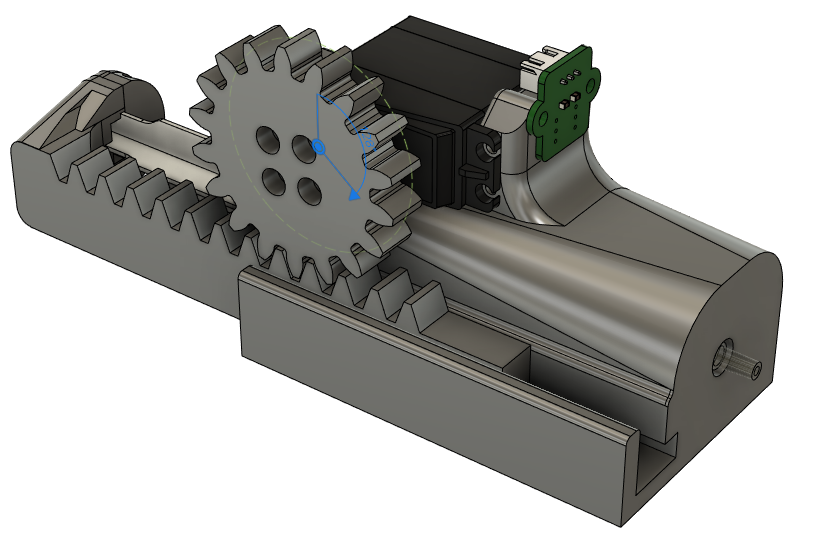
\includegraphics[width=0.6\linewidth]{figures/vacuum-actuator-model.PNG}
	\caption{3D model of vacuum actuator designed in Fusion 360.}
	\label{fig:vacuum-actuator-model}
\end{figure}

\begin{figure}[H]
	\centering
	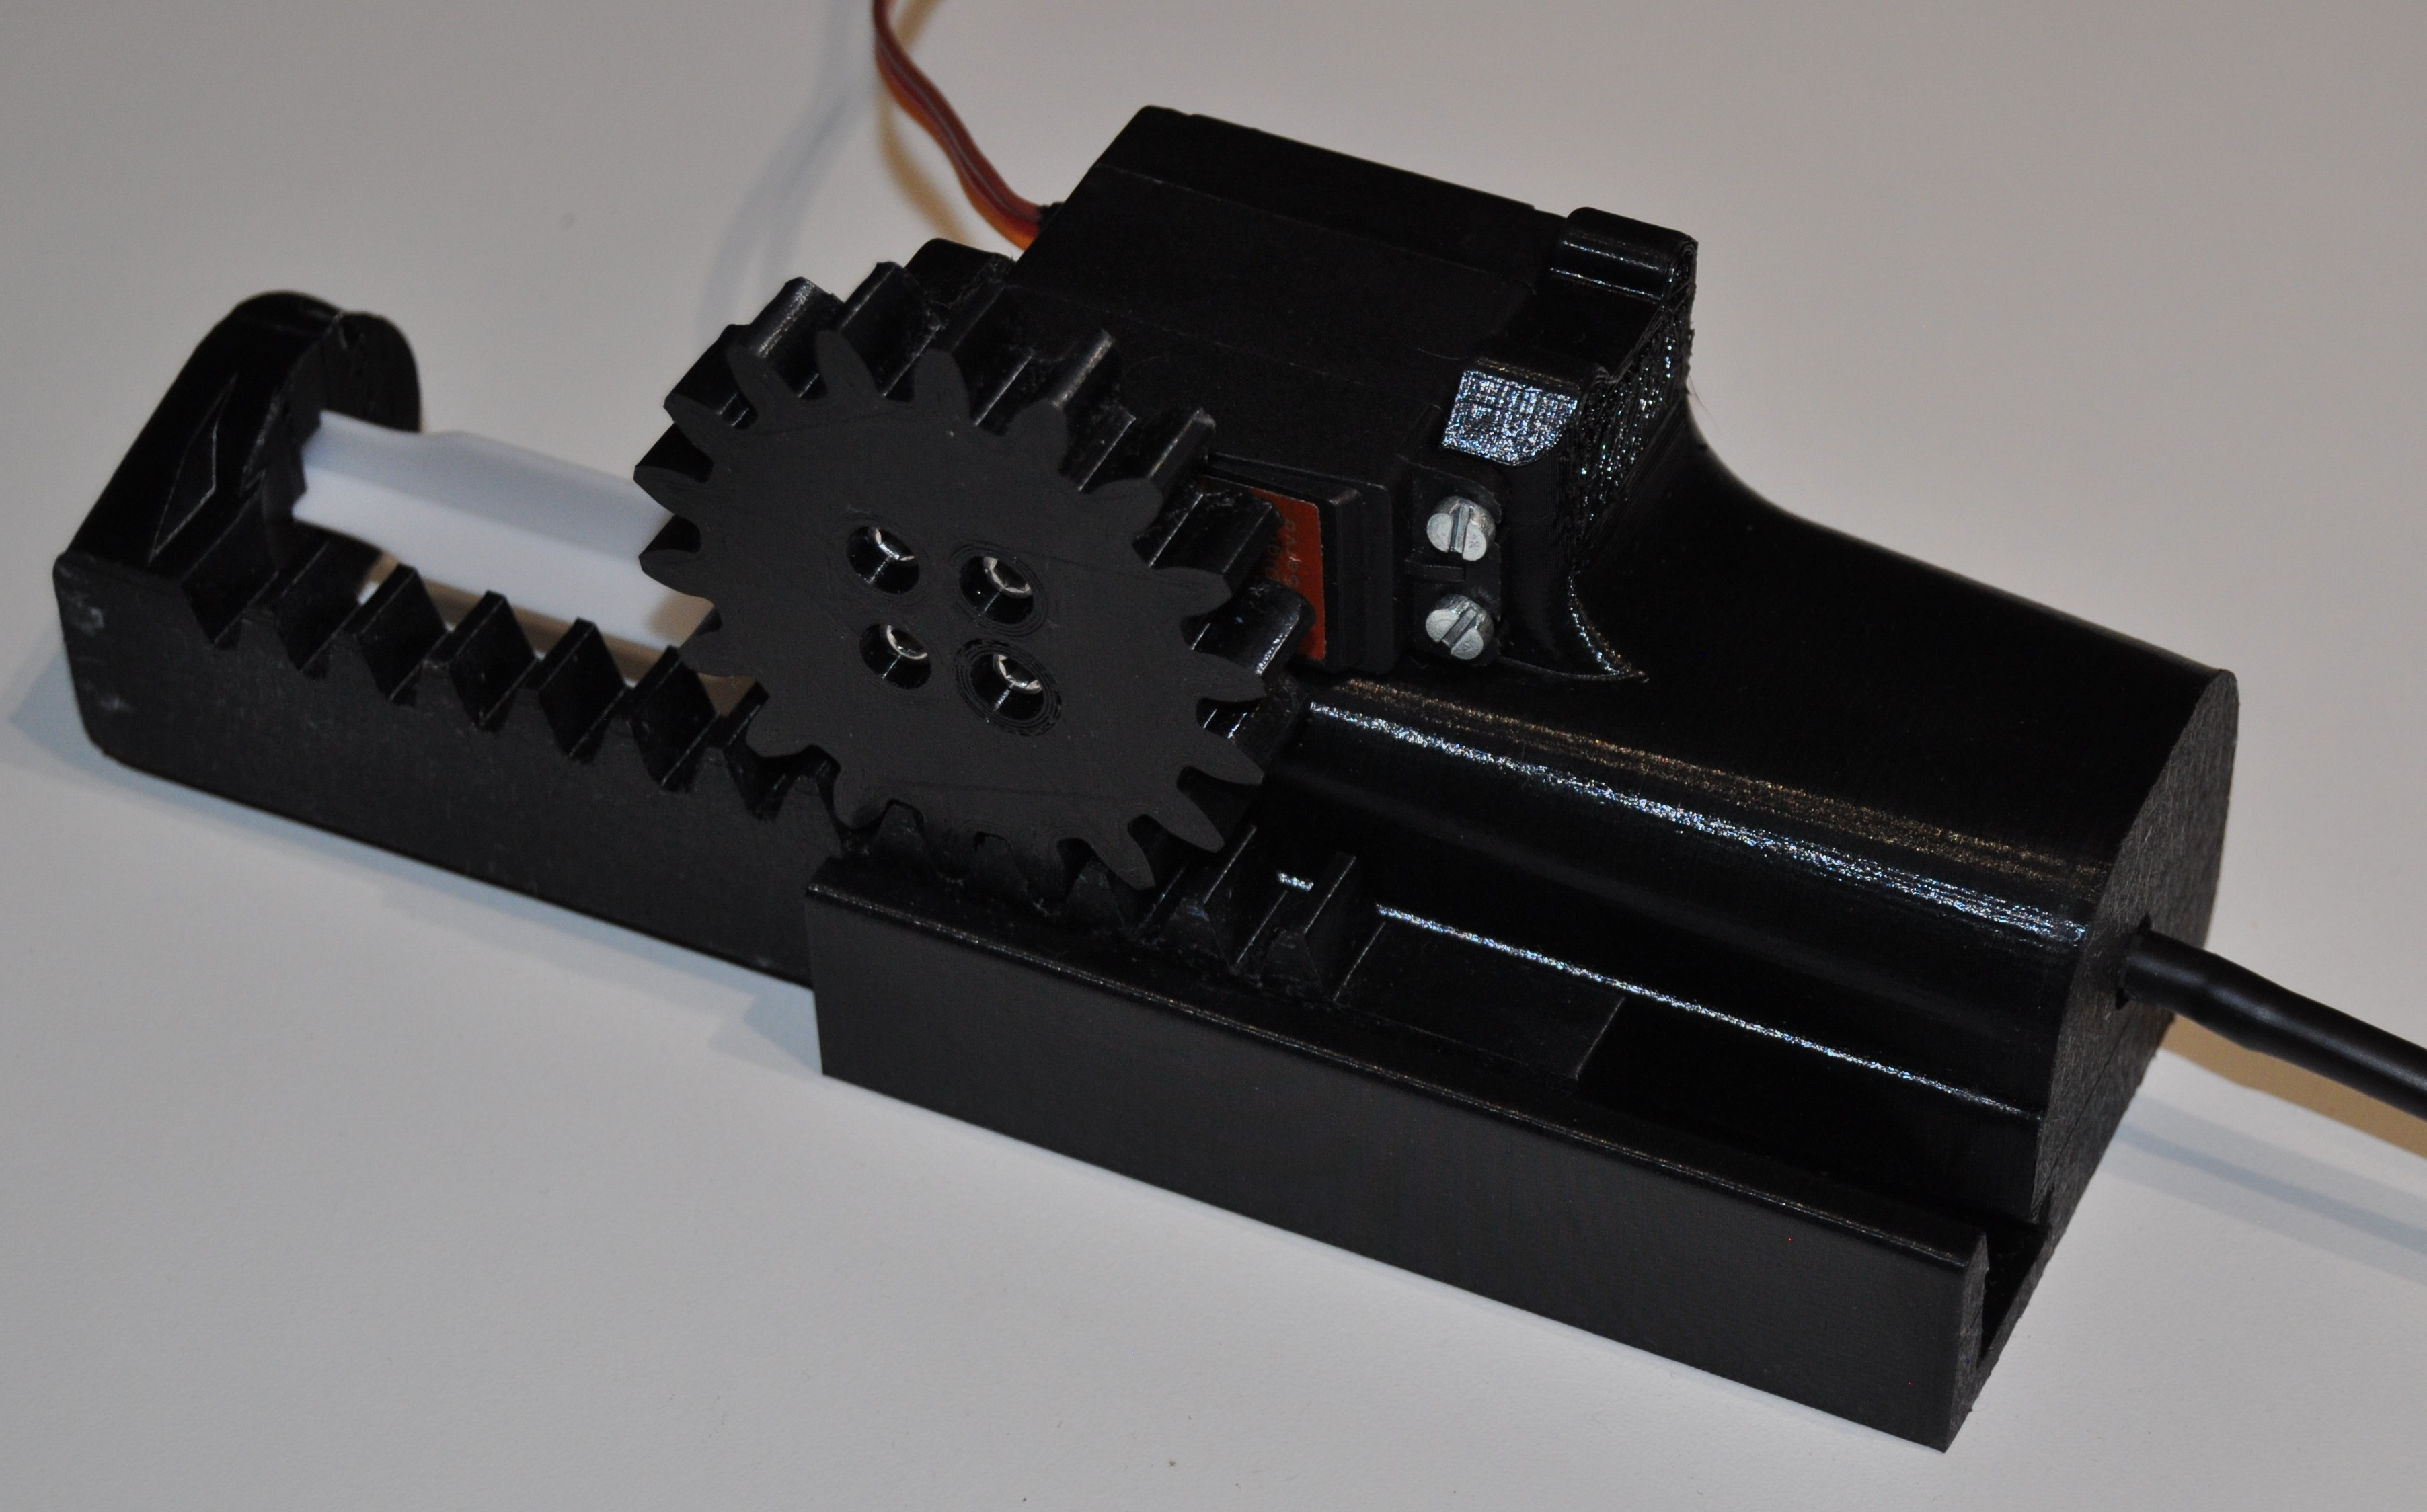
\includegraphics[width=0.6\linewidth]{figures/vacuum-actuator.JPG}
	\caption{Physical vacuum actuator model manufactured using 3D printing processes.}
	\label{fig:vacuum-actuator}
\end{figure}

\subsubsection{Robotic Manipulator}

The general motor-driven gantry robotic system design is currently the leading option for use in this project's solution. The reasons for this are as follows:

\begin{compactitem}
	\item A gantry-style robotic system offers the most structural stability due to the multiple mounting points for both the frame as well as the moving sub-components within the system. This mechanical stability improves the precision of the system which is one of the leading requirements in this application. It is for this reason that the gantry design is common in other high-precision applications such as pick-and-place operations in circuit manufacturing.
	\item Due to the Cartesian nature of the gantry movement, the precision of the system is relatively constant across all coordinates in the workspace. This stands in contrast to robotic arms which experience a deterioration in accurary as the distance from the robotic base increases.
	\item The frame of the gantry has the potential to include an integrated mount for the computer vision camera/s. This would allow the camera to always operate from a similar point relative to the workspace and reduce the inaccuracies that are introduced from positional shifts of the camera each time the system is used.
\end{compactitem}

\subsubsection{End-Effector Assembly}

The end-effector mount was designed to fulfil to following requirements:

\begin{compactitem}
	\item It must provide a mounting structure for both the 20BYGH406 stepper motor and the vacuum rod such that the gear components of each are aligned and able to mesh correctly.
	\item It must facilitate at least 5mm of translational motion of the vacuum rod along the z-axis.
	\item It must provide a connection point for connecting the end-effector mount to the rest of the robotic subsystem.
	\item It must facilitate assembly of the end-effector mount, 20BYGH406 stepper motor and vacuum rod components.
	\item It must be designed in such a manner that is amenable to being manufactured using and FDM 3D printing techniques. 
\end{compactitem}

Figure \ref{fig:end-effector-disassembled} shows the end-effector mount and supporting components that were designed to meet these requirements along with the 20BYGH406 stepper motor and vacuum rod. The end-effector mount, motor mount and vacuum rod top mound were originally designed as a single piece. The vacuum rod top mount was separated as a component to facilitate the insertion of the vacuum rod into the end-effector assembly. The motor mount was similarly separated to facilitate the manufacturing of this part using FDM 3D printing methods as the overhang was not capable of being printed without support. Figure \ref{fig:end-effector-assembled} shows the same components when assembled to form the complete end-effector mount assembly.

\begin{figure}[H]
	\centering
	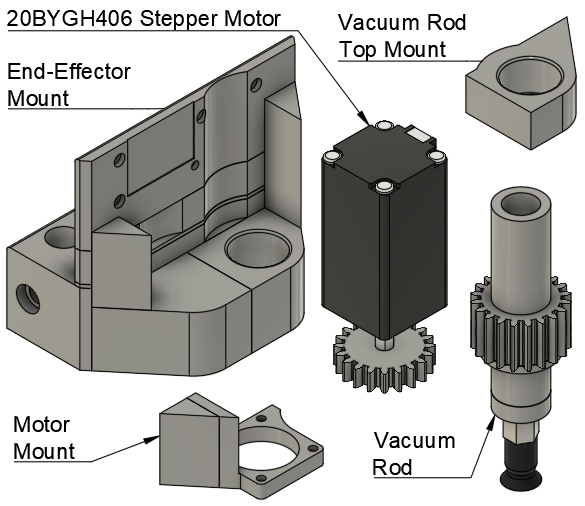
\includegraphics[width=0.6\linewidth]{figures/end-effector-disassembled.png}
	\caption{Disassembled end-effector mount assembly.}
	\label{fig:end-effector-disassembled}
\end{figure}

\begin{figure}[H]
	\centering
	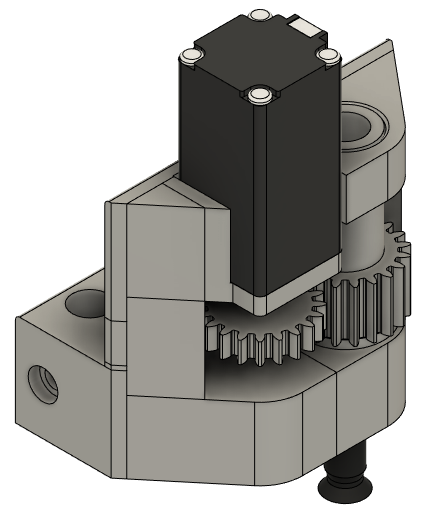
\includegraphics[width=0.3\linewidth]{figures/end-effector-assembled.png}
	\caption{Assembled end-effector mount assembly.}
	\label{fig:end-effector-assembled}
\end{figure}

\subsubsection{Z-Axis Assembly}

For the purposes of this project, the z-axis assembly is defined as the collection of mechanical components that move linearly along the z-axis when the z-axis drive mechanism is activated. In the case of this project, the z-axis drive mechanism is included in the z-axis assembly. There are many different approaches to the z-axis mechanism. One of the most common approaches which is often used in CNC applications involves the use of a linear guide which is fixed with respect to the motion of the z-axis assembly. The z-axis drive mechanism is also fixed with regards to the z-axis assembly. In other words, when the z-axis drive is activated, the z-axis assembly moves relative to the linear guides and the linear drive. The advantage of this approach is that the moving mass of the z-axis assembly is minimised as the linear guides and the z-axis drive mechanism are fixed relative to the motion. The linear bearings form part of the z-axis assembly in this case. The disadvantage of this approach is that a connecting component is required to connect the end-effector to the point at which the linear bearings connect to the linear guides. As such, the greater the range of motion along the z-axis that is required, the longer this connecting element has to be. This introduces a potential area of play as the connecting component is prone to a greater degree of flex the greater its length is. Therefore, this approach is only suited to tasks in which the range of motion along the z-axis is minimal.

Another variation of this approach is to include the linear guides as well as the z-axis drive as part of the z-axis assembly that moves along the z-axis. In this arrangement, the linear bearings are fixed with regards to the motion of the z-axis assembly. The disadvantage of this approach is that there is greater moving mass along the z-axis but this is allows a greater range of motion to be achieved along the z-axis. Since the nature of this project requires a reasonably large range of motion along the z-axis, this latter approach was selected.

With the approach including both the z-axis drive mechanism as well as the linear guides as part of the z-axis assembly, there are two primary design decisions. These are with regards to the selection of the linear guide components as well as the selection of the linear drive mechanism. The most popular drive mechanisms are the lead screw drive solution and the timing belt based drive mechanism. Timing belts are beneficial when the load needs to be moved over a relatively large distance at a relatively high speed. However, they generally require larger motors with more torque. Therefore, they are suited to motion along directions where they are not working against gravity. Lead screw drives, on the other hand, generally require small motors with less torque to drive the same load and are suited to moving loads slowly and accurately over small distances. Since the z-axis motor forms part of the moving z-axis assembly in the design approach discussed above, a smaller motor is preferable to reduce the moving mass of the assembly. Secondly, the range of motion along the z-axis is relatively small compared to the range of motion required along the x and y axes. Therefore a lead screw drive approach was selected for the z-axis assembly.

There are two popular linear guide mechanisms with regards to motion along the z-axis. The first is the linear rail guide which has excellent characteristics when it comes to resisting forces and torque in any other direction than its line of travel. Unfortunately, these preferable characteristics come at a cost. The linear rails in themselves are not completely stiff and need to be mounted to a supporting structure such as an aluminium v-slot extrusion which would increase the moving mass of the z-axis assembly to an unreasonable level. Secondly, the financial cost of the linear rails per relatively high. Therefore, linear rails were not selected for linear motion along the z-axis. Rather the alternative linear guide mechanism, namely linear rods, was selected instead. Specifically, 8mm diameter chromed steel linear rods were selected since they are one of smallest linear rod diameters available and the vertical nature of the z-axis assembly does not exert much torque on the linear rails.

Figure \ref{fig:end-effector-disassembled} shows that the end-effector mount already incorporates mounting points for the linear rods. A custom component needed to be designed to complete the z-axis assembly and needed to perform the following functions:

\begin{compactitem}
	\item It should provide a mounting location for the 35BYGH312P1 stepper motor in an orientation with the drive shaft at the bottom aligned with the z-axis.
	\item It should provide mounting points for the 8mm diameter linear chromed steel rods.
	\item It should provide a mounting point for the first line of the drag chain that will be used to route the cables for the 20BYGH406 stepper motor, the 35BYGH312P1 stepper motor and finally the vacuum tubing coming from the vacuum rod.
\end{compactitem}

Figure \ref{fig:z-axis-motor-mount} shows the component that was designed in order to meet these requirements. The component was designed in a such a manner that it is amenable to being manufactured using the process of FDM 3D printing with the use of supports for the overhang used to mount the drag chain link.

\begin{figure}[H]
	\centering
	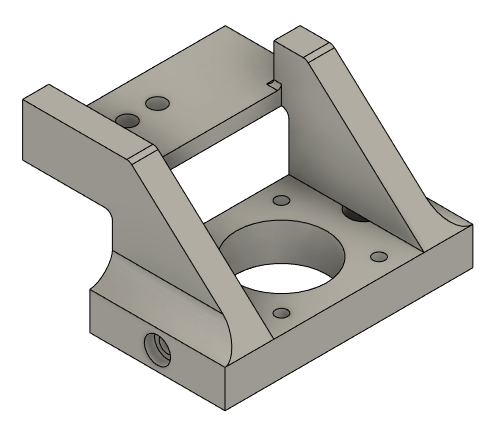
\includegraphics[width=0.4\linewidth]{figures/z-axis-motor-mount.png}
	\caption{Z-axis motor mount.}
	\label{fig:z-axis-motor-mount}
\end{figure}

The components that the z-axis assembly comprises of are summarised in the list below:

\begin{compactitem}
	\item End-effector mount assembly
	\item Z-axis motor mount
	\item 8mm diameter, 8mm pitch lead screw of length 168mm
	\item 8mm diameter to 5mm diameter rigid coupling to connect the lead screw to the shaft of the stepper motor
	\item 35BYGH312P1 stepper motor
	\item 2x 8mm diameter linear chromed steel rods of length 195mm
\end{compactitem}

Figure \ref{fig:z-axis-assembly} shows how all of these components are integrated to form the final z-axis assembly.

\begin{figure}[H]
	\centering
	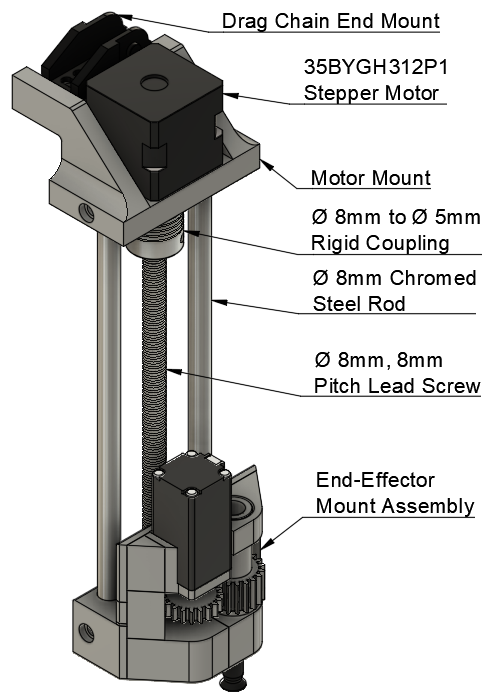
\includegraphics[width=0.6\linewidth]{figures/z-axis-assembly.png}
	\caption{Z-axis assembly.}
	\label{fig:z-axis-assembly}
\end{figure}

Z-Axis Mount

It was decided to use aluminium v-slot extrusions as the foundation of the robotic subsystem primarily due to the design flexibility offered this structure. The profile of the extrusion offers considerable stiffness required by the frame structure as well as mounting locations along any position of the structure by means of T-nuts. Furthermore, the v-shape present along the grooves in the extrusion allow the extrusion to be used as a linear guide. The extrusion was not considered as an option for a linear guide in the z-axis assembly due to its comparatively large mass compared to the mass of the z-assembly. However, in comparison to the mass of the x-axis assembly, the mass of the extrusion is much more reasonable and offers greater structural support in comparison to other linear guides such as linear chromed steel rods. The fact that the aluminium v-slot extrusion approach was selected for the rest of the robotic subsystem structure combined with the reasons discussed earlier was considered sufficient to select an aluminium extrusion as the x-axis linear guide. To assist in countering the torque generated about the x-axis by the z-axis assembly, it was decided to use a 2040 aluminium v-slot extrusion as opposed to a 2020 aluminium v-slot extrusion.

Linear motion along the aluminium v-slot extrusion is facilitated by v-slot wheels that run along the v-shaped grooves of the extrusion. Therefore, a need for a component to connect the z-axis assembly to the x-axis aluminium v-slot extrusion arose. The specific requirements of the required component are outlined below:

\begin{compactitem}
	\item The component needs to connect the 4 v-slot wheels positioned to run along the 2040 aluminium v-slot extrusion to the 4 linear bearings through which the linear chromed steel rods of the z-axis assembly run.
	\item The component needs to accommodate the excess movement required by the eccentric nuts used by half of the v-slot wheels.
	\item The component needs to provide mounting points for the timing belt on either side of the component.
	\item The component needs to provide a mounting point for the lead screw nut.
	\item The component needs to accommodate the length of the 8mm diameter to 5mm diameter rigid coupling used to attach the lead screw to the z-axis motor in the z-axis assembly. This accommodation allows the z-axis motor to move lower along the z-axis relative to the fixed linear bearings. This results in a shorter moment arm to the z-axis motor and reduces the torque about the x-axis.
	\item The component needs to be capable of being manufactured using FDM 3D printing techniques.
	\item The component needs to support assembly with all of its supporting components.
\end{compactitem}

\begin{figure}[H]
	\centering
	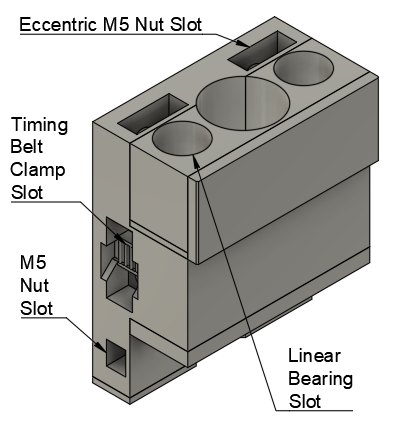
\includegraphics[width=0.35\linewidth]{figures/z-axis-mount.png}
	\caption{Z-axis mount component for the z-axis assembly without supporting components.}
	\label{fig:z-axis-mount}
\end{figure}

Figure \ref{fig:z-axis-mount} shows the z-axis mount developed to meet these requirements with various design features relating to these requirements highlighted. The walls of the eccentric spacer measure 1.76 mm and 0.34 mm. That means the bolt may be offset a maximum of 0.71 mm in any direction from the centre of the outer radius of the eccentric spacer which is accommodated in the design by the feature identified as the eccentric M5 nut slot.

The following components are used in conjunction with the z-axis mount:

\begin{compactitem}
	\item 4x delrin solid v-wheels
	\item 4x LM8UU linear bearings
	\item 8mm pitch delrin lead screw nut
	\item 2x eccentric nuts for v-wheels
	\item 4x M5x30 DIN 84 slotted cheese head machine screws
	\item 4x M5 washers
	\item 2x custom designed timing belt clamps
\end{compactitem}

Figure \ref{fig:z-axis-mount-assembled} shows the z-axis mount assembled with all the components listed above is shown from an angled perspective from below the component. The 8mm pitch lead screw nut can be seen centred near the bottom of the component. One of the timing belt clamps can be seen placed over the timing belt clamp slot on the side of the z-axis mount.

\begin{figure}[H]
	\centering
	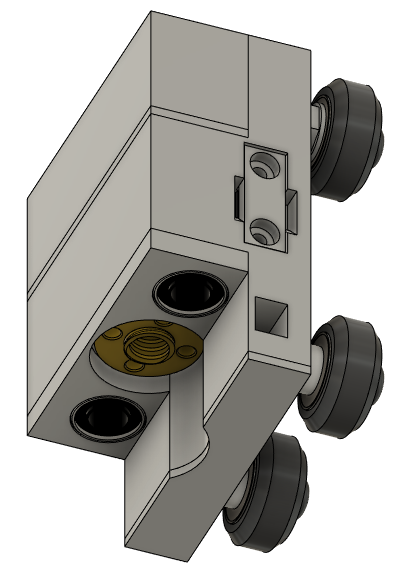
\includegraphics[width=0.3\linewidth]{figures/z-axis-mount-assembled.png}
	\caption{Z-axis mount component for the z-axis assembly with supporting components.}
	\label{fig:z-axis-mount-assembled}
\end{figure}

\subsubsection{X-Axis Assembly}

For the purposes of this project, the x-axis assembly is defined in a similar manner to the z-axis assembly. Specifically, the x-axis assembly is the collection of components that move linearly along the x-axis when the x-axis drive motor is activated. Similar to the z-axis assembly, a decision needs to be made regarding whether to position the x-axis drive motor as part of the x-axis assembly or not. There is no significant benefit to including the x-axis motor as part of the x-axis assembly either than it potentially reduces the complexity of the x-axis mount which no longer needs to support the motor as well. However, this is offset by the complexity increase in the z-axis mount which would need to include a mounting point for the x-axis motor. Furthermore, mounting the motor in this manner would increase the mass of the x-axis assembly which would require a larger motor with more torque to drive. For these reasons, it was selected to not include the x-axis motor in the x-axis assembly. Note, the x-axis assembly does not include the x-axis linear guide in the form of the 2040 aluminium v-slot extrusion as it does not move when the x-axis drive is activated.

The second design consideration is the selection of the drive mechanism. Again, a lead screw approach was considered against a timing belt based approach. In this situation, the drive mechanism does not need to work directly against gravity as was the case with z-axis assembly. Furthermore, the range of motion of the x-axis assembly is significantly greater than that of the z-axis assembly. Based on these factors, in conjunction with the discussion of the drive mechanisms covered during the z-axis assembly analysis, the timing belt approach was selected. Due to the existence of the v-wheels to connect the z-axis mount to the aluminium extrusion, it was identified as being significantly more complicated to route the timing belt with the flat face parallel to the base plane. However, there were no obvious restrictions in routing the timing belt with the front face parallel to the x-axis aluminium v-slot extrusion. Furthermore, the aluminium v-slot extrusion facilitates the routing of the far side of the belt through the centre of the extrusion. For these reasons, it was decided to route the timing belt in this manner. Therefore, with all of the above considered, the x-axis assembly is defined to only consist of the z-axis mount as well as the z-axis assembly. Figure \ref{fig:x-axis-assembly} shows x-axis assembly positioned on the x-axis aluminium v-slot extrusion.

\begin{figure}[H]
	\centering
	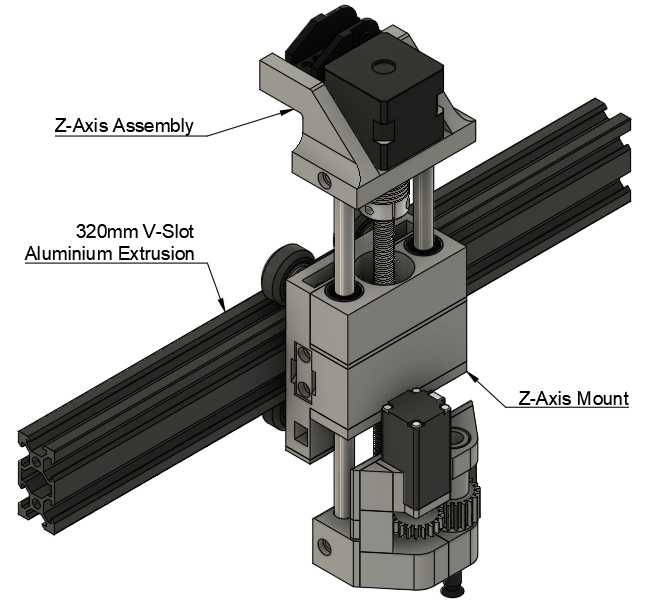
\includegraphics[width=0.8\linewidth]{figures/x-axis-assembly.png}
	\caption{X-axis assembly consisting of the z-axis mount supporting the z-axis assembly.}
	\label{fig:x-axis-assembly}
\end{figure}

\subsubsection{Y-Axis Assembly}

For the purposes of this project, the y-axis assembly is defined in a similar manner to the z-axis and x-axis assemblies. Specifically, the y-axis assembly is the collection of components that moves linearly along the y-axis when the y-axis drive is activated. At this point in the design, the x-axis assembly is the highest level component of the robotic subsystem. The x-axis assembly runs along the x-axis aluminium v-slot extrusion. In order to introduce linear motion along the y-axis, both of these components need to be translated and therefore will both form part of the y-axis assembly.

In order to facilitate linear motion along the y-axis, linear guides need to be introduced into the design. Again, the most popular two linear guides were considered, namely the linear rail and the linear chromed steel rod. A consideration that applies to the y-axis motion that did not apply to the linear guides used on the other axes is the fact that the y-axis linear guides will always be fixed relative to the robotic structure. Therefore, weight is not a consideration in the selection of the linear guides. Furthermore, it has already been noted that aluminium v-slot extrusions are used to form the frame of the robotic subsystem. These extrusions facilitate simple mounting of linear rails by means of T-nuts. Furthermore, all of the mechanical advantages of the linear rail over the linear chromed steel rod as discussed earlier still apply. Since the y-axis assembly has the greatest mass of any of the moving components, the mechanical advantages offered by the linear rail were considered more relevant here than in earlier parts of the design. V-wheels were also considered as a means of linear motion along the v-slot aluminium extrusion. However, exploration of potential designs using this mechanisms exhibited many issues with routing the timing belt for the x-axis as well as the y-axis. Furthermore, the aluminium spacers would introduce additional length along the x-axis without any increase in the range of motion along the x-axis. 

For these reasons, the linear rail was selected as the linear guide along the y-axis. Furthermore, since both sides of the x-axis aluminium v-slot extrusion need to be supported, it was decided to use two linear rails, one on either side of the x-axis aluminium extrusion. The MGN12H linear bearing acts as the connection between the linear rail and the load item. Therefore, a requirement for two components to connect both ends of the x-axis aluminium extrusion to the MGN12H bearings arose. The requirements of the first component are as follows:

\begin{compactitem}
	\item The component needs to connect the left side of the x-axis 2040 aluminium v-slot extrusion to the left MGN12H linear bearing.
	\item The component needs to provide a mounting point for the 42BYGHW609 stepper motor such that the motor is in a position to drive the x-axis timing belt.
	\item The component needs to provide a timing belt clamping point on both sides of the component for the left y-axis timing belt.
	\item The component needs to facilitate the routing of the x-axis timing belt.
	\item The item needs to provide a mounting point for the end piece of the drag chain to facilitate the routing of wires and tubing originating from the z-axis assembly as well as the 42BYGHW609 stepper motor cables.
	\item The component needs to be capable of being manufactured using FDM 3D printing techniques.
\end{compactitem}

Figure \ref{fig:x-axis-mount-left} shows the left x-axis mount that was designed to meet these requirements along with indications of the roles of the various parts of the design. Similarly, the requirements of the second component are:

\begin{compactitem}
	\item The component needs to connect the right side of the x-axis 2040 aluminium v-slot extrusion to the right MGN12H linear bearing.
	\item The component needs to provide a mounting point for an idler pulley for a 6mm timing.
	\item The component needs to facilitate the movement of the idler pulley along the x-axis to allow the x-axis timing belt to be adjusted to the correct tension.
	\item The component needs to provide a timing belt clamping point on both sides of the component for the right y-axis timing belt.
	\item The component needs to facilitate the routing of the x-axis timing belt.
	\item The component needs to be capable of being manufactured using FDM 3D printing techniques.
\end{compactitem}

Figure \ref{fig:x-axis-mount-right} shows the right x-axis mount that was designed to meet these requirements along with indications of the roles of the various parts of the design.

\begin{figure}[H]
	\centering
	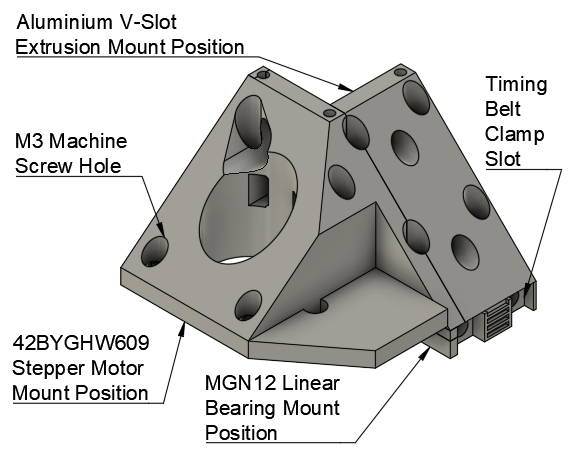
\includegraphics[width=0.45\linewidth]{figures/x-axis-mount-left.png}
	\caption{X-axis assembly left mount.}
	\label{fig:x-axis-mount-left}
\end{figure}

\begin{figure}[H]
	\centering
	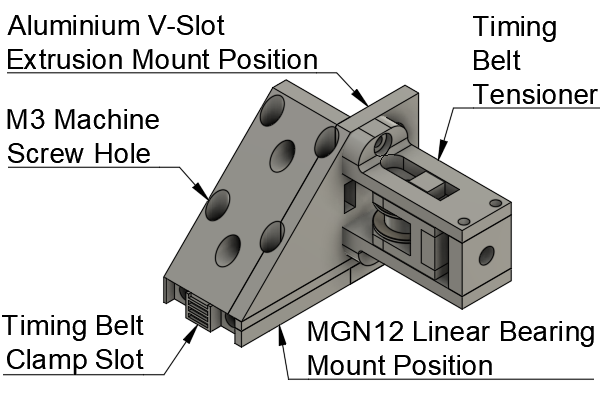
\includegraphics[width=0.4\linewidth]{figures/x-axis-mount-right.png}
	\caption{X-axis assembly right mount.}
	\label{fig:x-axis-mount-right}
\end{figure}

The components that comprise the y-axis assembly are as follows:

\begin{compactitem}
	\item X-axis assembly
	\item X-axis 2040 aluminium v-slot extrusion of length 320mm
	\item Left x-axis mount
	\item Right x-axis mount
	\item 2x MGN12H linear bearings
	\item 42BYGHW609 stepper motor
	\item 4x custom timing belt clamps
	\item 20 tooth GT2 pulley for GT2 timing belt
	\item Idler pulley for 6mm belt
\end{compactitem}

\subsubsection{Final Assembly}

The highest level component of the robotic subsystem at this point in the design is the y-axis assembly. In order to complete the design, several components still need to be developed, namely the belt tensioners to be used on both the left and right y-axis timing belts as well as the y-axis drive mechanism. The y-axis belt tensioners have identical functions with the only difference being their operation on opposite sides of the robotic subsystem. Therefore, the left and right y-axis timing belt tensioners are mirror images of each other and essentially share the same design. The y-axis belt tensioner component needs to meet the following requirements.

\begin{compactitem}
	\item The component needs to provide a mounting point for the idler pulley for a 6mm timing belt.
	\item The component needs to facilitate mounting of itself to the aluminium v-slot frame of the robotic subsystem.
	\item The component needs to facilitate adjustment of the position of the idler pulley along the y-axis to allow the tension of the y-axis timing belt to be adjusted.
	\item The component needs to be capable of being manufactured using FDM 3D printing techniques.
\end{compactitem}

Figure \ref{fig:y-axis-belt-tensioner-right} shows the y-axis belt tensioner that was designed to fulfil these requirements on the right side of the robotic subsystem.

\begin{figure}[H]
	\centering
	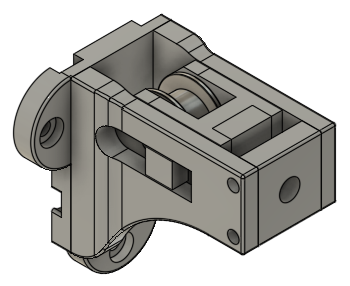
\includegraphics[width=0.4\linewidth]{figures/y-axis-belt-tensioner-right.png}
	\caption{Y-axis belt tensioner for the right drive side.}
	\label{fig:y-axis-belt-tensioner-right}
\end{figure}

The second design that needs to be completed in order to complete the robotic subsystem is the y-axis drive mechanism. The primary requirement of this mechanism is that it needs to be capable of driving the y-axis timing belts on both the left and right side of the robotic subsystem. The obvious basis of this mechanism is to use a dual shaft stepper motor with each shaft used to drive one of the y-axis timing belts. The 42BYGHW920L21B2 stepper motor was selected for this characteristic. Unfortunately, the length of the stepper motor is not sufficient to drive each belt directly off each shaft. Instead it was decided to drive only the left side y-axis timing belt directly off the shaft using a 20 tooth pulley for a 6mm GT2 timing belt with a 5mm bore. In order to drive the right side y-axis timing belt, the torque needs to be transferred from the stepper motor shaft to a pulley connected to the timing belt. It was decided to use an 8mm linear chromed steel rod in order to transfer this torque to a 20 tooth pulley for a 6mm GT2 timing belt with a 8mm bore. An 8mm diameter to 5mm diameter coupling is required to connect the stepper motor shaft to the 8mm linear rod. The rigid coupling is not sufficient to support the linear rod along the drive axis. Therefore, two KP08 8mm pillow block bearings were introduced to support the linear rod. In order to connect the pillow blocks to the aluminium v-slot extrusion frame of the robotic subsystem, two custom connector components needed to be designed. Similarly, a component needed to be designed to connect the 42BYGHW920L21B2 stepper motor to the frame as well. All of the components discussed above form the y-axis drive mechanism which is shown attached to the robotic subsystem in Figure \ref{fig:y-axis-drive-assembly}. The final robotic subsystem assembly is shown in Figure \ref{fig:final-assembly}.

\begin{figure}[H]
	\centering
	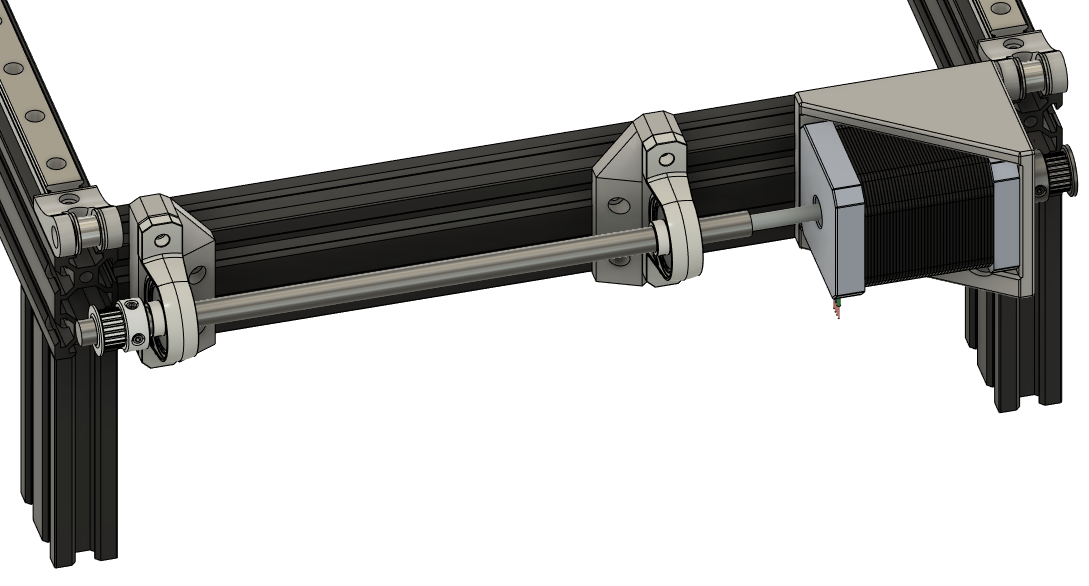
\includegraphics[width=0.7\linewidth]{figures/y-axis-drive-assembly.png}
	\caption{Y-axis drive assembly.}
	\label{fig:y-axis-drive-assembly}
\end{figure}

\begin{figure}[H]
	\centering
	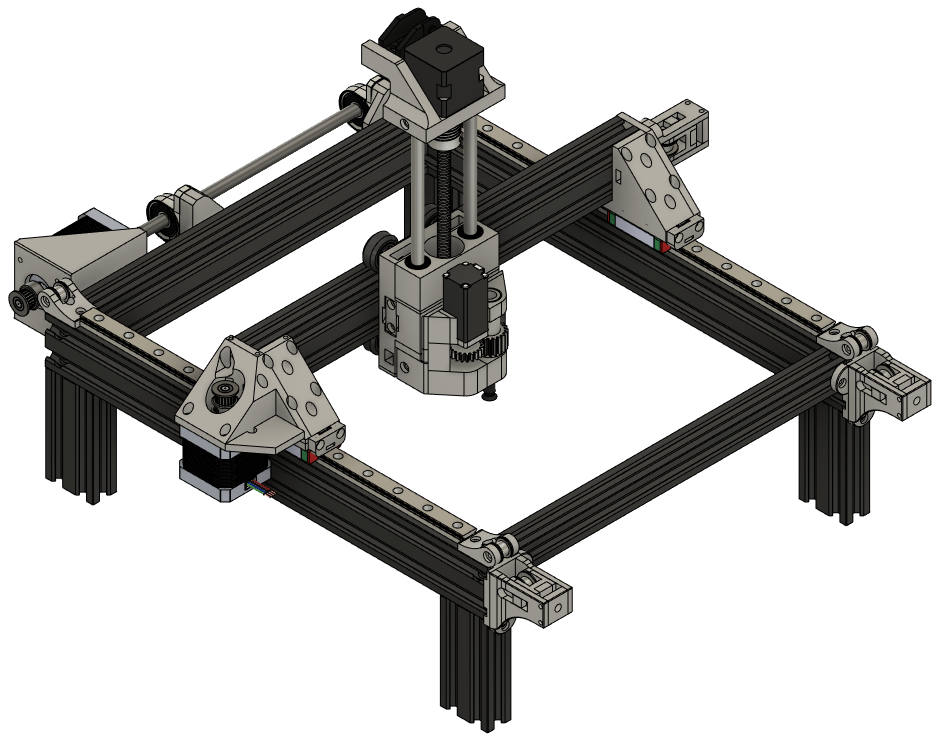
\includegraphics[width=0.9\linewidth]{figures/final-assembly.png}
	\caption{Final robotic subsystem assembly.}
	\label{fig:final-assembly}
\end{figure}

%Component Manufacturing
%
%I have a personal 3D printer available and therefore it was decided to manufacture the custom components designed for the robotic subsystem using this 3D printer. One of the most commonly used filaments for 3D printing is PLA primarily due to the fact that it is easier to print. However, PLA has a low glass transition temperature of $50^{\circ}C$. This means that it is possible for the plastic to soften if left in direct sunlight. For this and other reasons, PLA is usually used for art prints as opposed to engineering prints. A filament more suited to engineering applications is PETG. PETG has a higher glass transition temperature of $80^{\circ}C$ which is much better suited to everyday conditions. Furthermore, PETG has mechanical properties that make it less likely to mechanically fail than PLA. Therefore, it was chosen to use PETG to manufacture the custom components using FDM 3D printing techniques. PETG has the drawback that it is more challenging to print than PLA. In order to achieve successful prints, all of the custom components were printed using a build plate temperature of $85^{\circ}C$ and a nozzle temperature of $240^{\circ}C$. Furthermore, blue painters tape was first placed on the glass build plate to improve build plate adhesion along with rafts. However, the rafts needed to be manually cut away after the print had completed while the blue painter's tape had to be softened by soaking in IPA alcohol before being removed. Figure \ref{fig:3d-printed-components} shows all of the custom components printed using the method described over the course of approximately one week. The majority of the components were printed using 0.12 mm layer height to best capture the intricate part details.
%
%\begin{figure}[H]
%	\centering
%	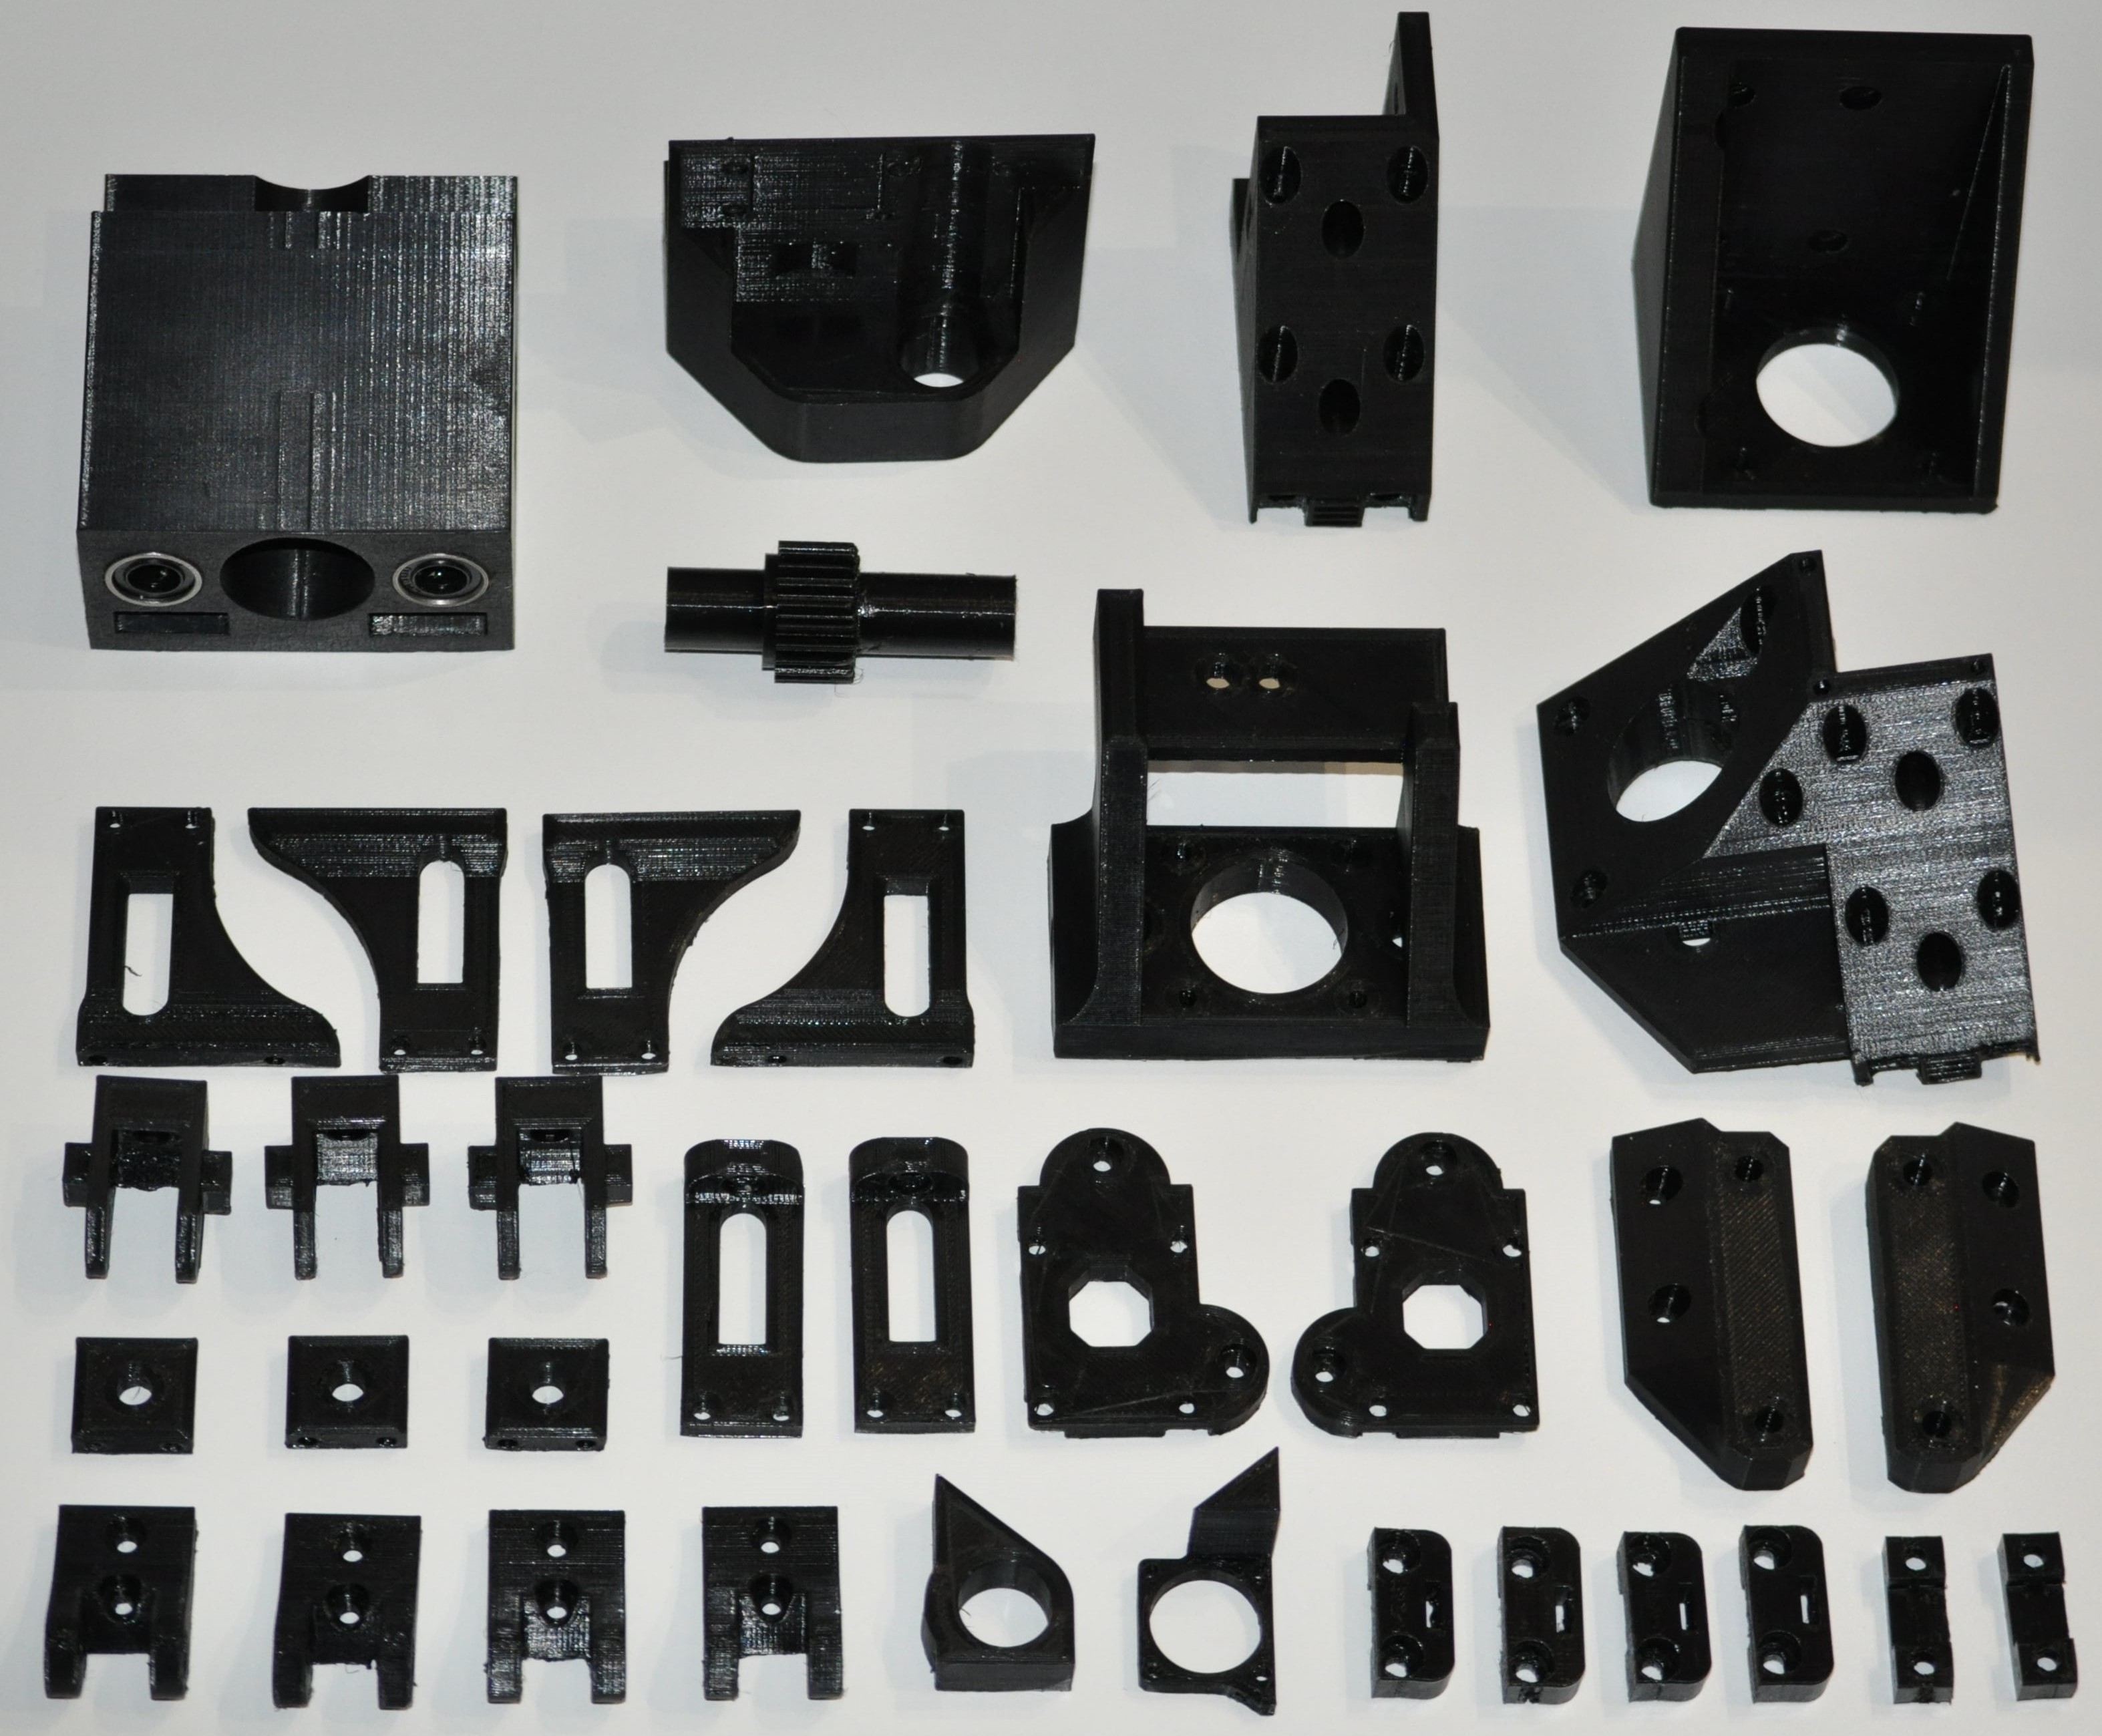
\includegraphics[width=0.7\linewidth]{figures/3d-printed-components.JPG}
%	\caption{All the robotic components that were manufactured by means of FDM 3D printing methods.}
%	\label{fig:3d-printed-components}
%\end{figure}
%
%Metal Component Machining
%
%A number of metal components including aluminium v-slot extrusions, chromed steel linear rods, linear rails and a stainless steel leadscrew were required in order to construct the robotic subsystem. These components could only be purchased in set lengths and therefore needed to be cut to the correct length for the project. Since the length of components such as the y-axis rail spacer extrusions and the leg extrusions affected the accuracy of the robotic subsystem (in terms of consistency of height and distance between the linear rails), the components needed very close to their design length. Therefore, a tolerance of 0.1 mm for the component lengths was specified. Furthermore, in order to facilitate the joining of aluminium extrusions in the design, M5 threads of 20mm depth needed to be tapped into the ends of some of the aluminium extrusions. M5 clearance holes also needed to be drilled through the extrusions along with the corresponding counterbores. Again the tolerance specified for this was 0.1 mm. The high accuracy required for these tasks required specialised machinery. In order to acquire access to such machinery, I approached the Heavy Machinery Lab at the University of Pretoria and was able to acquire access to use the machinery.
%
%The following list summarises the structural components as procured as well as the lengths each of the original components needed to be cut into:
%
%\begin{compactitem}
%	\item 1m 2040 aluminium v-slot extrusion: Cut into 3 x 80mm and 2 x 370mm lengths
%	\item 1m 2040 aluminium v-slot extrusion: Cut into 1 x 80mm, 1 x 280mm and 1 x 320mm lengths
%	\item 1m 2020 aluminium v-slot extrusion: Cut into 2 x 250mm and 1 x 370mm lengths
%	\item 1m 2020 aluminium v-slot extrusion: Cut to length 280mm
%	\item 1m 8mm diameter chromed steel rod: Cut into 2 x 195mm and 1 x 213mm lengths
%	\item 1m, 12mm x 8mm, stainless steel linear rail: Cut into 2 x 320mm lengths
%	\item 300mm 8mm diameter stainless steel lead screw: Cut to length 168mm
%\end{compactitem}
%
%\begin{figure}[H]
%	\centering
%	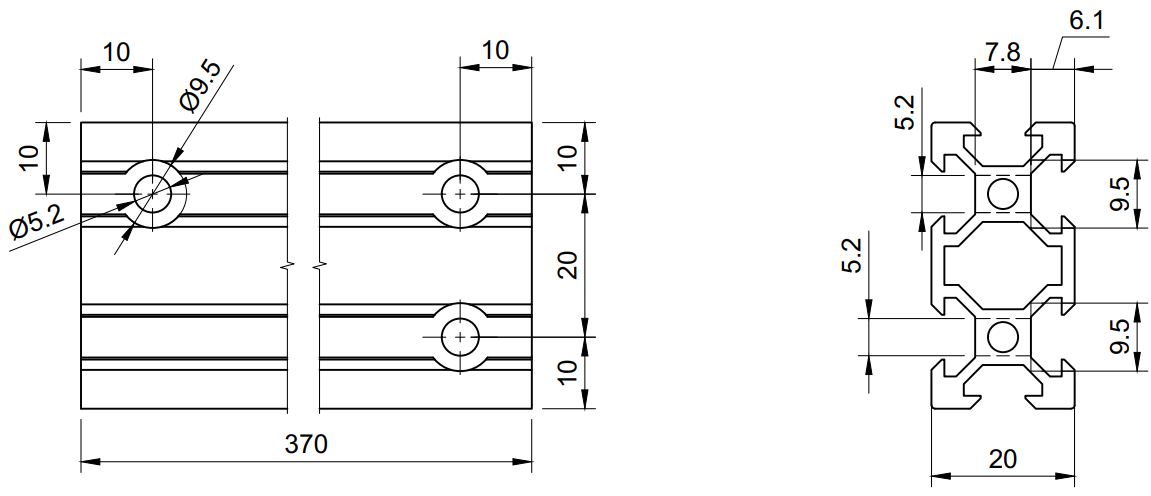
\includegraphics[width=0.7\linewidth]{figures/hg2-001-drawing.png}
%	\caption{Technical drawing showing the M5 clearance holes to be cut into the left y-axis 2040 aluminium v-slot extrusion.}
%	\label{fig:hg2-001-drawing}
%\end{figure}
%
%In order to cut the components to the correct length, a bandsaw to cut the component with approximately 1 mm excess. The bandsaw does not produce a perfectly straight or square cut and the tolerance is relatively high. In order to attain the 0.1 mm tolerance specification, the milling machine was used to shave the excess material of the face of the component to an accuracy of approximately 10 microns. Figure\ ref{fig:hg2-001-drawing} and Figure \ref{fig:hg2-002-drawing} show the technical drawings for the M5 clearance holes that needed to be cut into the y-axis extrusions to facilitate joining of the components to the frame. The drawings were created to be sent in for review during the application process to access the Heavy Machinery Lab. Across the course of three days in the Heavy Machinery Lab, all the required tasks were completed barring the length milling of 6 of the extrusions. It is estimated this will take another day to complete subject to the demand of the milling machine. Figure \ref{fig:machined-components} shows the current state of the machined components.
%
%\begin{figure}[H]
%	\centering
%	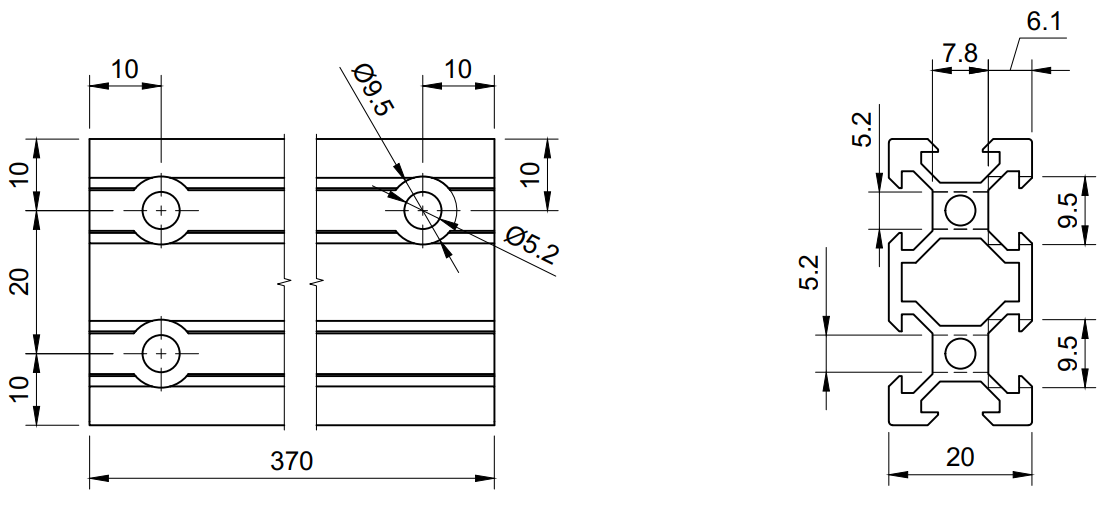
\includegraphics[width=0.7\linewidth]{figures/hg2-002-drawing.png}
%	\caption{Technical drawing showing the M5 clearance holes to be cut into the right y-axis 2040 aluminium v-slot extrusion.}
%	\label{fig:hg2-002-drawing}
%\end{figure}
%
%\begin{figure}[H]
%	\centering
%	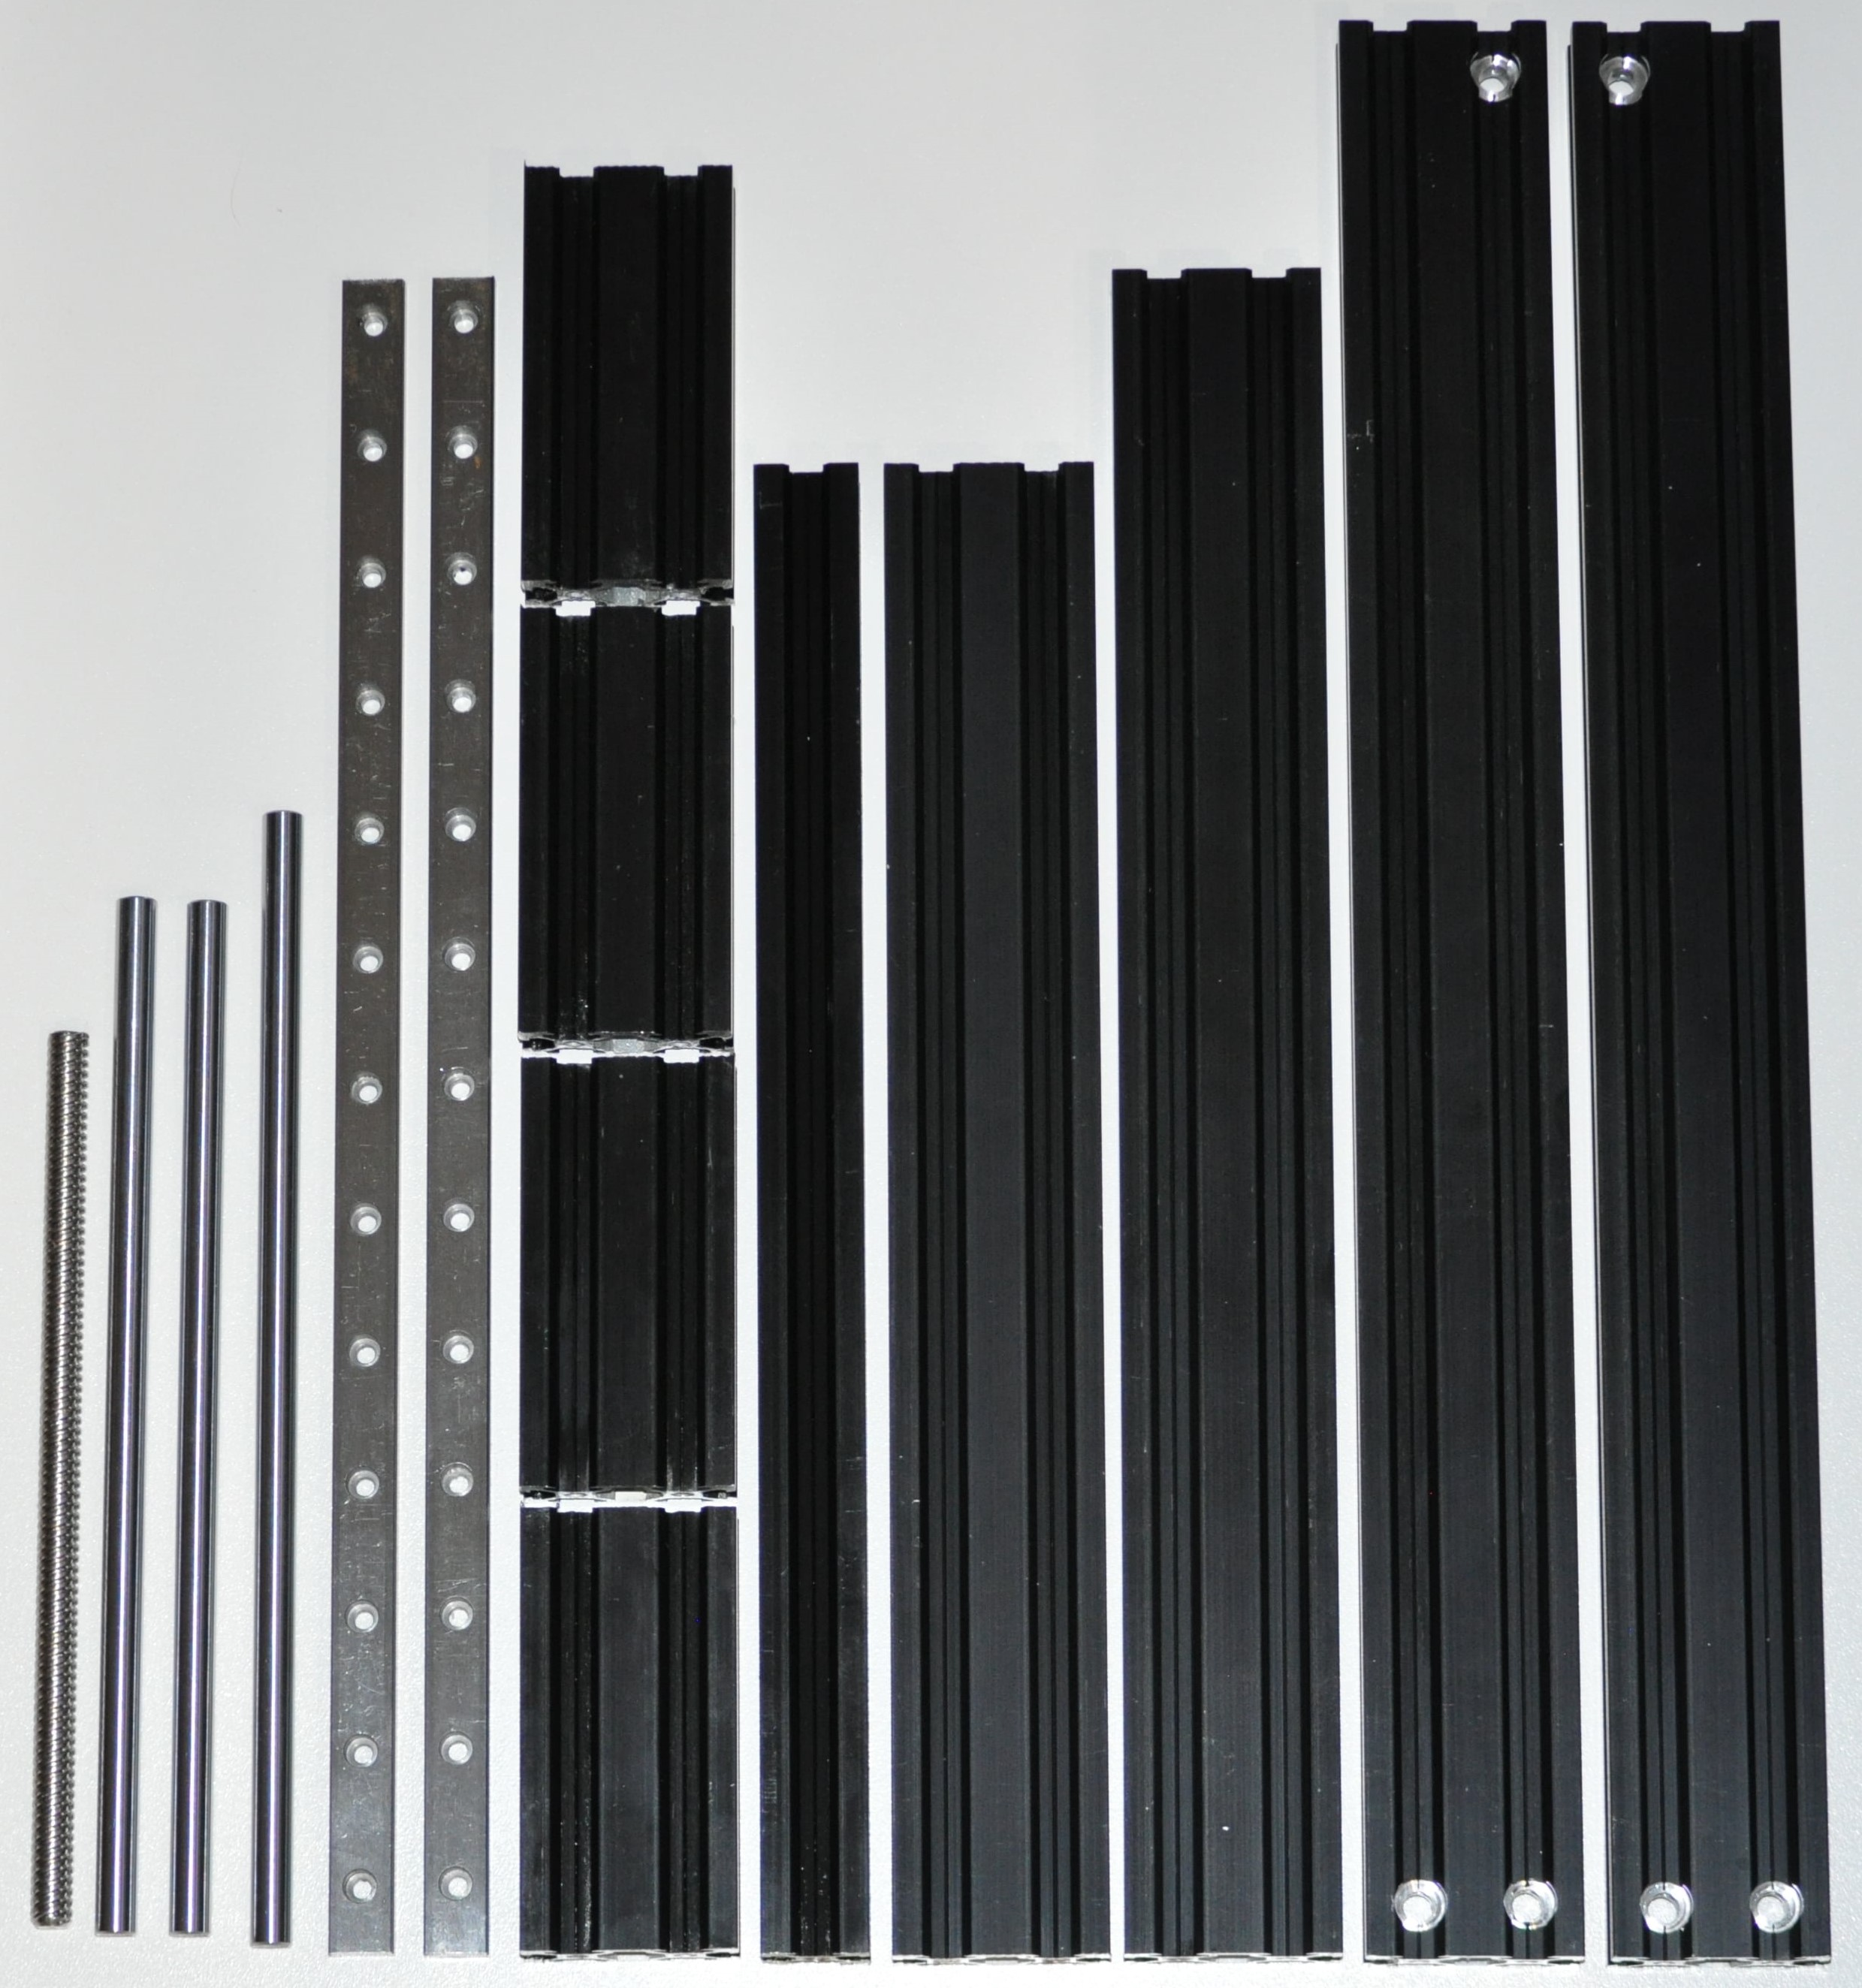
\includegraphics[width=0.5\linewidth]{figures/machined-components.JPG}
%	\caption{Metal components after the machining process.}
%	\label{fig:machined-components}
%\end{figure}

\subsection{Embedded Robot Controller} \label{sec:Embedded Robot Controller}

The \textit{Robotic System} required an embedded controller to drive the end-effector mechanism and the robotic manipulator developed as part of the mechanical robotic component in Section \ref{sec:Mechancial Robotic Component} as well as to facilitate communication with the \textit{PC System}. Specifically, in service of these requirements, the embedded controller needed to fulfill the following functions:

\begin{compactitem}
	\item The controller should provide control signals to control the four robotic manipulator stepper motors as well as the vacuum mechanism servo motor.
	\item The controller should capture the pressure sensor reading in the vacuum system.
	\item The controller should facilitate bi-directional communication with the \textit{PC System} such that the \textit{PC System} can send control commands to and receive status information from the \textit{Robotic Subsystem}.
	\item The controller should distribute energy from a power supply to the components in the \item Robotic System including the stepper motors, servo motor, cooling fan (for the embedded controller) and robot workspace lights.
	\item The controller should monitor the robotic manipulator limit switches on each Cartesian axis.
\end{compactitem}

The hardware considerations of the circuit designed to fulfill these requirements are outlined in Section \ref{sec:Circuit Design} while the development of the physical realisation of this circuit in the form of a printed circuit board (PCB) is presented in Section \ref{sec:PCB Design}. Following this, the firmware implementations developed to fulfill various facets of the embedded controller's functional requirements are discussed.

\subsubsection{Circuit Design} \label{sec:Circuit Design}

As noted in the project proposal, the motor drivers for the robotic manipulator stepper motors were taken off-the-shelf. The DRV8825 stepper motor driver was selected for this purpose since the driver is capable of supplying up to 1.5 A to the motor which is sufficient for the selected robotic manipulator motors. Specifically, the DRV8825 driver breakout board was selected for use in this project. Each DRV8825 driver exposes four output drive pins to control the current in both coils in the connected stepper motor. Furthermore, the DRV8825 driver exposes a number of input pins to control the operation of the motor and the driver.

The DRV8825 driver control inputs and status outputs of interest for this project are shown in Table \ref{tab:drv8825-input-pins} and their use in this project is detailed in Section \ref{sec:Motor Control}. Therefore, the microcontroller around which the embedded controller is based needs to provide seven digital output pins and one digital input pin is per stepper motor. Furthermore, the STEP pin needs to be controlled with time-sensitive signals and as such one timer peripheral is required for each stepper motor. Since the robotic manipulator makes use of four stepper motors, a total of 28 digital output pins, four digital input pins and four timer peripherals are required in the microcontroller to control the motors.

\begin{table}[H]
	\renewcommand{\arraystretch}{1.3}
	\centering
	\begin{tabular}{|>{\raggedright}m{1.5cm}|>{\raggedright}m{2.3cm}|>{\raggedright}m{1.5cm}|>{\raggedright\arraybackslash}m{8cm}|}
		\hline
		\textbf{Pin No.} & \textbf{Pin Name(s)} & \textbf{Type} & \textbf{Description} \\
		\hline
		2,3,4 & M0, M1, M2 & Input & Microstepping resolution selection \\
		\hline
		5 & $\overline{\text{RESET}}$ & Input & Reset the driver's step indexer \\
		\hline
		6 & $\overline{\text{SLEEP}}$ & Input & Place the motor in a low-power sleep state \\
		\hline
		7 & STEP & Input & Motor rotation direction selection \\
		\hline
		8 & DIR & Input & Advance the motor one step on rising edge \\
		\hline
		10 & $\overline{\text{FAULT}}$ & Output & Overheat and overcurrent event flag \\
		\hline
	\end{tabular}
	\caption[Caption for LOF]{\label{tab:drv8825-input-pins}DRV8825 breakout board control and status pins.\footnotemark}
\end{table}

\footnotetext{The overline notation, $\overline{\text{PIN}}$, on a pin name indicates the control input or status output is active low.}

In order to facilitate serial communication with the \textit{PC Subsystem}, the UART protocol was selected as the basis for this communication. The selection was made as the communication with the \textit{PC System} was expected to only consist of simple asynchronous control commands and status updates which are easily supported by UART. The universal serial bus (USB) interface of the \textit{PC System} is not directly compatible with the UART serial interface peripheral and, as such, the CH340G IC was selected as the communication data conversion point between these two interfaces. The CH340G exposes a transmitter (TX) pin and receiver (RX) pin for the microcontroller to interface with. Therefore, the microcontroller requires one digital input pin, one digital output pin and a UART peripheral to support serial communication. The serial communication component is discussed further in Section \ref{sec:Serial Communication}

In addition to the stepper motor and UART control pins, a single digital output pin was required to control the vacuum system servo motor along with a timer peripheral to act as the time base for the pulse width modulation (PWM) signal. An analog input pin, in conjunction with a corresponding analog-to-digital converter (ADC) peripheral, was required to capture the ADP5111 gauge pressure sensor reading. Lastly, for the purpose of reducing the power consumption of the system in idle state, it was elected to make both the robot workspace lighting and embedded controller cooling fan controllable through software. To this end, two additional digital output pins were required in the microcontroller.

%TODO: Possible add MOSFET circuit design
%TODO: Possibly add table summarising microcontroller requirements

In terms of performance, the microcontroller needed to have the computational power to control the four stepper motors almost simultaneously using acceleration profiles. At the same time, the microcontroller needed to control the vacuum system servo motor, monitor the vacuum system pressure and support serial communication with the \textit{PC System}. Furthermore, the use of microstepping to achieve smooth stepper motor motion (see Section \ref{sec:Motor Control}) also increased the computational load as more step pulses needed to be sent to the stepper motor drivers per unit time. The use of an 8-bit microcontroller was considered since it could potentially achieve this performance with highly optimised code. However, in general, 32-bit microcontrollers offer greater computational power which facilitate greater leeway in the stepper motor control computations. Furthermore, the current trend in industry, especially in the 3D printing space, is towards 32-bit controller boards. For these reasons, it was decided to use a 32-bit microcontroller as the basis for the embedded platform. Lastly, with regards to clock speed, controllers with similar requirements to the controller in this project have been successfully implemented using 16 MHz microcontrollers. Therefore, 16 MHz was considered to be the minimum acceptable microcontroller clock speed.

The STM32L072RZT6 microcontroller was selected as the computational foundation for the embedded controller in this project since it satisfied all the digital I/O, peripheral and computational speed requirements discussed above. Note that this microcontroller is part of the STMicroelectronics low-power microcontroller range. The low-power property of this range wasn't strictly necessary for this project since the \textit{Robotic System} uses mains electricity for power. However, due to availability issues resulting from the global semi-conductor shortage, the STM32L072RZT6 chosen over similar microcontrollers that would not be available for the foreseeable future.

%The general design of 3D printers is similar to the design of the robotic subsystem required in this project in terms of the size of the robotic subsystem, the Cartesian nature of the robot and the number of stepper motors that require control. Therefore, the control board required to be developed for this project will bear resemblance to many existing 3D printer control boards. For this reason, the common microcontrollers used on these control boards were researched and listed below as a starting point for selection:

%\begin{compactitem}
%	\item The LPC1769 microcontroller is used on the Smoothieboard v1 and SKR 1.4 Turbo boards.
%	\item The STM32F103RCT6 microcontroller is used on the SKR Mini E3 and Creality Ender-3 V2 board.
%	\item The Atmel SAM4E8E microcontroller is used on the Duet 2 Wifi board.
%	\item The LPC1768 is used on the MKS SBASE V1.3 (note this board also makes use of the DRV8825 stepper motor drivers) and Re-ARM boards.
%	\item The SAM3X8E microcontroller is used on the Archim2 board.
%\end{compactitem}



%TODO: Possibly add table summarising microcontroller requirements and show how the STM32L072RZT6 meets these requirements

The STM32L0 microcontroller series does not support the JTAG programming interface. However, the SWD programming interface is supported. Therefore, the SWD approach was used to program the device and the following five pins on the STM32L072RZT6 were used in service of this:

\begin{compactitem}
	\item SWDIO - Data input/output
	\item SWCLK - Clock signal
	\item NRST - Reset signal
	\item VDD - Supply voltage
	\item GND - Ground reference
\end{compactitem}

Note that the NRST pin is not actually necessary with SWD interface programming since SWD bypasses the bootloader and is capable of resetting and flashing the device directly.

%TODO: Insert list of pin connections used on the microcontrollers

\subsubsection{Power Regulation}

The STM32L072xx series supports a power supply of 1.65-3.6 V. However, this full range is only applicable under certain conditions. The microcontrollers in the series feature three power consumption ranges depending on the system's maximum operating frequency as well as the external voltage supply. Range 1 supports a CPU speed of up to the maximum 32 MHz but limits the $V_{DD}$ range to 1.71-3.6 V. Range 2 and 3 both support the full power supply range but only support a maximum CPU frequency of up to 16 MHz and 4.2 MHz respectively. For the purposes of this project, access to the full power supply range was not necessary. However, the use of the maximum CPU frequency of 32 MHz was preferable. Therefore, range 1 was selected as the power consumption range for this project.

The $V_{DD}$ pins on the device can source a maximum of 100 mA individually and 105 mA combined while the $V_{SS}$ pins combined can sink a maximum of 100 mA individually and 105 mA combined. The 3.3 V regulator powering the device needed to be capable of supporting this current. Furthermore, all I/O pins except FTf pins can both sink and source a maximum output current of 16 mA individually. The total output current that can be sunk by all fo the I/O pins and control pins combined (excluding PA11 and PA12) is 90 mA. The total output current that can be sunk by I/O pins PA11 and PA12 is 25 mA. The total output current that can be sourced by all fo the I/O pins and control pins combined is 90 mA.

According to the general PCB design guidelines in the STM32L072x8/B/Z datasheet, $1\mu F$ ceramic decoupling capacitors in parallel with $100 nF$ ceramic decoupling capacitors needed to be connected across the power supply pins. The $V_{DDA}$ is dedicated a pin dedicated to supplying the ADC with power if a very clean and stable power source is required. For the this project, the ADC was only used to monitor the output of the ADP5111 gauge pressure sensor. Therefore, high ADC performance was not required and it was decided to supply the ADC with the same power supply as for the rest of the device.

The datasheet for the NCP1117 voltage regulators recommend the use of an input bypass capacitor if the device is significantly far away from the power source. The robotic controller PCB board is separate to the PSU and connected by means of an arbitrary length of wire. Therefore, the controller was designed with a $10\mu F$ ceramic 
capacitor across the input terminals of each NCP1117 voltage regulator. Similarly, in order to provide frequency compensation for the voltage regulator, the datasheet recommends a capacitor with a capacitance of at least $4.7\mu F$ is used. The capacitor may be of any type as long as it has an equivalent series resistance of between $33m\Omega$ and $2.2\Omega$. Therefore, it was decided to use the same capacitor as the bypass input capacitor which met the stated requirements and reduced the number of components that needed to be sourced.

%LED Strip

%A white LED strip was selected to provide sufficient lighting to support the computer vision component of the project. The LED strip contains 3528 SMD white LEDs which consume a maximum of 20 mA each. The LED density of the strip is 60 LEDs/m. This project maximum LED strip length that this project will use is 3m which implies that a maximum of 180 LEDs will be powered.

%TODO: Insert discussion on how the motors, fan and lighting were powered.

\subsubsection{PCB Design} \label{sec:PCB Design}

Before the development of the PCB began, a breadboard based prototype of the embedded controller was first created to identify any issues present with the circuit design. In order to provide breadboard access to the SMD STM32L072RZT6 microcontroller, the device was soldered to a TQFP breakout board with a pin pitch of 0.5mm. Due to the fine pitch of the pins, solder flux was required to be used in conjunction with the drag solder hand soldering technique for the process to be successful. Furthermore, several bridges formed during the initial drag solder pass which was removed using solder wick. Finally, the solder flux residue was cleaned using IPA. The final robotic controller prototype is shown in Figure \ref{fig:robotic-controller-prototype}.

\begin{figure}[H]
	\centering
	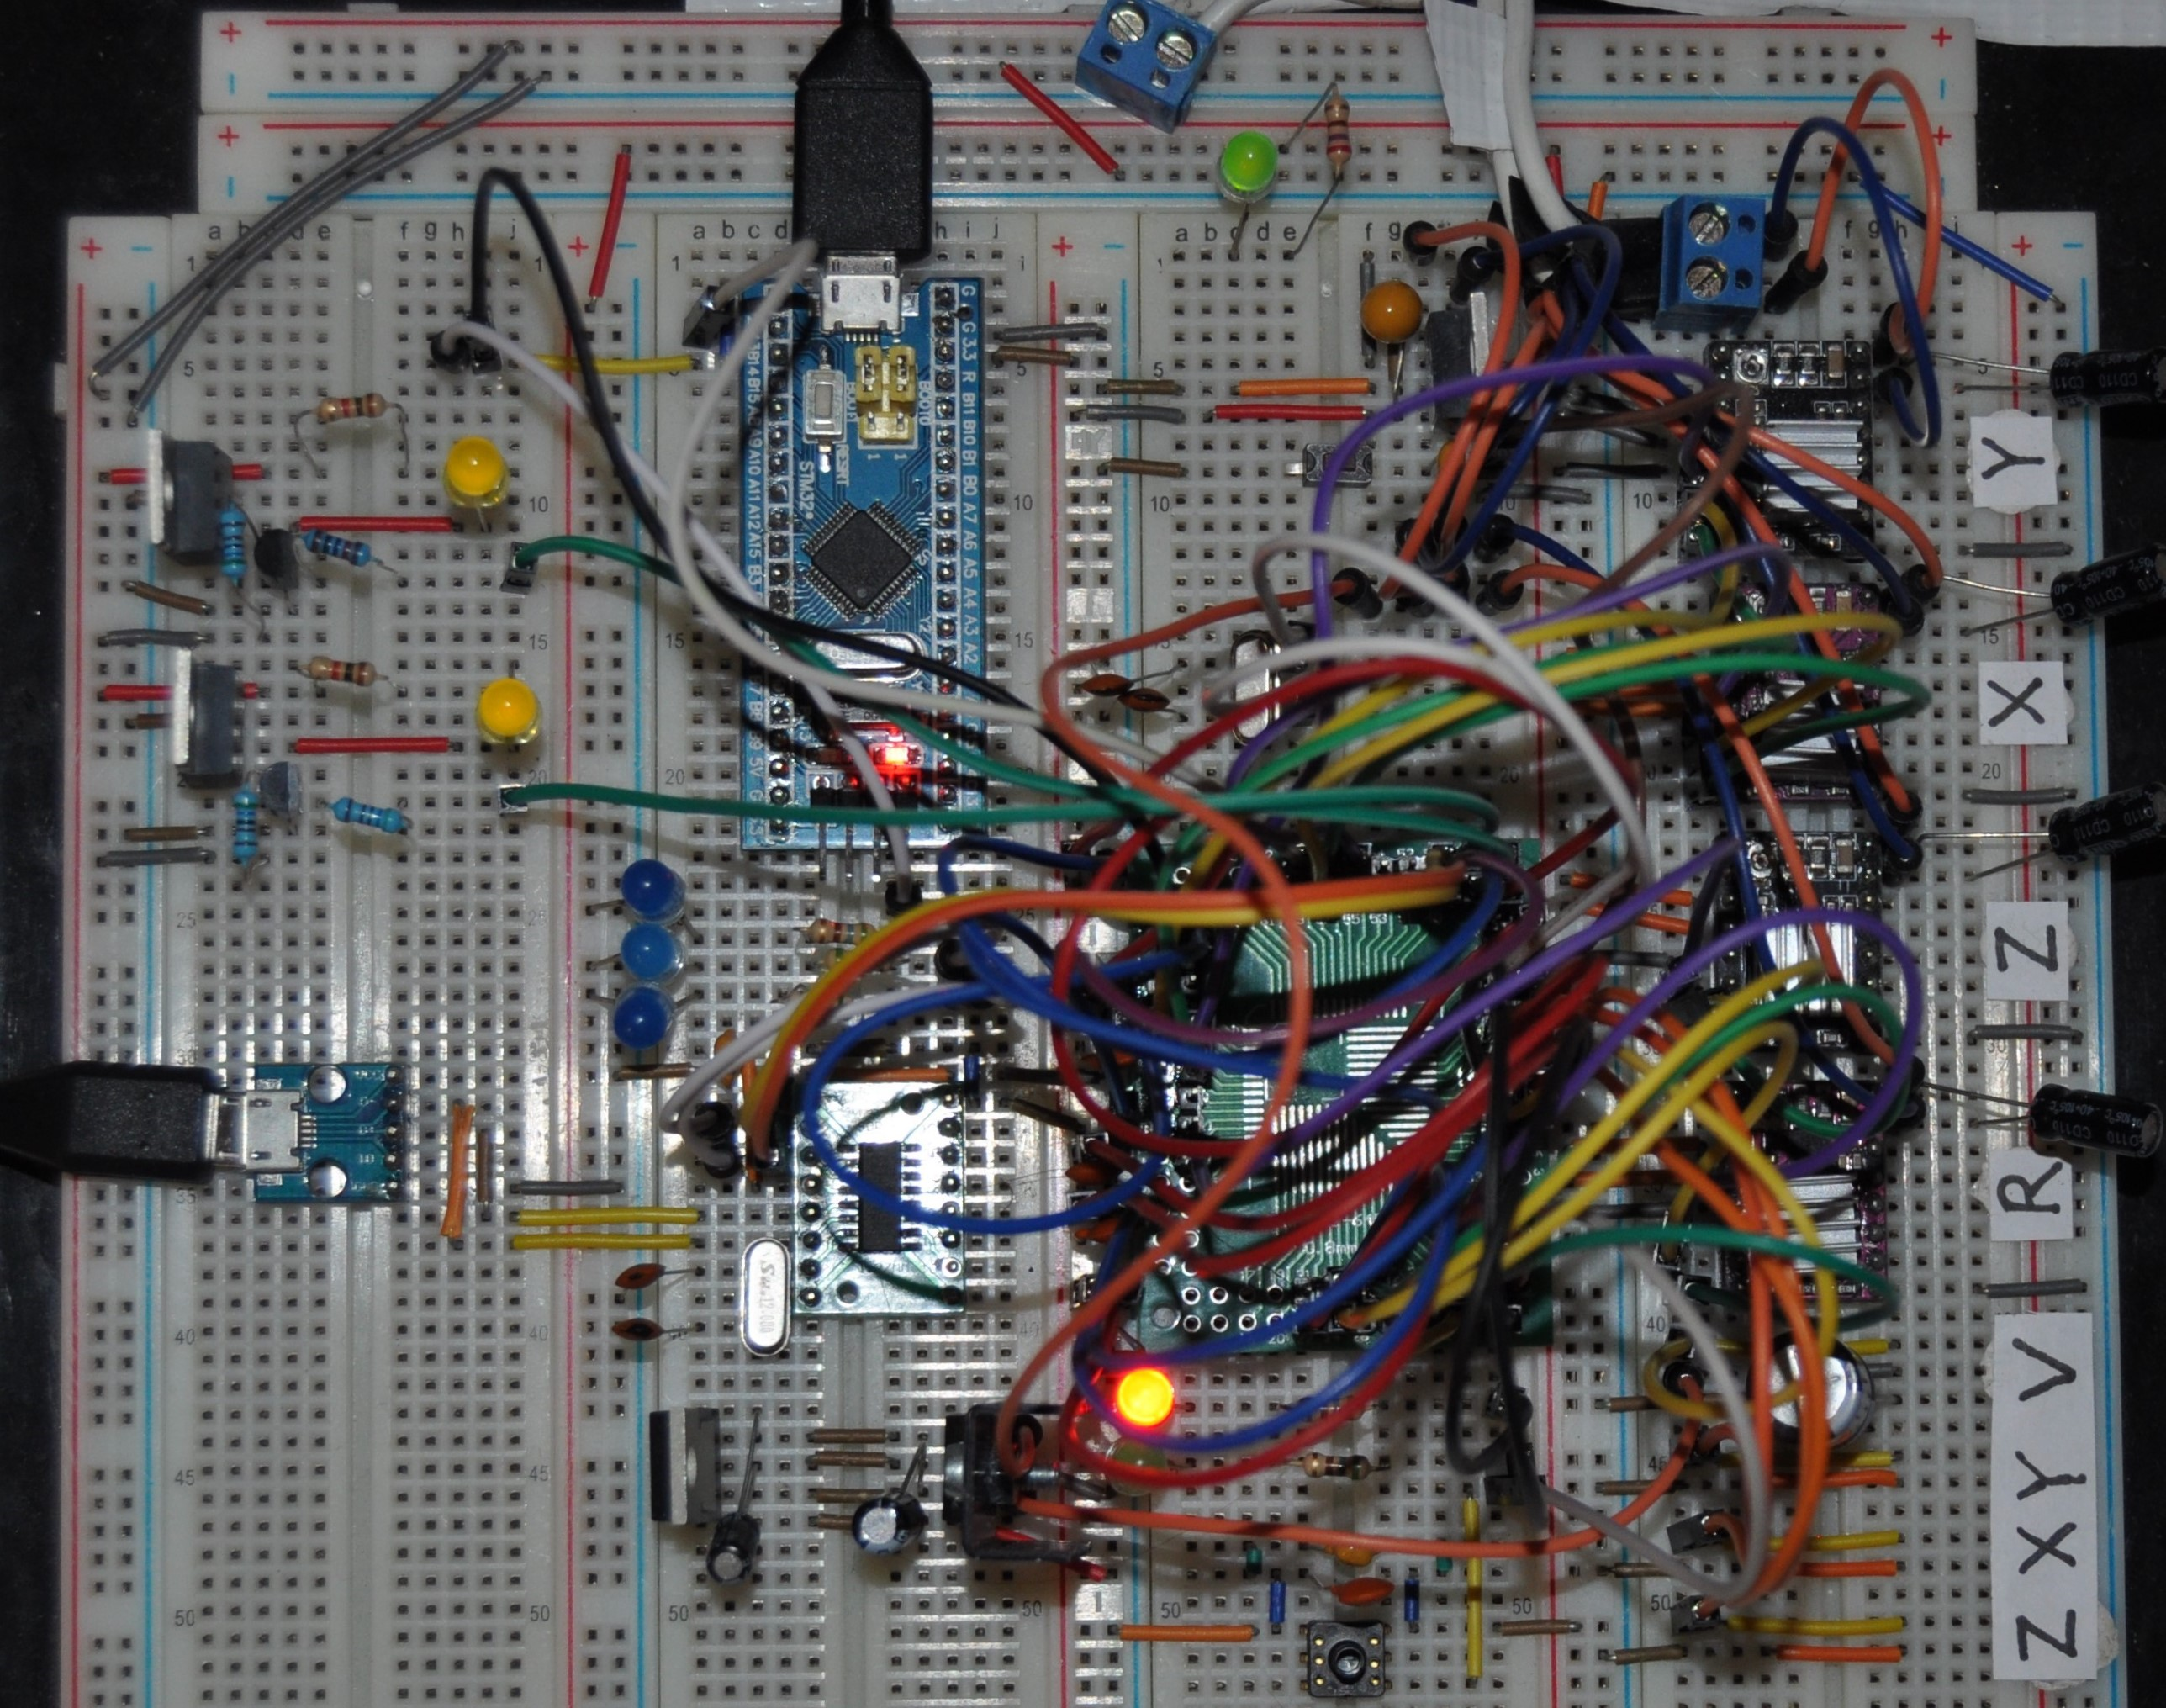
\includegraphics[width=0.6\linewidth]{figures/robotic-controller-prototype.JPG}
	\caption{Embedded robotic controller prototype.}
	\label{fig:robotic-controller-prototype}
\end{figure}

After the prototype controller was confirmed to be functioning correctly, the PCB design process was initiated. The PCB design was developed using the KiCAD schematic capture and PCB design software. The design process consisted of two steps. The first step involved the development of the electrical design in which all the electrical component pins were assigned to electrical nodes. In other words, the component connections were defined in this step. This was followed by the PCB component layout and trace routing step. In order to determine the width of the power supply trace used on the PCB, the maximum current that could flow on that trace needed to be determined based on the current ratings of the constituent components. The maximum current ratings of each of the components are listed below:

\begin{compactitem}
	\item 42BYGHW920L21B2 - 2.2 A
	\item 42BYGHW609 stepper motor - 1.7 A
	\item 35BYGH312P1 stepper motor - 1.2 A
	\item 20BYGH406 stepper motor - 0.6 A
	\item DS3118MG servo motor - 2 A
	\item STM32L072RZT6 microcontroller - 105 mA
	\item CH340G chip - 30 mA.
\end{compactitem}

Based on the sum of these values, the initial power connection trace needed to support 5.835 A of current. A current value of 6 A was used to incorporate an engineering safety margin. Furthermore, a maximum temperature rise tolerance of $10\;^{\circ}C$ and a copper thickness of $1 \text{oz/ft}^2$ was used in the calculation of the trace width. Based on this, it was calculated that a trace width of at least 140 mil, or 3.56 mm, was required. A similar procedure was used to calculate the widths of power traces that supported fewer components. For the thickness of the PCB traces, it was noted that 2 oz outer copper weight is generally notably more expensive than 1 oz outer copper weight. Therefore, the latter was used for traces for the PCB developed in this project. 

%TODO: Insert equations used to calculate the trace widths

The D+ and D- lines for the USB portion of the USB to serial converter constitute a differential pair. As such, a number of PCB layout guidelines needed to be adhered to ensure the integrity of the differential pair signal. The following guidelines were followed for this purpose:

% https://resources.pcb.cadence.com/blog/2021-efficient-differential-pair-routing-guidelines-to-speed-up-pcb-routing
\begin{compactitem}
	\item The use of vias should be minimised. 
	\item The differential pair should be isolated from the other traces. 
	\item Differential pair traces should mirror each other as far as possible.
	\item The lengths of each trace in the differential pair must be identical even if symmetry needs be sacrificed to achieve this.
\end{compactitem}

%TODO: Possibly insert image of differential pair on PCB

In this project, vias were not used at all for the differential USB signal traces. Additionally, the trace isolation condition was satisfied by enforcing a clearance of three standard trace widths from other traces for a total clearance of 0.75mm. Similarly, for both the STM32L072RZT6 external oscillator and the CH340G external oscillator, the following guidelines were adhered to during the PCB layout process:

%Oscillator
% See https://ecsxtal.com/crystal-and-oscillator-printed-circuit-board-design-considerations
\begin{compactitem}
	\item The crystal and its supporting capacitors should be placed as close as possible to the oscillator input and output pins on the microcontroller.
	\item The trace length in the oscillator circuit should be minimised.
	\item The traces in the oscillator circuit should not cross other signal lines.
	\item Traces should not incur right angle bends.
	\item The supporting capacitors should share a ground plane.
	\item The size of loops in the oscillator circuit should be minimised.
	\item The ground node should not pass under the crystal.
	\item Power and digital signal on other layers of the board should not pass under the crystal. 
\end{compactitem}

%TODO: Possibly insert image of oscillators on PCB
In addition to the PCB design components discussed above, the PCB was designed in such a manner that all the components were placed on the top layer of the two layer PCB. The top layer was referred to as the signal layer since traces were routed on the top layer as far as possible. Only when necessary, the traces were routed onto the bottom layer to pass below other traces before being returned to the signal layer by means of vias. This routing strategy allowed a ground plane fill to be applied to the majority of the bottom plane. This improved the radio frequency (RF) characteristics of the PCB as higher frequency signal components could return much more closely to their signal path which minimised the current loop size. Furthermore, the trace routing was simplified as an electrical node on the signal plane could be grounded by simply adding a via to the ground plane. The PCB layout with the routing complete is shown in Figure \ref{fig:pcb-routing} while the physical realisation of this design after manufacturing is shown in Figure \ref{fig:empty-robotic-controller}. A 3D model was created using KiCAD's rendering functionality to identify any logistical issues that could arise during the assembly process due to the 3D form factor of the components. This model is shown in Figure \ref{fig:robotic-controller-model}. The final manufactured PCB after assembly is shown in Figure \ref{fig:assembled-robotic-controller} without the motor drivers inserted.

\begin{figure}[!ht]
	\centering
	\begin{subfigure}{.5\textwidth}
		\centering
		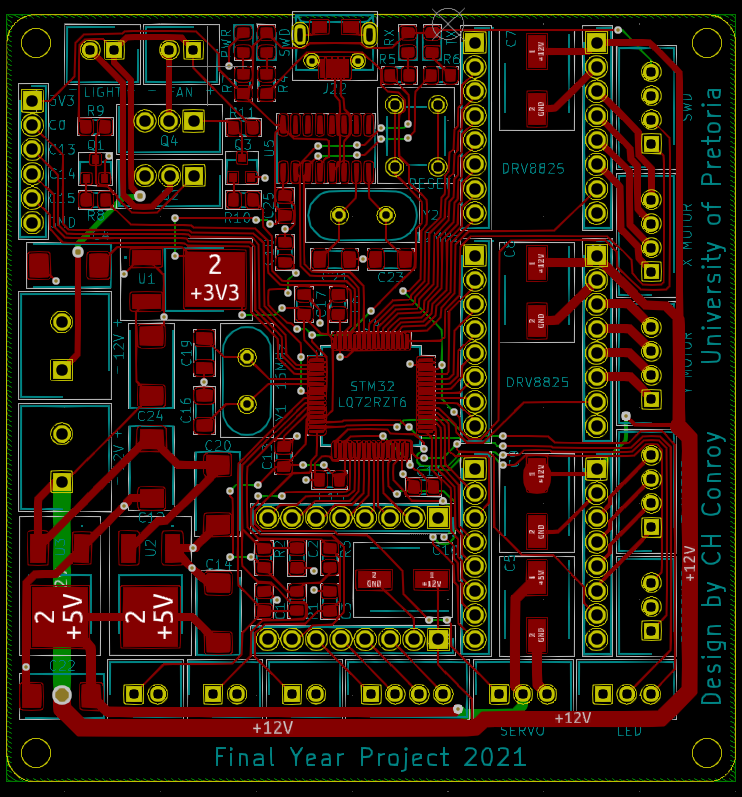
\includegraphics[width=1\linewidth]{figures/pcb-routing.png}
		\caption{Embedded controller PCB routing}
		\label{fig:pcb-routing}
	\end{subfigure}%
	\begin{subfigure}{.5\textwidth}
		\centering
		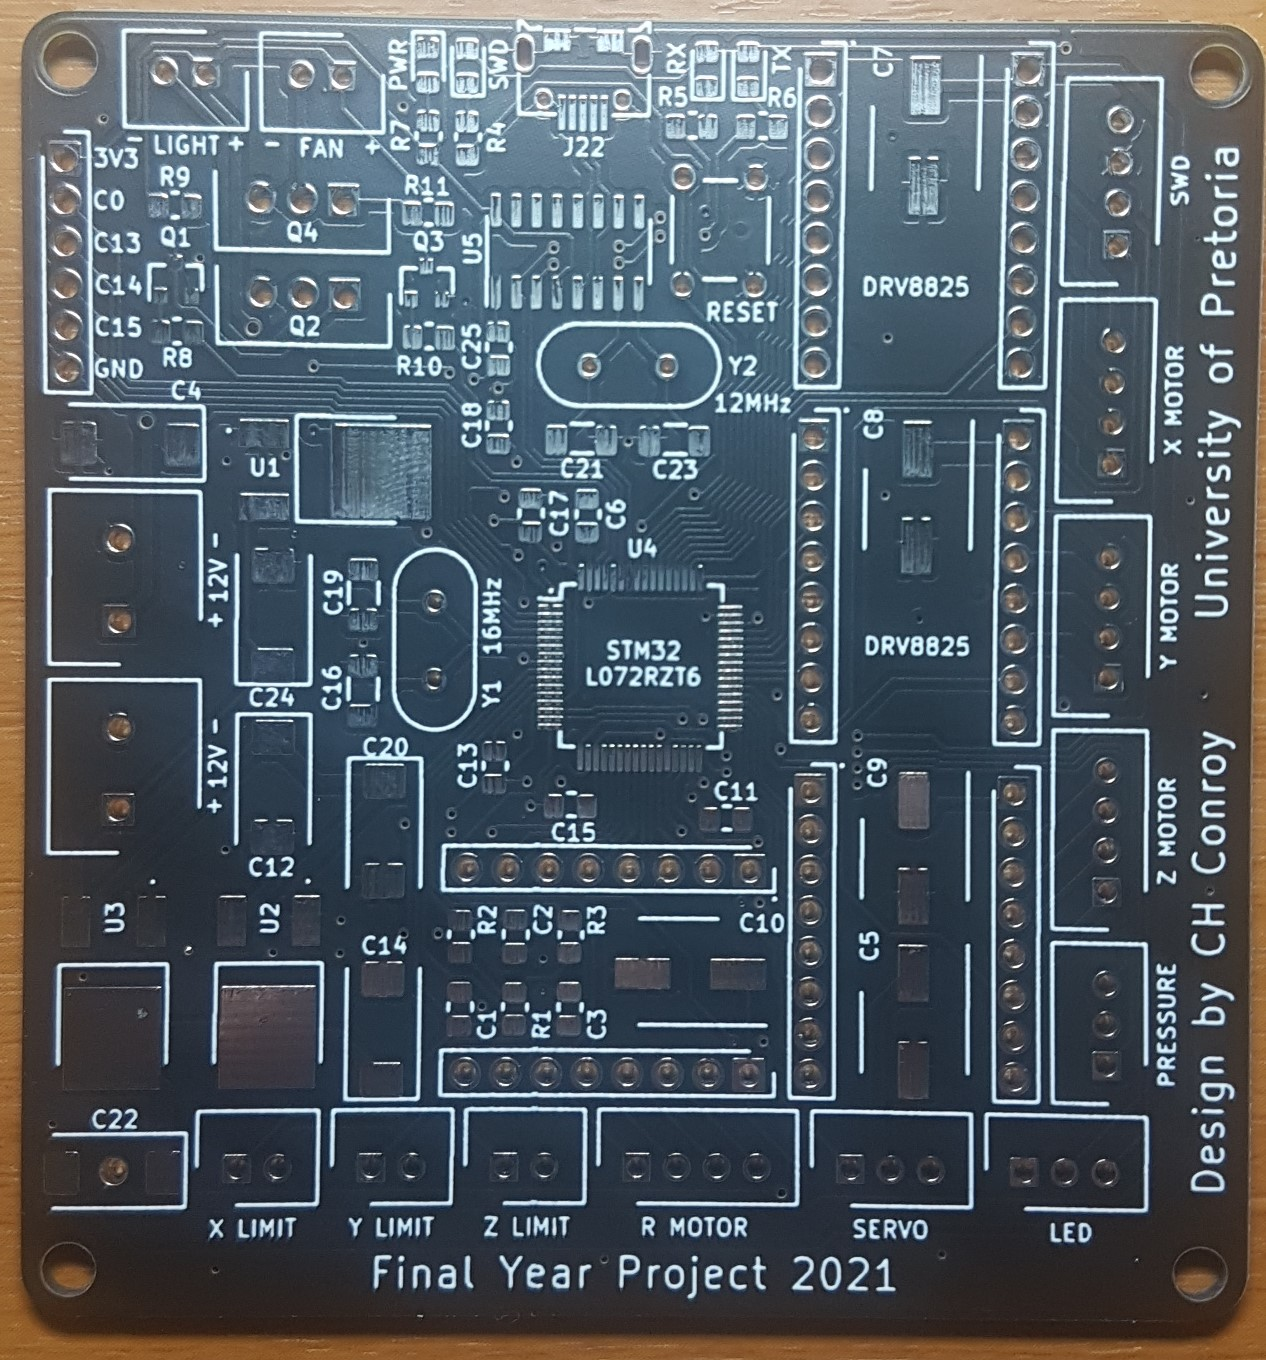
\includegraphics[width=1\linewidth]{figures/pcb-board.jpg}
		\caption{Manufactured controller PCB}
		\label{fig:empty-robotic-controller}
	\end{subfigure}%
	\caption{Design of the PCB board component and trace layout before and after manufacturing.}
	\label{fig:pcb-design-process}
\end{figure}

\begin{figure}[!ht]
	\centering
	\begin{subfigure}{.5\textwidth}
		\centering
		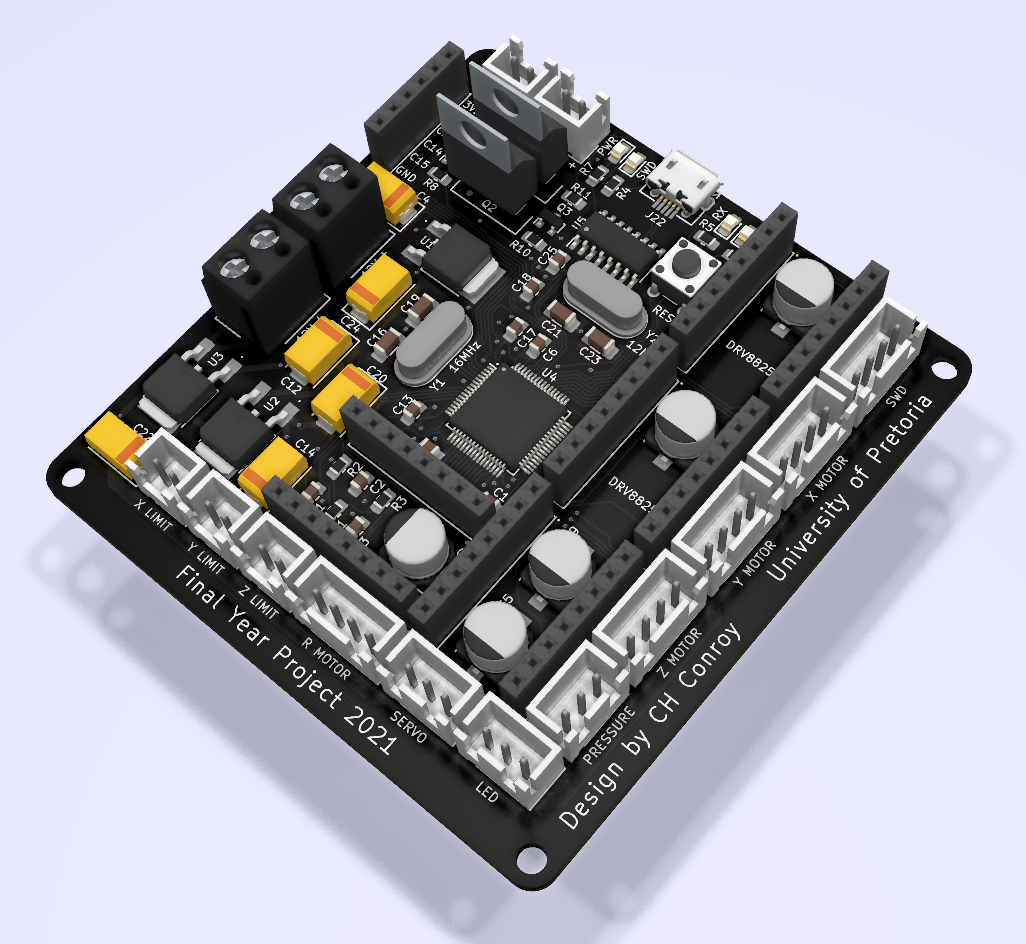
\includegraphics[width=1\linewidth]{figures/robotic-controller-model.png}
		\caption{Embedded controller PCB 3D model}
	\label{fig:robotic-controller-model}
	\end{subfigure}%
	\begin{subfigure}{.5\textwidth}
		\centering
		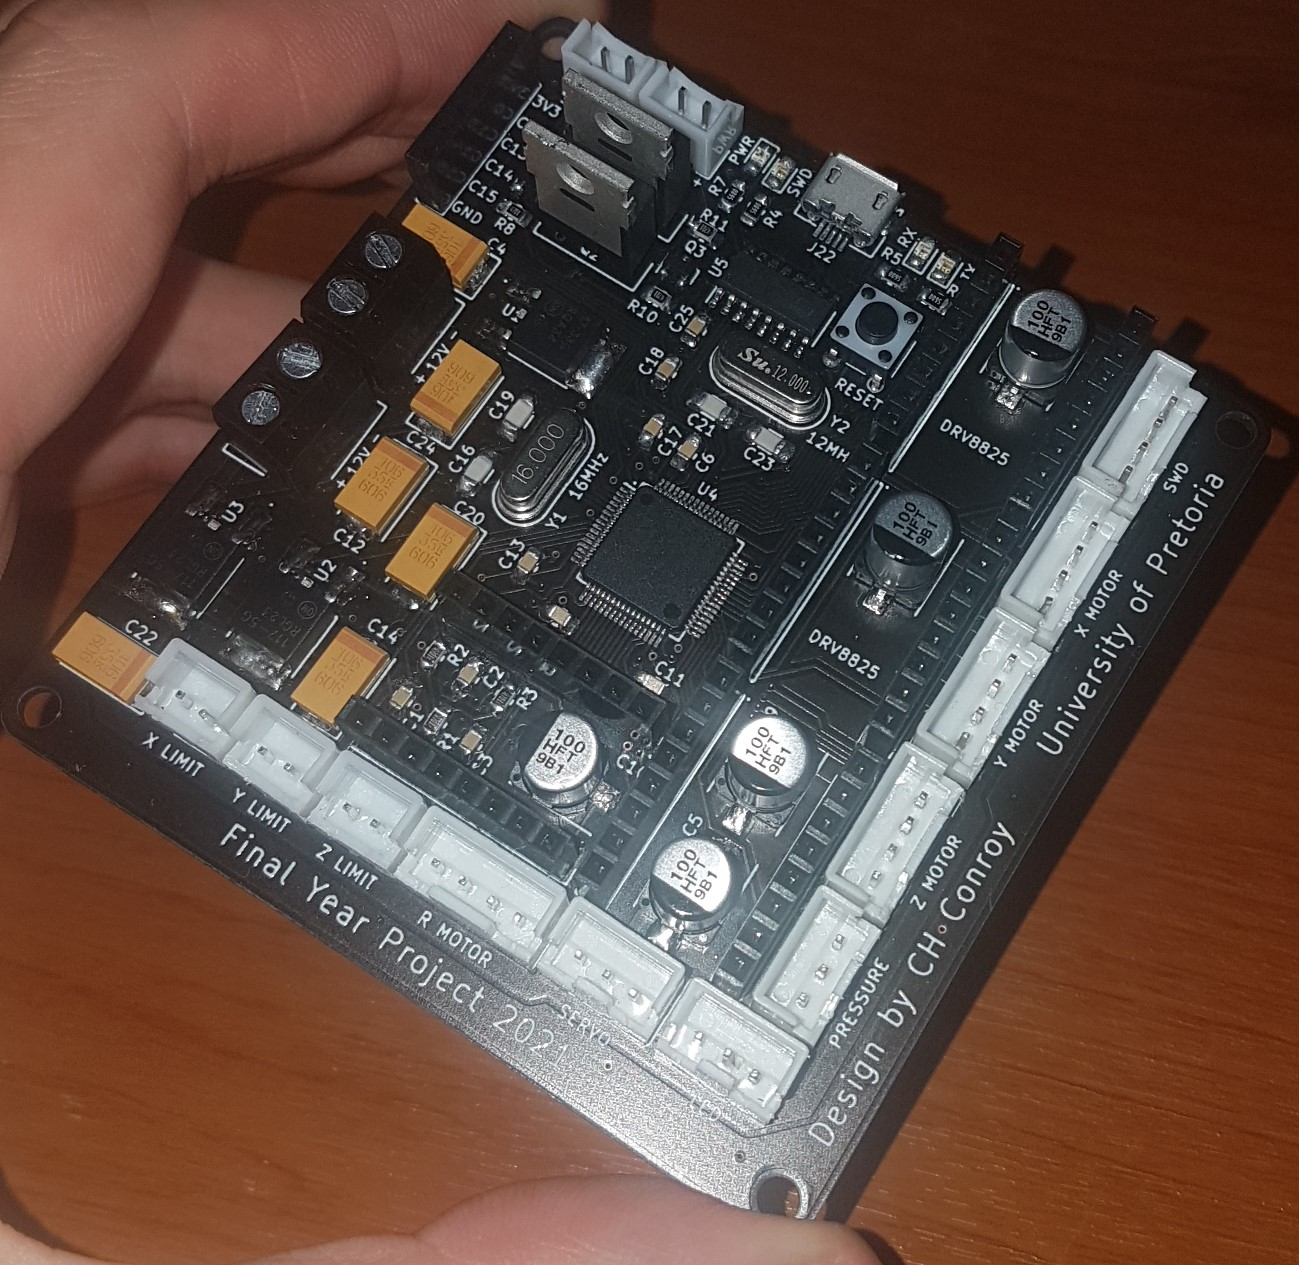
\includegraphics[width=1\linewidth]{figures/final-pcb.jpg}
		\caption{Assembled controller PCB}
	\label{fig:assembled-robotic-controller}
	\end{subfigure}%
	\caption{Final PCB after all components have been assembled.}
	\label{fig:pcb-assembly}
\end{figure}

%The components required to assemble the board were acquired prior to the delivery of the PCB board. Due to the close proximity of the components, the components were required to be strategically soldered in order to prevent any obstructions that prevented subsequent components from being soldered in their intended location. Due to the fine pitch (0.5mm) nature of the STM32L072RZT6 microcontroller package, a drag soldering technique was used in conjunction with a significant amount of solder flux to successfully solder the component. The board was cleaned using IPA alcohol throughout the soldering process. The assembled PCB board is shown in Figure \ref{fig:assembled-robotic-controller}.

%TODO: Add images of other PCBs

\subsubsection{Firmware}

\ldots

\subsubsection{Motor Control} \label{sec:Motor Control}

The DS3118MG servo motor used as the actuation driver for the vacuum generation mechanism and has a angular rotation range of $180\degree$. The medium of control for the servo motor is a PWM signal that has two degrees of freedom which motor responds to. Firstly, the period of the PWM signal determines the fraction of the angular rotation range available to the servo motor. The input period can be set from 3 ms to 20 ms (333 Hz to 50 Hz) where a period of 20 ms corresponds to the full range of rotation for the servo. Since the vacuum generation mechanism was designed on the assumption that the servo operates with $180\degree$ of rotational motion, 20 ms was chosen as the PWM period.

The second degree of freedom in control of the servo offered by the PWM signal exists in the high-time of the pulse, or pulse width. The position of the servo is altered by changing this parameter between 500$\mu s$ and 2500$\mu s$ where the bounds of this range correspond to the 0$\degree$ and 180$\degree$ servo motor positions\footnote{This assumes the PWM period is set to 20 ms.}. The release, idle and actuate positions of the vacuum generation mechanism were selected by setting the PWM pulse width to either 2400$\mu s$, 2100 $\mu s$ or 1500 $\mu s$ respectively.

%The first step in configuring PWM requires the configuration of the counter clock speed. A counter clock speed of $1\;MHz$ is desired given that the system clock frequency is $f_{CK}=32\;MHz$. These two quantities are related by the timer prescalar PSC[15:0] as
%
%\begin{align}
%	\text{CK\_CNT}=\frac{f_{CK}}{\text{PSC[15:0]}}.
%	\label{pwm-counter-clock}
%\end{align}

%Using Equation \ref{pwm-counter-clock}, the required prescalar value is calculated as 31. The DS3118MG servo motor requires a PWM period of $20\;ms$ to make use of its full rotational range of $180^{\circ}$. Given that the counter has a clock frequency of $1\;MHz$, a value of 19 999 (where 1 is subtracted since the counter counts the rollover time-step) is required as the counter reload trigger value.

As mentioned in Section \ref{sec:Circuit Design}, the DRV8825 drivers were selected to provide an interface to the microcontroller to control the stepper motors. This interface includes the \textit{STEP} control input, which moves the motor one step\footnote{The size of the step the motor takes is dependent on the microstepping mode configuration.}, as well as the \textit{DIR} control input which indicates the rotational direction in which the step is taken. The first design consideration in the control of the stepper motors is the step resolution, or microstepping mode, employed. The microstepping mode selection control inputs $M0$, $M1$ and $M2$ were connected to the microcontroller as part of the circuit design which allowed the microstepping mode to be selected in software. In general, increasing the step resolution improves the smoothness of the stepper motor rotation but also increases the pulse rate required to move the motor at the same speed. This is turn increases the computational load on the microcontroller.

The DRV8825 supports a maximum of 1/32 microstepping.\footnote{For each step in 1/32 microstepping mode, the motor rotates 1/32 of the full step angle.} Since this project has specifications relating the the accuracy of the system but not the speed of the system, the maximum microstepping mode was selected to reduce vibrations as far as possible. It was noted that increasing the microstepping resolution did not correspond to an increase in position resolution. This is due to the fact that there is an exponential reduction in holding torque in microstep positions as the microstepping resolution increases. For this reason, the motor control firmware was designed such that the stepper motors only make use of microstep positions during the movement phase to reduce vibration and only rest in full step positions.

The simplest form of control for the stepper motors is constant speed control where the rate at which pulses are sent to the motor is always constant. This was the control initially implemented. However, when the pulses are started or stopped, a near instantaneous change in velocity occurred which resulted in a peak in acceleration that induced a mechanical jolt in the \textit{Robotic System}. This limited the maximum motor speed that could be used to ensure the mechanical jolt generated was minimal. To overcome this issue, a linear acceleration profile was implemented for each stepper motor. This was achieved by altering the period of the underlying microcontroller timer peripheral for each stepper motor.

\subsubsection{Serial Communication} \label{sec:Serial Communication}

A communication protocol needs to be developed between the robotic controller and the PC running the GUI software. The PC needs to be able to issue the following commands to the robotic controller:

\begin{compactitem}
	\item Calibrate axes - The robot must home its motor to find the zero position on each axis as indicated when each limit switch is triggered. The robot must also place the rotational motor into sleep mode briefly to allow any rotational tension on the vacuum tube to be released. Following this the rotational motor must be removed from sleep mode and its current angular position reset as the zero angular position. 
	\item Go to position - The robot must move to the specified position in 3D Cartesian space as well as the specified z-axis angular position.
	\item Actuate vacuum mechanism - Set the actuation of the servo motor controlling the vacuum mechanism
	\item Report pressure in vacuum system
\end{compactitem}

For the serial communication component, a word length of 8 bits was selected with no parity bit and 1 stop bit as this the most common structure used and there was no reason to choose an altered structure. A baud rate of 115200 bits/s was also selected with the maximum oversampling rate of 16 samples chosen to minimise the effective noise during data reception. The value of USARTDIV in the \textit{USART\_BRR} register of the STM32L072RZT6 is used to define the baud rate. Different equations are used to compute the baud rate based on the oversampling frequency used. For an oversampling rate of 16, the baud equation is

\begin{equation}
	\text{Baud Rate}=\frac{f_{CK}}{\textit{USARTDIV}},
\end{equation}

where $f_{CK}$ is the system clock frequency. Given that $f_{CK}=32MHz$, the value of \textit{USARTDIV} is calculated as 

\begin{align}
	\text{USARTDIV}&=\frac{f_{CK}}{\text{Baud Rate}},\\
	&=\frac{32\times10^6}{115200},\\
	&=277.78\approx278.
\end{align} 

Since USARTDIV must be an integer value, a quantisation error is introduced when $f_{CK}$ is not divisible by
the baud rate. In order for the USART receiver to function correctly when operating in asynchronous mode, the total deviation of the clock system must be within the USART receiver's tolerances. The actual baud rate achieved using the quantised USARTDIV value is 

\begin{align}
	\text{Actual Baud Rate}&=\frac{f_{CK}}{\text{USARTDIV}},\\
	&=\frac{32\times10^6}{278},\\
	&=115107.91\;\text{bits/s}.
\end{align}

The baud rate error can then be calculated as

\begin{align}
	\text{\% Error}&=\frac{\text{Actual Baud Rate - Desired Baud Rate}}{\text{Desired Baud Rate}} \times 100,\\
	&=\frac{115107.91-115200}{15200} \times 100,\\
	&=-0.08\;\text{\%}.
\end{align}

The datasheet specifies an error tolerance of $3\%$ for the USART receiver with the given configuration. Therefore, the error is acceptable and has sufficient margin to account for other error sources such as transmitter clock deviation, local oscillator deviation and errors introduced by the transmission line.

\begin{table}[H]
	\renewcommand{\arraystretch}{1.3}
	\centering
	\begin{tabular}{|>{\raggedright}m{1.5cm}|>{\raggedright}m{3cm}|>{\raggedright\arraybackslash}m{10cm}|}
		\hline
		\textbf{} & \textbf{} & \textbf{} \\
		\hline
		\multicolumn{3}{|l|}{\textbf{}} \\
		\hline
		 & & \\
		\hline
	\end{tabular}
	\caption{\label{tab:packet-format}Packet format.}
\end{table}

\begin{table}[H]
	\renewcommand{\arraystretch}{1.3}
	\centering
	\begin{tabular}{|>{\raggedright}m{1.5cm}|>{\raggedright}m{3cm}|>{\raggedright\arraybackslash}m{10cm}|}
		\hline
		\textbf{Control Byte} & \textbf{Command} & \textbf{Description} \\
		\hline
		\multicolumn{3}{|l|}{\textbf{\textit{PC System} to \textit{Robotic System}}} \\
		\hline
		0x1 & Wake & \\
		\hline
		0x2 & Calibrate & \\
		\hline
		0x3 & Set target position & \\
		\hline
		0x4 & Actuate vacuum mechanism & \\
		\hline
		0x5 & Delay & \\
		\hline
		0x6 & Request pressure update & \\
		\hline
		\multicolumn{3}{|l|}{\textbf{\textit{Robotic System} to \textit{PC System}}} \\
		\hline
		0x1 & Command complete & \\
		\hline
		0x6 & Pressure update & \\
		\hline
	\end{tabular}
	\caption{\label{tab:serial-communication-protocol}Serial communication protocol utilised between the \textit{PC System} and the \textit{Robotic System}.}
\end{table}

\subsection{Shape Definition Interface} \label{sec:Shape Definition Interface}

\subsubsection{Background}

The second system specification for this project requires the development of a PC-based GUI software component that allows the user to define 3D shapes to be constructed by the robot using the small construction cubes. Furthermore, this specification also indicates that this software component must make use of graphical primitives to generate a 3D render of the shape as part of this process. To this extent, the OpenGL specification was selected as the basis for the 3D rendering component. DirectX was considered as an alternative to OpenGL. However, DirectX is only supported for the Windows operating system and XBox while OpenGL is cross-platform. The C++ QT framework used as the basis for the PC-based software component is inherently cross-platform and also offers better support for OpenGL integration which justified its selection for use in this project. It is noted that OpenGL is only a specification for a graphics API and not an implementation in itself. This API is usually implemented by the graphics card manufacturers. Furthermore, it is noted that OpenGL can be considered to be a state machine which is referred to as the graphical context. The behaviour of various OpenGL instructions depends on the state of the OpenGL context.

The approach to developing the \textit{Shape Definition} component was split into two phases. The first phase involved the prototype development of the component in an environment isolated from the QT environment. The Graphics Library Framework (GLFW) was used to provide a simple window to render and manage the OpenGL context in as well as to provide basic mechanisms of interaction with this window through computer peripherals. Secondly, as OpenGL is just a specification, there are a number of versions of drivers that implement this specification. However, the location of these drivers is usually unknown at the point of compilation and, as a result, their locations need to be fetched upon execution of the OpenGL dependent program. In order to overcome this issue, the OpenGL loading library, GLAD, was used to fetch the location of such drivers and makes them available for use in the OpenGL prototype. The second phase of the \textit{Shape Definition} component development process involved the integration of the OpenGL prototype with the QT-based PC software component. Specifically, the \textit{QOpenGLWidget} QT class was used to facilitate this, which is essentially an OpenGL wrapper class that allows native OpenGL API calls and offers functionality similar to both GLFW and GLAD.

The foundation of rendering using OpenGL is centred around the use of vertices. Specifically, a number of vertices are defined as the starting point for various objects to be rendered in 3D. These vertices are assembled into primitive shapes such as lines, triangles, quadrilaterals and other polygons depending on the OpenGL context. Triangles were used as the primitive shape created from vertices in this project since it is straightforward to define cubes through the use of triangles and most OpenGL hardware supports render acceleration for triangles. Surfaces are created by generating a number of these shapes adjacent to each other with varying sizes and orientations. These vertices and shapes encounter a number of processes and transformations when being converted from a description in 3D space to a collection of pixels on a 2D computer screen. There are approximately six such steps in this process which are known as the six stages of the graphics pipeline which is shown in Figure \ref{fig:graphics-pipeline}.

% TODO: Replace graphics pipeline image

\begin{figure}[H]
	\centering
	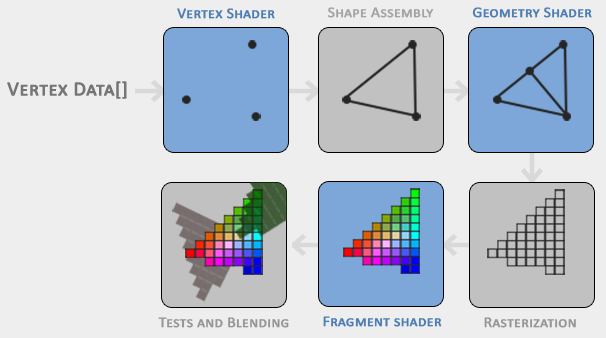
\includegraphics[width=0.7\linewidth]{figures/graphics-pipeline.PNG}
	\caption{Six stages of the graphics pipeline.}
	\label{fig:graphics-pipeline}
\end{figure}

Two of the stages shown in Figure \ref{fig:graphics-pipeline} require an implementation to be defined when using OpenGL, namely the vertex shader and the fragment shader. These shaders were written using the  OpenGL Shading Language (GLSL)\footnote{GLSL is a high-level language with C-style syntax that executes on graphics hardware and allows modification of the graphics pipeline.}. In order to define the positions and orientations of the various objects to be rendered as well as how they are transformed to 2D space on the screen, a number of coordinate systems and transformation matrices are required. These are shown in Figure \ref{fig:transformation-matrices} below.

% TODO: Replace transformation matrix image with custom renders of cube in each of these states

\begin{figure}[!ht]
	\centering
	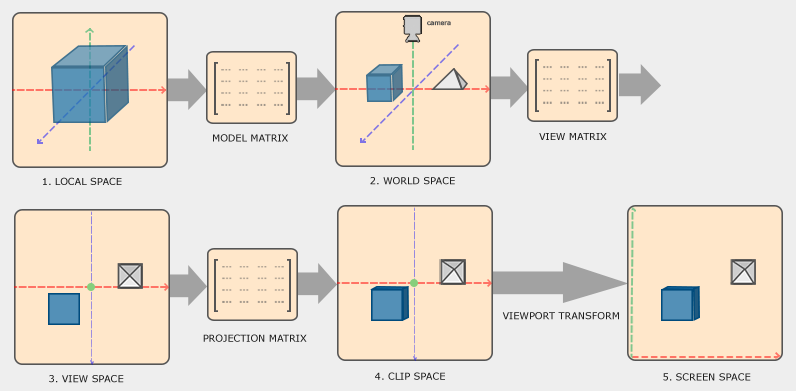
\includegraphics[width=1\linewidth]{figures/transformation-matrices.PNG}
	\caption{Transformation matrices involved in mapping the vertices from local space to screen space.}
	\label{fig:transformation-matrices}
\end{figure}

The object is described in the local frame \textit{l} with the origin of the frame of reference usually located somewhere on or within the object. The world frame \textit{w} is the space  that relates the position, orientation and scale of all the objects to be rendered together. The matrix that maps the local frame to the world frame is known as the model matrix, denoted here by $\matr{M}^{wl}$. Similarly, the view of the world, usually thought of as a camera, has its own coordinate system called view space \textit{v}. The world space is mapped to this view space by means of the view matrix $\matr{M}^{vw}$. This defines the point of view the world is seen from. Lastly, it is noted that the coordinates that are mapped to the screen need to be normalized device coordinates (NDC) where all vertex values of the coordinate axes are between 0 and 1. Any vertex outside of this space will not be projected onto the screen. As such, this space is called clip space \textit{c} and the projection matrix $\matr{M}^{cv}$ is used to map from view space to clip space. The projection matrix can be used to define the nature of this clip space and as such can be used to control the projection perspective. 

Lastly, the viewport transform is performed to convert the 3D coordinates to 2D coordinates. The former three transforms, namely the model, view and projection matrices, are the transforms that were manipulated to transform the vertices accordingly. Each of these matrices consist of a translation, rotation and scale sub-component of which the order of operations is important to ensure the correct transform result.

% TODO: Possibly add description of OpenGL coordinate system

\subsubsection{3D Shape Render}

The 3D shape to be rendered was approached by first considering how each individual constituent cube within the shape should be rendered. Since triangles were selected as the graphical shape primitive, the cube was formed by defining the six cube faces using two triangles per face. Each triangle was defined by specifying the location of each vertex in the local coordinate system for a total of 36 vertices to define the entire cube as shown in Figure \ref{fig:cube-triangles-render}. Furthermore, in order to map a texture to the cube face, each triangle vertex was associated with an NDC in the texture image file shown in Figure \ref{fig:cube-texture} such that the entire texture image was mapped to each cube face. Let $\vect{p}^l_i\in\mathbb{R}^3$ denote the position of the \textit{i}th vertex in the local coordinate system and let $\vect{t}_i\in\mathbb{R}^2$ denote the NDC in the texture image associated with $\vect{p}^l_i$. In order to capture the structure and texture of the cube to be rendered, a vertex information array was defined as

\begin{equation}
	\textit{vertices}=[\vect{p}^l_0, \vect{t}_0, \vect{p}^l_1, \vect{t}_1,...,\vect{p}^l_{35}, \vect{t}_{35}].
	\label{eqn:vertex-array}
\end{equation}

Vertex attribute pointers were created to indicate the location of the position and texture coordinates within the \textit{vertices} array in Equation \ref{eqn:vertex-array} for the OpenGL context. To render the cube using this vertex information the \textit{vertices} array was bound to the current OpenGL context using various calls to the OpenGL API. However, this resulted in only the front 2D cube face being rendered on the screen. In order for multiple cubes to be rendered from different perspectives, the model, view and projection matrices need to be derived and utilised. The model matrix is constructed by noting that a given cube is mapped from local space to world space through scaling, rotation and translation operations. Let the matrices $\matr{S}\in\mathbb{R}^{4\times4}$, $\matr{R}\in\mathbb{R}^{4\times4}$ and $\matr{T}\in\mathbb{R}^{4\times4}$ represent these operations respectively in homogeneous coordinates. Furthermore, let $\vect{v}^l_i\in\mathbb{R}^4$ denote the position of the \textit{i}th vertex in homogeneous coordinates in the local frame. Since each cube only needed to be rotated about the y-axis, $\matr{R}$ can be simplified for only this rotation as $\matr{R}_y$. Additionally, Euler angles were chosen to parameterise the cube's orientation since Gimbal lock is not possible with the rotation restricted as such. Based on this, the model matrix is calculated as

\begin{align}
	\matr{M}^{wl}&=\matr{T}\matr{R_y}\matr{S},\\
	&=
	\begin{bmatrix}
		1 & 0 & 0 & T_x\\
		0 & 1 & 0 & T_y\\
		0 & 0 & 1 & T_z\\
		0 & 0 & 0 & 1
	\end{bmatrix}
	\begin{bmatrix}
		\cos\theta & 0 & \sin\theta & 0\\
		0 & 1 & 0 & 0\\
		-\sin\theta & 0 & \cos\theta & 0\\
		0 & 0 & 0 & 1
	\end{bmatrix}
	\begin{bmatrix}
		S_x & 0 & 0 & 0\\
		0 & S_y & 0 & 0\\
		0 & 0 & S_z & 0\\
		0 & 0 & 0 & 1
	\end{bmatrix}
\end{align}

where $(T_x, T_y, T_z)$ is the translation vector, $(S_x, S_y, S_z)$ is the scaling vector and $\theta$ is the angle of rotation of the cube about the y-axis. The \textit{vertices} vector was defined in such a manner that the cube has a side length of 1 unit in the local coordinate system. Since the end-effector in the \textit{Robotic System} can only be positioned at a number of discrete \textit{step} positions, it was chosen to use \textit{steps} as the measurement unit for the world space coordinate system in the \textit{Shape Definition} component. A physical construction cube has a side length of 64 \textit{steps}. Therefore, a scaling factor of 64 \textit{steps} was used for all axes to form $\matr{M}^{wl}$. The translation vector values were obtained from the position state of the centre of a given cube in \textit{steps}. Furthermore, the translation vector element $T_y$ was offset by 32 \textit{steps} to ensure no part of the cube exists below the plane $z=0$ in the world frame.

The cubes in the world space are mapped to the view space next using the view matrix. The result of this transformation gives the impression that the world space is rendered from the perspective of a camera. This idea was used as the basis to form the view matrix\footnote{In this case, the view matrix is also frequently referred to as the \textit{LookAt} matrix.} using the camera's position $\vect{p}^w_c\in\mathbb{R}^3$, the camera's focal point $\vect{p}^w_f\in\mathbb{R}^3$ and the camera's up direction vector $\hat{\vect{u}}^w_u\in\mathbb{R}^3$, all with respect to the world frame. The camera direction\footnote{Unintuitively, the camera direction vector points in direction opposite to the direction the camera is facing.} vector $\hat{\vect{u}}^w_z\in\mathbb{R}^3$ (i.e. camera's positive z-axis) is calculated as

\begin{align}
	\vect{u}^w_z&=\vect{p}^w_c-\vect{p}^w_f,\\
	\hat{\vect{u}}^w_z&=\frac{\vect{u}^w_z}{||\vect{u}^w_z||}.
	\label{eqn:opengl-camera-z}
\end{align}

With the direction of the camera known, the camera's right vector $\hat{\vect{u}}^w_x\in\mathbb{R}^3$ (i.e. camera's positive x-axis) in the world frame is calculated as

\begin{align}
	\vect{u}^w_x&=\hat{\vect{u}}^w_u\times\hat{\vect{u}}^w_d,\\
	\hat{\vect{u}}^w_x&=\frac{\vect{u}^w_x}{||\vect{u}^w_x||}.
	\label{eqn:opengl-camera-x}
\end{align}

Finally, the direction of the camera's positive y-axis $\hat{\vect{u}}^w_y\in\mathbb{R}^3$ with respect to the world frame is calculated as

\begin{equation}
	\hat{\vect{u}}^w_y=\hat{\vect{u}}^w_z\times\hat{\vect{u}}^w_x.
	\label{eqn:opengl-camera-y}
\end{equation}

The results of Equations \ref{eqn:opengl-camera-z}, \ref{eqn:opengl-camera-x} and \ref{eqn:opengl-camera-y} are used to calculate the view matrix as

\begin{equation}
	\renewcommand*{\arraystretch}{1.3}
	\matr{T}^{vw}=
	\begin{bmatrix}
		\hat{u}^w_{x,0} & \hat{u}^w_{x,1} & \hat{u}^w_{x,2} & 0 \\
		\hat{u}^w_{y,0} & \hat{u}^w_{y,1} & \hat{u}^w_{y,2} & 0 \\
		\hat{u}^w_{z,0} & \hat{u}^w_{z,1} & \hat{u}^w_{z,2} & 0 \\
		0 & 0 & 0 & 1
	\end{bmatrix}
	\begin{bmatrix}
		1 & 0 & 0 & -p^w_{c,0} \\
		0 & 1 & 0 & -p^w_{c,1} \\
		0 & 0 & 1 & -p^w_{c,2} \\
		0 & 0 & 0 & 1
	\end{bmatrix}
\end{equation}

where $\hat{u}^w_{x,i}$, $\hat{u}^w_{y,i}$, $\hat{u}^w_{z,i}$ and $p^w_{c,i}$ are the \textit{i}th elements of $\hat{\vect{u}}^w_{x}$, $\hat{\vect{u}}^w_{y}$, $\hat{\vect{u}}^w_{z}$ and $\vect{p}^w_{c}$ respectively. The final transformation that was implemented is the mapping of view space to clip space using the projection matrix. The points that are clipped are selected based on their location with respect to a frustum defined in the view frame. Points that fall within this frustum are kept and converted to NDCs while points outside of this frustum are clipped. The shape of this frustum defines the nature of the projection. Specifically, if the frustum is a rectangular prism, the resulting projection is an orthographic projection. However, if the frustum is not a uniform prism, the resulting projection is a perspective projection. The perspective projection is how the world appears to the human eye and, therefore, was selected as the projection method for this project to ease the process of comparing the 3D shape model and the constructed shape. The projection matrix is defined as

\begin{equation}
	\matr{T}^{cv}=
	\begin{bmatrix}
		\frac{n}{r} & 0 & 0 & 0 \\
		0 & \frac{n}{t} & 0 & 0 \\
		0 & 0 & \frac{-(f+n)}{f-n} & \frac{-2fn}{f-n} \\
		0 & 0 & -1 & 0
	\end{bmatrix}
\label{eqn:projection-matrix}
\end{equation}

where $n$ and $f$ are the near and far z-planes of the projection frustum respectively in the view frame. Furthermore, $r$ and $t$ are the right and top bounding x- and y-planes respectively for the near frustum z-plane. Equation \ref{eqn:projection-matrix} assumes that the frustum exhibits x and y symmetry such that the left and bottom bounding planes need not be specified. It was found to be more intuitive to parameterise the projection in terms of the frustum angle $\alpha$ and aspect ratio $\beta$ of the frustum z-planes alongside $f$ and $n$. To this end, $n/r$ and $n/t$ in Equation \ref{eqn:projection-matrix} are computed as

\begin{align}
	\frac{n}{r}&=\frac{1}{\alpha\tan(\beta/2)}\\
	\frac{n}{r}&=\frac{1}{\tan(\beta/2)}
\end{align} 

\begin{figure}[!ht]
	\centering
	\begin{subfigure}{.32\textwidth}
		\centering
		
\includegraphics[width=0.8\linewidth]{figures/cube-texture.jpg}
		\caption{Cube face texture}
		\label{fig:cube-texture}
	\end{subfigure}%
	\begin{subfigure}{.32\textwidth}
		\centering
		
\includegraphics[width=0.8\linewidth]{figures/cube-triangles-render.PNG}
		\caption{Triangle components}
		\label{fig:cube-triangles-render}
	\end{subfigure}%
	\begin{subfigure}{.32\textwidth}
		\centering
		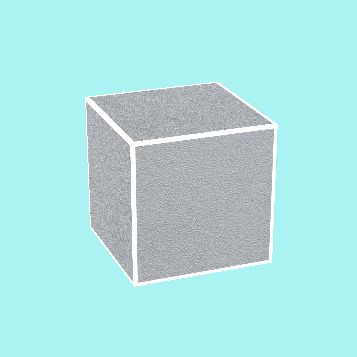
\includegraphics[width=0.8\linewidth]{figures/cube-render.PNG}
		\caption{Textured cube}
		\label{fig:cube-render}
	\end{subfigure}%
	\caption{Stages of the process to render a construction cube using OpenGL.}
	\label{fig:opengl}
\end{figure}

By defining cubes using vertex arrays and manipulating these vertices as described above, a pyramid 3D shape that the robot could build was rendered as shown in Figure \ref{fig:initial-opengl} below.

\begin{figure}[!ht]
	\centering
	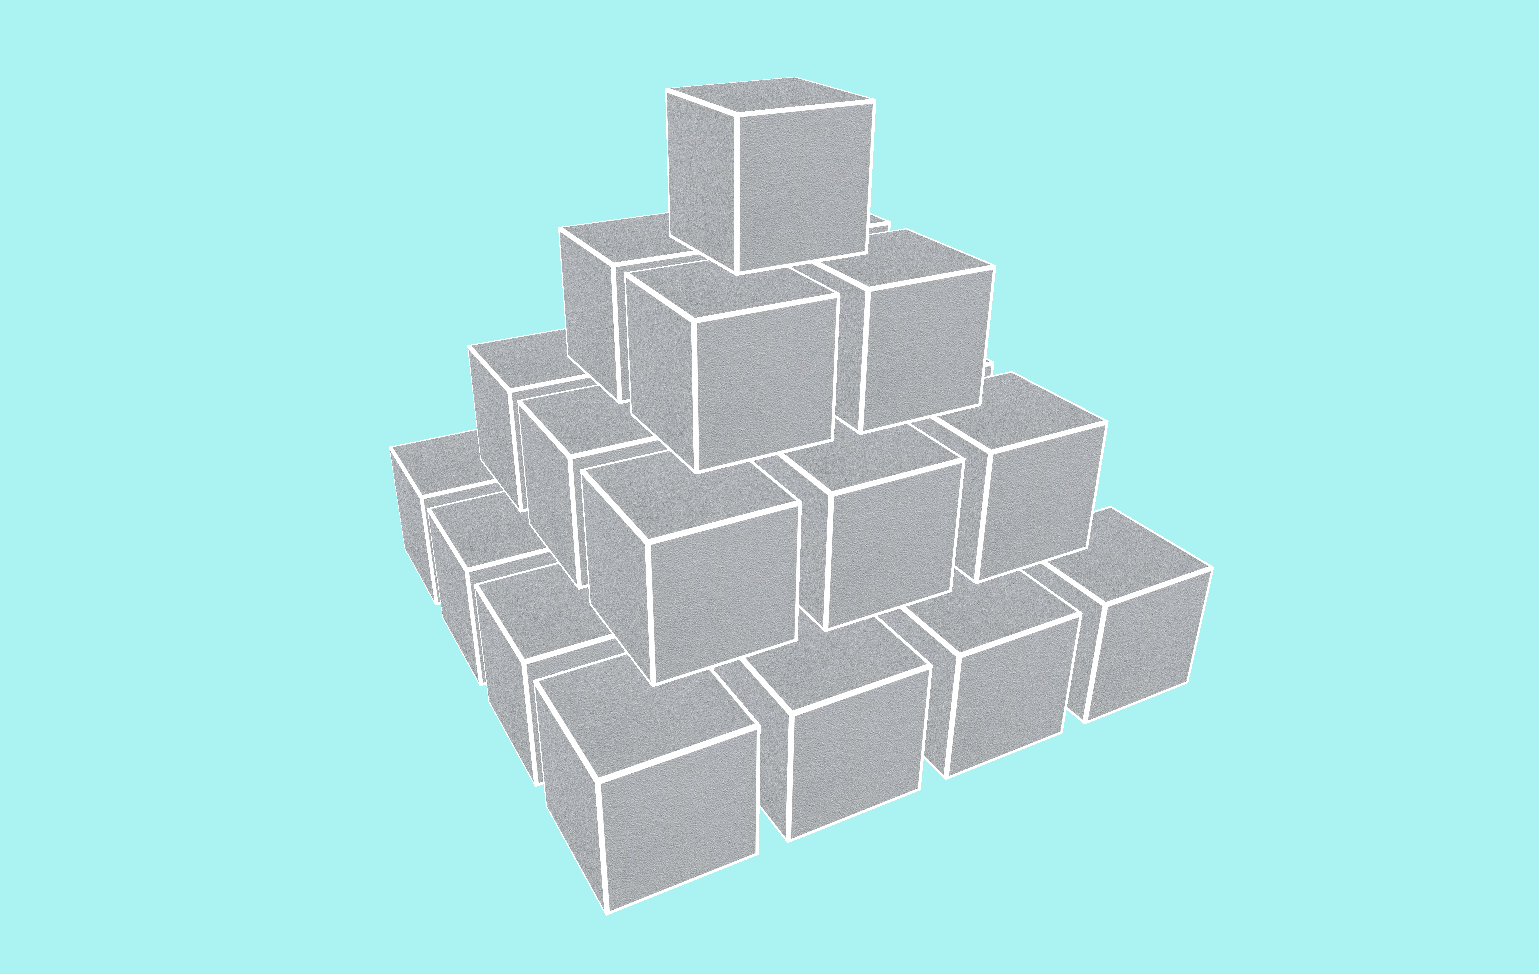
\includegraphics[width=0.8\linewidth]{figures/initial-opengl-shape.PNG}
	\caption{3D render of pyramid shape generated using OpenGL within QT framework.}
	\label{fig:initial-opengl}
\end{figure}


\subsubsection{User Control}

The desired camera behaviour was defined as follows:

\begin{compactitem}
	\item The camera frame x-axis should remain parallel to the world xz plane.
	\item The camera movement about a point should always be on the surface of a dome about that point when not translating or zooming.
	\item As the camera rotates the camera should continue to look at the same focal point.
\end{compactitem}

%\begin{compactitem}
%	\item Camera control by means of computer peripherals was implemented. The right mouse button can be used to control the rotation of the camera about a given focal point. The middle mouse button can be used to translate the camera horizontally in the world scene.
%	\item The OpenGL shape render view was integrated with the main software GUI component.
%	\item The ability for the user to insert and remove shapes from the model as well as the ability for the user to specify the position and rotation of the cube within the 3D model space.
%	\item The option to load and save model files.
%\end{compactitem}

\subsection{Computer Vision System} \label{sec:Computer Vision System}

The design of the overall system facilitates open-loop operation of the robotic subsystem when the computer vision subsystem is excluded. This means that the system is capable of arbitrary shape construction without visual feedback during the construction process, given that the initial cube positions are known. However, should a cube be dropped during this process, the system would not be capable of an intelligent response\footnote{The system would be able to detect the dropped cube condition through the pressure sensor in the vacuum system detecting the unplanned pressure decrease.}. Furthermore, any significant disturbance of the shape under construction would be undetectable by the system. The computer vision system is required, and was designed, to address these two cases. In the first case, the dropped cube should be detected and localised with respect to the robot coordinate system if it falls within the camera's field of view. Secondly, when damage to the structure is detected in the image input data, the computer vision system should signal a construction halt condition. This section begins with an overview of the cube detection approaches investigated. A description of the method used to map points detected in the image frame to the world frame follows in Section \ref{sec:3D Localisation}. These sections lay the foundation for the integrated computer vision algorithm and supporting functions discussed from Section \ref{sec:Top-Level Design} onward.

\subsubsection{Cube Feature Investigation} \label{sec:Cube Feature Investigation}

Detection of an object in a single-view image generally involves the identification of features in the image which can be compared to a template set of features for the desired object to determine its presence and location in the image. Furthermore, certain features may be used in to generate further information about the object beyond feature matching. For example, edges and corners may be used to identify planes which are combined to identify the presence of a cuboid. The OpenCV C++ library was utilised as the source of various pre-written image processing and machine vision functions required to create a prototype of the feature detection process. Specifically, a set of cube images were captured and the Canny edge detector, Harris corner detector and SIFT feature descriptor implementations were utilised to detect edges, corners and features in the cube images respectively. 

The primary challenge encountered in cube detection process was the extraction of useful feature information from individual cubes. The aluminium cubes used in this project are a singular shade of grey with an almost textureless surfaces which offers little unique information to detect the cubes. As a result, the prototype feature detection algorithms discussed above performed poorly and did not extract a sufficient number of features to uniquely detect the cubes. Specifically, in even lighting conditions, the Canny edge detector failed to identify internal edges within the outer bounding contour. Similarly, the Harris corner detector failed to consistently identify the corners of the cube while the SIFT algorithm failed to identify a sufficient number of features on the cube itself. The Hough transform parameterised for lines was also explored with limited success.  

The process of image segmentation was also explored to isolate the cubes from the background. Histogram plots showing pixel intensity distributions for each of the RGB colour channels were generated from images containing cubes with various monochrome background colours. Each of he colour channels exhibited nearly identical distributions which indicated the primary information in these images was grey-scale intensity information. The grey-scale histogram information from the images with a matte black background exhibited a peak at greater pixel intensity values corresponding with the cube pixels. Based on this, the cubes were successfully segmented in the image through through application of a binary threshold. 

In even lighting conditions, the cube faces could not be distinguished from each other with a significant degree of reliability. This presents a problem as face segmentation is necessary for cube pose estimation. However, when the dominant lighting source was placed directly above the cubes, a peak in the pixel intensity histogram was observed which corresponded to the top face of the cube. This allowed the segmentation of the top face with a great degree of reliability. If the scene is constrained such that cubes are the only objects present and the assumption is made that a cube face is always parallel to the base plane, then the segmented top cube face is sufficient information to detect a cube and uniquely determine its orientation about the z-axis. Therefore, this approach was selected as the basis of the computer vision cube detection component.

%Colour Segmentation with Overhead Lighting
%
%Although the cube was successfully segmented as shown in Figure X the following points must be made:
%
%\begin{compactitem}
%	\item The cube had relatively even lighting from several angles. This caused all the faces to have a similar grey intensity which facilitated intensity segmentation but introduced difficulties with reliable face segmentation.
%	\item By using a plain black background, colour information does not play a role in the segmentation process.
%	\item The image of the cube is relatively high resolution which may not be possible in the final project configuration.
%	\item The camera is likely to be located relatively high above the cubes in which case such low angle images of the cube are unlikely to be processed.
%\end{compactitem}
%
%To explore the possibilities for cube recognition further, the above points were investigated. Figure X shows the image of the cube captured from a high angle with a plain blue paper background and diffuse overhead lighting. The first interesting point noted from this image is the intensity of the pixels corresponding to the top face of the cube. This high intensity was present even when the position of the cube and camera were varied provided the angle was sufficiently high. The following points are made considering this observation:
%
%\begin{compactitem}
%	\item Given the constrained nature of cube recognition problem, knowledge of the top face of the cube should be sufficient to identify both the location and the pose of the cube.
%	\item Due to the light dispersion that occurs from the sand-blasted cube surface, a significant mirror effect does not occur on the cube surface despite the intensity of light reflection. This is beneficial as mirror-like surfaces introduce complications in machine vision problems.
%	\item If the lighting conditions are well-controlled, the top-face of the cube can be potentially be reliably segmented from the image. It is much simpler to extract geometric information from a segmented square face than from a given segmented view of a cube.
%\end{compactitem}
%
%Centroid Detection for Multiple Cubes
%
%Previous results have shown that segmentation of the top face of the cube based on light intensity offers the most promising avenue to robustly detect and localise the cube. In order to develop this concept further, several adjustments were made to the previous image processing test setups. Firstly, it was previously demonstrated that the introduction of colour information into the image through the addition of a coloured background offers no better performance than pure light intensity information. Therefore, in order to maximise the light intensity differential between the reflective top face of the cube, a plain matte black paper background was introduced. Secondly, it was observed that when the angle between the light incident on the top face of the cube and the light reflected into the camera is minimised, the light intensity on the top face of the cube as observed by the camera is maximised. To make the most of this effect, the camera was placed parallel to the base plane at a height of approximately 500 mm with two bright LED lights on either side angled toward the centre of the base plane. Lastly, to test that the ability of the image processing algorithm to detect multiple cubes in the same image with variying top face light intensities, multiple cubes were placed randomly on the base plane.
%
%Figure X shows the image that was captured with the above setup. Note the light intensity on the top face of each cube. The first step in extracting the contours from the image is to apply binary thresholding to the image to segment the top faces of the cubes. In preparation for this, the image was first converted to grayscale and blurred. The binary threshold in which only pixels with intensities greater than 140 out of 255 were retained. This resulted in a well segmented collection of cube top faces. The OpenCV contour detection algorithm was then applied to this binary images which resulted in the red contours shown in Figure X. Finally, the moment of each contour was calculated and used to find the centroid of each face. These centroids are indicated as blue dots in Figure X. All the cube centroids were successfully detected in terms of the image coordinate system which is sufficient output from the object detection phase. Methods to attain the vertices of the upper face will still be explored with the intent of use in pose estimation. The next process to be investigated needs to be capable of mapping these image coordinates to the world coordinate system.

\subsubsection{3D Localisation} \label{sec:3D Localisation}

The location of the cube with respect to the robot needs to be determined from the location of the cube in the image for the system controller to make decisions based on the location of the cube and for the robot to interact with the cube. For the purposes of this project, the robot coordinate system was defined to be equivalent to the world coordinate system. This problem is referred to as object localisation and requires a solution to map an arbitrary point in image coordinate system, denoted by $\vect{p}^i\in\mathbb{R}^2$, to a corresponding point in the world coordinate system, denoted by $\vect{p}^w\in\mathbb{R}^3$. The 3D camera coordinate system is useful as an intermediate frame to relate the world frame to the image frame. Let a point in the camera coordinate system be denoted by $\vect{p}^c\in\mathbb{R}^3$.

% TODO: Include image of robot coordinate system, image coordinate system and camera coordinate

The pinhole camera model shown in Figure \ref{fig:pinhole-camera-model} was used as the foundation for the mapping methods discussed here. This model requires that several parameters about the camera and its orientation to be known. These parameters can be divided into two categories, namely intrinsic and extrinsic parameters. Intrinsic parameters describe internal properties inherent to the camera itself and include the principal point $(c_x,c_y)$ as well as the focal lengths ($f_x$ and $f_y$) of the camera. Extrinsic parameters describe the location and orientation of the camera with respect to the world coordinate system and include the rotation and translation transformations that are required to be performed to map arbitrary point $\vect{p}^w$ to $\vect{p}^c$. These transformations are captured by the rotation-translation matrix $[\matr{R}|\vect{t}]$.

\begin{figure}[!ht]
	\centering
	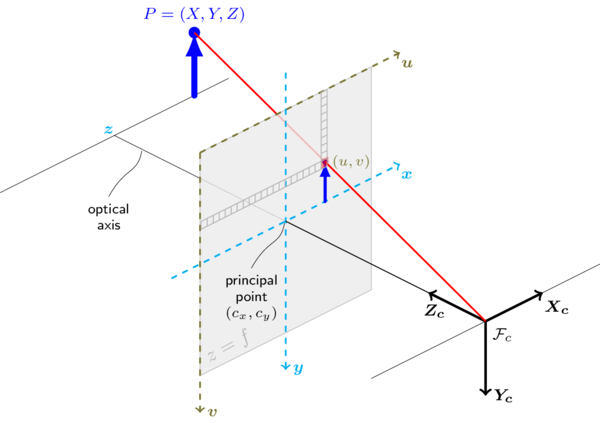
\includegraphics[width=0.7\linewidth]{figures/pinhole-camera-model.png}
	\caption{Diagram showing the parameters of the pinhole camera model. Source: INSERT}
	\label{fig:pinhole-camera-model}
\end{figure}

The intrinsic parameters of the camera can be expressed as a calibration matrix $\matr{K}$ defined as

\begin{equation}
	\matr{K}=
	\begin{bmatrix}
		f_x & s & c_x \\ 
		0 & f_y & c_y \\ 
		0 & 0 & 1
	\end{bmatrix}
	\label{eqn:calibration-matrix}
\end{equation}

The parameter $s$ in Equation \ref{eqn:calibration-matrix} captures the skew of the sensor axes that occurs as a result of the optical axis not being exactly perpendicular to the sensor plane. However, for practical purposes $s$ can be set to 0. Since the extrinsic parameters are captured by the rotation-translation matrix $[\matr{R}|\vect{t}]$, both the intrinsic and extrinsic parameters are captured by the product of this matrix and the calibration matrix $\matr{K}$. This 3 x 4 matrix product is referred to the camera matrix $\matr{P}$ and expressed mathematically as

\begin{equation}
	\matr{P}=\matr{K}[\matr{R}|\vect{t}].
	\label{eqn:camera-matrix}
\end{equation}

The camera matrix is sufficient to map the world coordinate system to the the image coordinate plane provided that the pinhole camera model is used and no lens distortion effects are present. This mapping is defined as

\begin{equation}
	s
	\begin{bmatrix}
		u \\ 
		v \\ 
		1
	\end{bmatrix}
	=
	\matr{P}
	\begin{bmatrix}
		X \\ 
		Y \\ 
		Z \\
		1
	\end{bmatrix}
	\label{eqn:pinhole-camera-mapping}
\end{equation}

where $(X,Y,Z)$ are the coordinates of a given point in the world coordinate system $\vect{p}^w$, $(u,v)$ are the coordinates of the corresponding point in the image coordinate system $\vect{p}^i$ and $s$ is simply a scaling factor. It is noted there is a loss of depth information when mapping from the world frame to the image frame. This is observed mathematically in Equation \ref{eqn:pinhole-camera-mapping} since $\matr{P}$ is not a square matrix and not invertible as a result. Therefore it is not possible to map from the image frame to the world frame without an additional piece of information. It was postulated that this piece of information could be obtained given that the length of the cube edge is known in the world frame. However, the cube side length differential was not found to be sufficiently large between vertical layers to make this distinction. Instead it was decided to provide the z coordinate of $\vect{p}^w$ based on the horizontal plane layer a cube was expected to be detected in. This is reasonable given that a cube dropped away from the source and structural cubes will always be found on the base plane.

In order to solve for the the world coordinates given the image coordinates, camera matrix $\matr{K}$ and world coordinate plane $Z$ using the pinhole camera model, Equation \ref{eqn:pinhole-camera-mapping} is expanded and rearranged as

\begin{equation}
	s
	\begin{bmatrix}
		u \\ 
		v \\ 
		1
	\end{bmatrix}
	=
	\matr{K}\left(\matr{R}
	\begin{bmatrix}
		X \\ 
		Y \\ 
		Z
	\end{bmatrix}
	+ \vect{t}\right),
	\label{eqn:expanded-pinhole-camera-mapping1}
\end{equation}

\begin{equation}
	\matr{R}^{-1}\matr{M}^{-1}
	s
	\begin{bmatrix}
		u \\ 
		v \\ 
		1
	\end{bmatrix}
	=
	\begin{bmatrix}
		X \\ 
		Y \\ 
		Z
	\end{bmatrix}
	+ \matr{R}^{-1}\vect{t}.
	\label{eqn:expanded-pinhole-camera-mapping2}
\end{equation}

In order to solve for the unknown scaling factor $s$, the intermediate vectors $\vect{x}$ and $\vect{y}$ are defined as

\begin{equation}
	\vect{x}=
	\begin{bmatrix}
		x_1 \\ 
		x_2 \\ 
		x_3
	\end{bmatrix}
=
	\matr{R}^{-1}\matr{M}^{-1}
	\begin{bmatrix}
		u \\ 
		v \\ 
		1
	\end{bmatrix},
	\label{eqn:expanded-pinhole-camera-mapping-left-matrix}
\end{equation}

\begin{equation}
	\vect{y}
	=
	\begin{bmatrix}
		y_1 \\ 
		y_2 \\ 
		y_3
	\end{bmatrix}
	=
	\matr{R}^{-1}\matr{t},
	\label{eqn:expanded-pinhole-camera-mapping-right-matrix}
\end{equation}

such that Equation \ref{eqn:expanded-pinhole-camera-mapping2} can be rewritten as

\begin{equation}
	s\,\vect{x}=
	\begin{bmatrix}
		X \\ 
		Y \\ 
		Z
	\end{bmatrix}
	+\vect{y}.
	\label{eqn:expanded-pinhole-camera-mapping-simplified}
\end{equation}

Since the camera matrix $\matr{P}$ is given, the rotation matrix $\matr{R}$, translation matrix $\vect{t}$ and intrinsic matrix $\matr{M}$ in Equations \ref{eqn:expanded-pinhole-camera-mapping-left-matrix} and \ref{eqn:expanded-pinhole-camera-mapping-right-matrix} are known. Consequently, $s$ can be computed as

\begin{equation}
	s=\frac{Z+y_3}{x_3}.
	\label{eqn:expanded-pinhole-camera-mapping-scaling-factor}
\end{equation}

Finally, with $s$ known, it is trivial to make use of Equation \ref{eqn:expanded-pinhole-camera-mapping-simplified} to obtain the world coordinates. For completeness, this is expressed as

\begin{equation}
	\begin{bmatrix}
		X \\ 
		Y \\ 
		Z
	\end{bmatrix}=
	s\,\vect{x}-\vect{y}.
	\label{eqn:expanded-pinhole-camera-mapping-final}
\end{equation}

% TODO: Insert C++ implementation of the project image point function

%Therefore, in order to map the centroids of the cubes from the image coordinate space to the world coordinate space, the intrinsic and extrinsic parameters of the camera need to be determined. Furthermore, real world cameras have lens distortion effects that need to be adjusted for. The OpenCV library was used to perform this camera calibration process to produce the intrinsic parameters of the camera. Furthermore, in order to account for the lens distortion, an improved intrinsic matrix was computed. It must be noted that most literature identifies the camera matrix $P$ as a product of the intrinsic and extrinsic matrices. However, OpenCV refers to the intrinsic matrix $K$ as the camera matrix. 
%
%In order to perform the camera calibration process and account for the lens distortion, 35 images were taken of a 8x6 checkerboard at various positions and orientations within the camera's FOV such as shown in Figure X. Various known points were subsequently identified on the checkerboard as shown in X to facilitate computation of the camera matrix. The improved camera matrix as well as the distortion coefficients describing the tangential and radial lens distortion are used to remap a distorted image as shown in Figure X as to remove the distortion. The undistorted image is shown in Figure X. Note how the checkerboard lines are perfectly aligned with the red ground truth lines while they are compressed inwards in the distorted image in Figure X.

In order to make use of the mathematical tools discussed above, the intrinsic parameters and extrinsic parameters of the camera needed to be determined. The intrinsic parameters were determined using a checkerboard calibration. A number of images of the checkerboard were captured at various poses in the robotic subsystem's workspace. The \textit{findChessboardCorners}, \textit{calibrateCamera} and \textit{getOptimalNewCameraMatrix} OpenCV library functions were used in the camera calibration process. The camera's extrinsic parameters were obtained using the EP\textit{n}P variation of the \textit{solvePnP} function from the OpenCV library which serves as a solution to the P\textit{n}P problem. This requires point correspondences which refers to points that have a known location in both the image frame and the world frame. Given at least four of these points, it is possible to estimate the rotation and translation matrices.

% TODO: Possibly insert calibration images

\subsubsection{Top-Level Design} \label{sec:Top-Level Design}

The \textit{System Controller} maintains a non-probabilistic belief state for the location and orientation of each cube with respect to the robot's coordinate system. Furthermore, four mutually exclusive states are used to distinguish between cubes. A \textit{source cube} is a cube that is believed to be in its known initial position while a \textit{structure cube} is believed to have been successfully placed in its designated position within the 3D shape under construction. If no unexpected events occur during the construction process, each cube will only exist in either of one these two states. The two unexpected events the system is expected to deal with are the dropped cube case and the structural damage case. If the vacuum system pressure sensor detects that a cube is dropped during manipulation by the robot, the cube is classified as a \textit{missing cube}. A cube that is detected by the \textit{Vision System} that is not in an expected \textit{source cube} or \textit{structure cube} location is classified as an \textit{independent cube}. The \textit{System Controller} is able to deal with both the dropped cube case and the structural damage case when the position and orientation of all \textit{independent cubes} with respect to the robot's coordinate system are provided. This is discussed in greater detail in Section <INSERT>. As such, the purpose of the \textit{Vision System} is to detect and localise all \textit{independent cubes} with respect to the robot given the image input data of the robot's workspace. The expected location of the \textit{source cubes} and the \textit{structure cubes} with respect to the robot for a given time instance are also required as input to distinguish these cubes from the \textit{independent cubes}.

% TODO: Possibly insert cube state diagram

\begin{figure}[!ht]
	\centering
	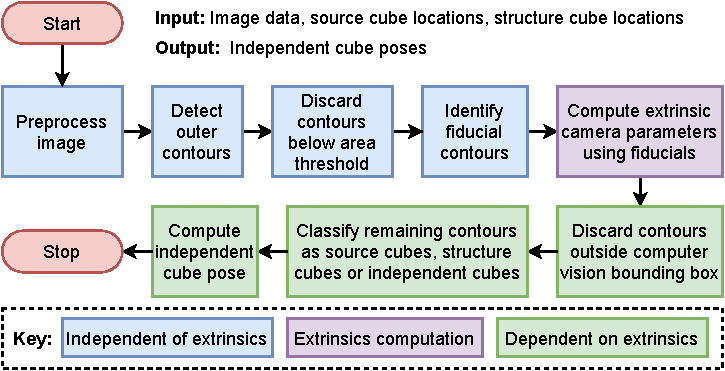
\includegraphics[scale=1]{figures/high-level-computer-vision-design.pdf}
	\caption{Flow diagram showing the steps in the integrated computer vision process.}
	\label{fig:high-level-computer-vision-design}
\end{figure}

Figure \ref{fig:high-level-computer-vision-design} shows the high level steps the \textit{Vision System} performs each time it is instructed to process the image input data captured by the camera. The findings from the cube feature investigation performed in Section \ref{sec:Cube Feature Investigation} guided the design of this process. The input image is expected to be in RGB color format and may be of arbitrary size.  A preprocessing step is applied to the image in which the image is first converted to grey-scale format. This is followed by the application of a Gaussian blur function to eliminate high-frequency noise within the image that appears as local outlier pixel intensities. Finally, a fixed binary threshold is applied to the image as the initial step to segment the top faces of the cube, as discussed in Section \ref{sec:Cube Feature Investigation}. This step also segments the fiducial markers, the design of which are discussed later in Section \ref{sec:Fiducial Identification}.

Following the preprocessing step, contour detection is applied to the binary image to convert the connected 1-components within the image to a discrete set of elements that can be processed individually. The cubes and fiducials are assumed to be surrounded by the plain black background of the robot's base plane and, as such, only the outer contours are detected to ensure the patterns within the fiducial are not identified as separate elements to the fiducial. Finally, a number of contours originating from image artifacts that are not cubes or fiducials are also detected as part of this step. In order to reduce the amount of processing required during later contour classification steps, the area enclosed by each contour is computed and all contours with an area significantly smaller than that of cubes and fiducials on the base plane are discarded.

% TODO: Insert raw image and image after binary thresholding

With the set of fiducial and cube candidate contours compiled, the next phase of the algorithm is concerned with the classification of these contours. Firstly, the contours that enclose fiducial markers are identified as part of the fiducial identification step (see Section \ref{sec:Fiducial Identification}) which includes the extraction of the unique fiducial identifier values. The location of each fiducial in the world coordinate system is known and retrieved from a look-up table based on the fiducial identifier. The location of the fiducial within the image coordinate system is taken as the location of the fiducial contour centroid. With this information, a point correspondence between the world coordinate system and image coordinate system can be formed for each fiducial and used to compute the extrinsic camera parameters as discussed in Section \ref{sec:3D Localisation}. Furthermore, the methods to map between the image frame and world frame may now be used with the camera extrinsics calibrated. The base plane of the robot was controlled such that the workspace only contains cubes and fiducials. By restricting the remaining contours under consideration to only those that are detected within the robot's workspace, these contours are guaranteed to be artifacts of construction cubes since the fiducial contours have already been identified.

The rectangular bounding region of the robot's workspace is aligned with the world coordinate system. As such, it is trivial to determine if a point falls within this region if the point is also defined in the world frame. Therefore, to determine if the centroid point of a given contour in the image frame falls within the bounding region, the point is first projected to the world coordinate system using Equation \ref{eqn:expanded-pinhole-camera-mapping-final}. As noted in section \ref{sec:3D Localisation}, when projecting from image space to world space, it is necessary to specify the $Z$ plane of projection in the world frame. Since the camera captured images from the vertical perspective, it was considered sufficient to project the contour centroids to the base plane, $Z=0$. Following this step, all contours with centroids external to the bounding region are discarded.

With the remaining contours assumed to only be image artifacts originating from cubes, the contours need to be classified as either \textit{source cube}, \textit{structure cube} or \textit{independent cube} contours. This classification is based on expected locations of the \textit{source cubes} and \textit{structure cubes} in the world frame as provided to the \textit{Vision System} by the \textit{System Controller}. For the \textit{source cubes}, the proximity of the centroid of each contour to the centre of the top face of each \textit{source cube} is considered. If the contour centroid is considered sufficiently close\footnote{A centroid is considered sufficiently close to the centre of the top cube face if the Euclidean distance between these points is less than one cube side length.} to the top face centre of any of the \textit{source cubes}, the contour is considered to be a \textit{source cube} contour. The same applies for \textit{structure cubes}. To facilitate the proximity calculations, the contour centroid is projected to the world coordinate system for each cube the contour is compared with using Equation\ref{eqn:expanded-pinhole-camera-mapping-final}. The $Z$ coordinate of the top face of the cube under consideration is used as the $Z$ plane of projection in the world frame. The world frame Euclidean distance between the projected centroid point and the cube top face centre is computed as the measure of their proximity. If a contour is classified as neither a \textit{source cube} nor a \textit{structure cube} contour, it is assumed to be an \textit{independent cube} contour. Finally, The orientation and location of each detected \textit{independent cube} is estimated as outlined in Section \ref{sec:Cube Pose Estimation}.

% TODO: Insert the final image processing image

\subsubsection{Fiducial Identification} \label{sec:Fiducial Identification}

The location of the fiducials within the image input data provide the corresponding image frame coordinates to the known world coordinates of the fiducials to form point correspondences. It has been found that a greater number of point correspondences generally leads to an improved solution to the P\textit{n}P problem. As such, eight fiducial markers were placed at eight known locations on the robot's base plane. Each fiducial was structured as a square with a white border with an imaginary internal grid of 3x3 squares each having a side length of 5mm. The black squares were defined to represent a binary zero and the white squares a binary one. In order to ensure the rotation of the fiducial can be uniquely determined, the squares at coordinates $(0, 0)$, $(2, 0)$ and $(2,2)$ were assigned the binary values of 0, 0 and 1 respectively. The six remaining binary squares facilitated the representation of $2^6=64$ unique identifiers. Figure \ref{fig:fiducial-step1} shows an example of a fiducial marker located on the robot's base plane. 

\begin{figure}[!ht]
	\centering
	\begin{subfigure}{.24\textwidth}
		\centering
		
\includegraphics[width=0.8\linewidth]{figures/fiducial-step1}
		\caption{Original}
		\label{fig:fiducial-step1}
	\end{subfigure}%
	\begin{subfigure}{.24\textwidth}
		\centering
		
\includegraphics[width=0.8\linewidth]{figures/fiducial-step2}
		\caption{Isolated}
		\label{fig:fiducial-step2}
	\end{subfigure}
	\begin{subfigure}{.24\textwidth}
		\centering
		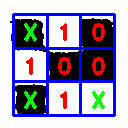
\includegraphics[width=0.8\linewidth]{figures/fiducial-step3}
		\caption{Processed}
		\label{fig:fiducial-step3}
	\end{subfigure}
	\begin{subfigure}{.24\textwidth}
		\centering
		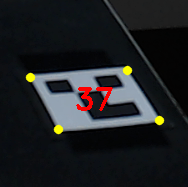
\includegraphics[width=0.8\linewidth]{figures/fiducial-step4}
		\caption{Annotated}
		\label{fig:fiducial-step4}
	\end{subfigure}
	\caption{Various stages of fiducial detection and identification in the computer vision subsystem.}
	\label{fig:fiducial-stages}
\end{figure}

The fiducial identification step takes place after the contour extraction phase shown in Figure \ref{fig:high-level-computer-vision-design}. The purpose of this step is to identify which of the detected contours are an artifacts of fiducials, to acquire the image coordinates of the fiducials and to extract the fiducial identifiers. An overview of the fiducial identification algorithm developed for this project is shown in Figure \ref{fig:fiducial-identification}. This algorithm follows the approach of initially assuming that each contour is a fiducial and discarding contours in latter steps if the contour does not fulfill certain fiducial requirements. Following this logic, the four corners of the fiducial candidate contour are extracted using the algorithm presented in later Section \ref{sec:Square Corner Detection} based on the assumption that the contour is a square. Using the detected corners, the internal angles and side lengths of this quadrilateral are computed. If they do not approximate the properties of a square, the contour is discarded.

\begin{figure}[!ht]
	\centering
	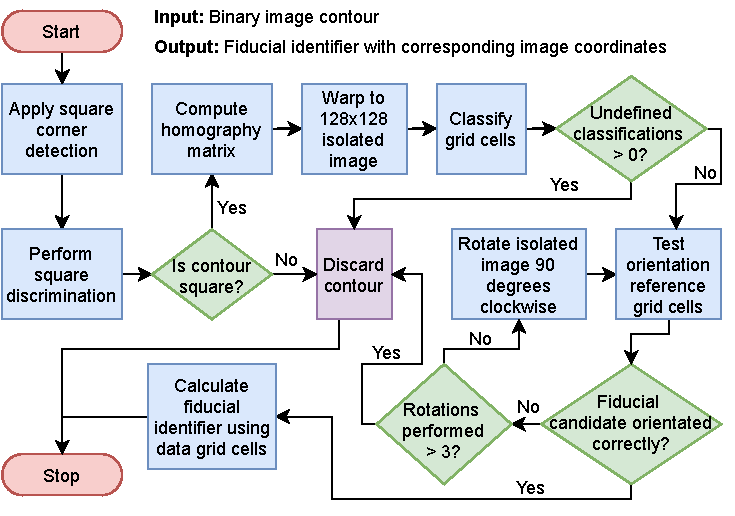
\includegraphics[scale=1]{figures/fiducial-identification.pdf}
	\caption{Flow diagram showing the steps in the fiducial identification process.}
	\label{fig:fiducial-identification}
\end{figure}

It was noted that the fiducial in the image captured by the camera has a degree of perspective warping compared to the reference digital fiducial image. In order to correct for this perspective warp, a 3x3 homography matrix $\matr{H}$ is computed using the \textit{findHomography} OpenCV library function. Four point correspondences are required to compute $\matr{H}$. These correspondences are obtained by arbitrarily pairing each of the fiducial candidate's detected corner coordinates in the original image to the corner coordinates of a 128 x 128 pixel destination image. The fiducial candidate region in the original image is warped to the destination image such that the fiducial pattern is isolated as shown in Figure \ref{fig:fiducial-step2}. The internal region of the isolated fiducial candidate image is divided into a pre-placed 3x3 grid of squares corresponding to the expected positions of the fiducial squares. This grid is shown in Figure \ref{fig:fiducial-step3}. For the grid cell to be classified as a binary one or zero, at least 75\% of the inner 30 x 30 pixels of the square need to have a pixel intensity of 255 or 0 respectively. If the condition is not met for either value for any grid cell, the grid cell is considered unclassified and the contour is discarded.

Once all the grid cells have been classified, the orientation reference cells at $(0, 0)$, $(2, 0)$ and $(2,2)$ are compared with the expected binary values of 0, 0 and 1 respectively. If these match, the fiducial is considered to be correctly oriented. Otherwise, the isolated fiducial candidate is rotated 90$^{\circ}$ clockwise until the correct orientation is found. If the correct orientation is not found after three rotations have been performed, the contour is discarded. Finally the unique binary identifier encoded in the fiducial is extracted by reading the binary values of the cells from left to right and top to bottom excluding the orientation cells. The cells are ordered from the least significant bit (LSB) to the most significant bit (MSB). Figure \ref{fig:fiducial-step3} shows the result of applying the fiducial identification step to the isolated fiducial in Figure \ref{fig:fiducial-step3}. The orientation reference cells are indicated by green crosses while the fiducial has been rotated to align with these cells. The binary values detected in each cell are indicated in red. In this case the identifier is calculated as $100101_2=37$. The fiducial in the original image is annotated with the detected corners as well as the fiducial identifier as shown in Figure \ref{fig:fiducial-step4}.

%\begin{figure}[H]
%	\centering
%	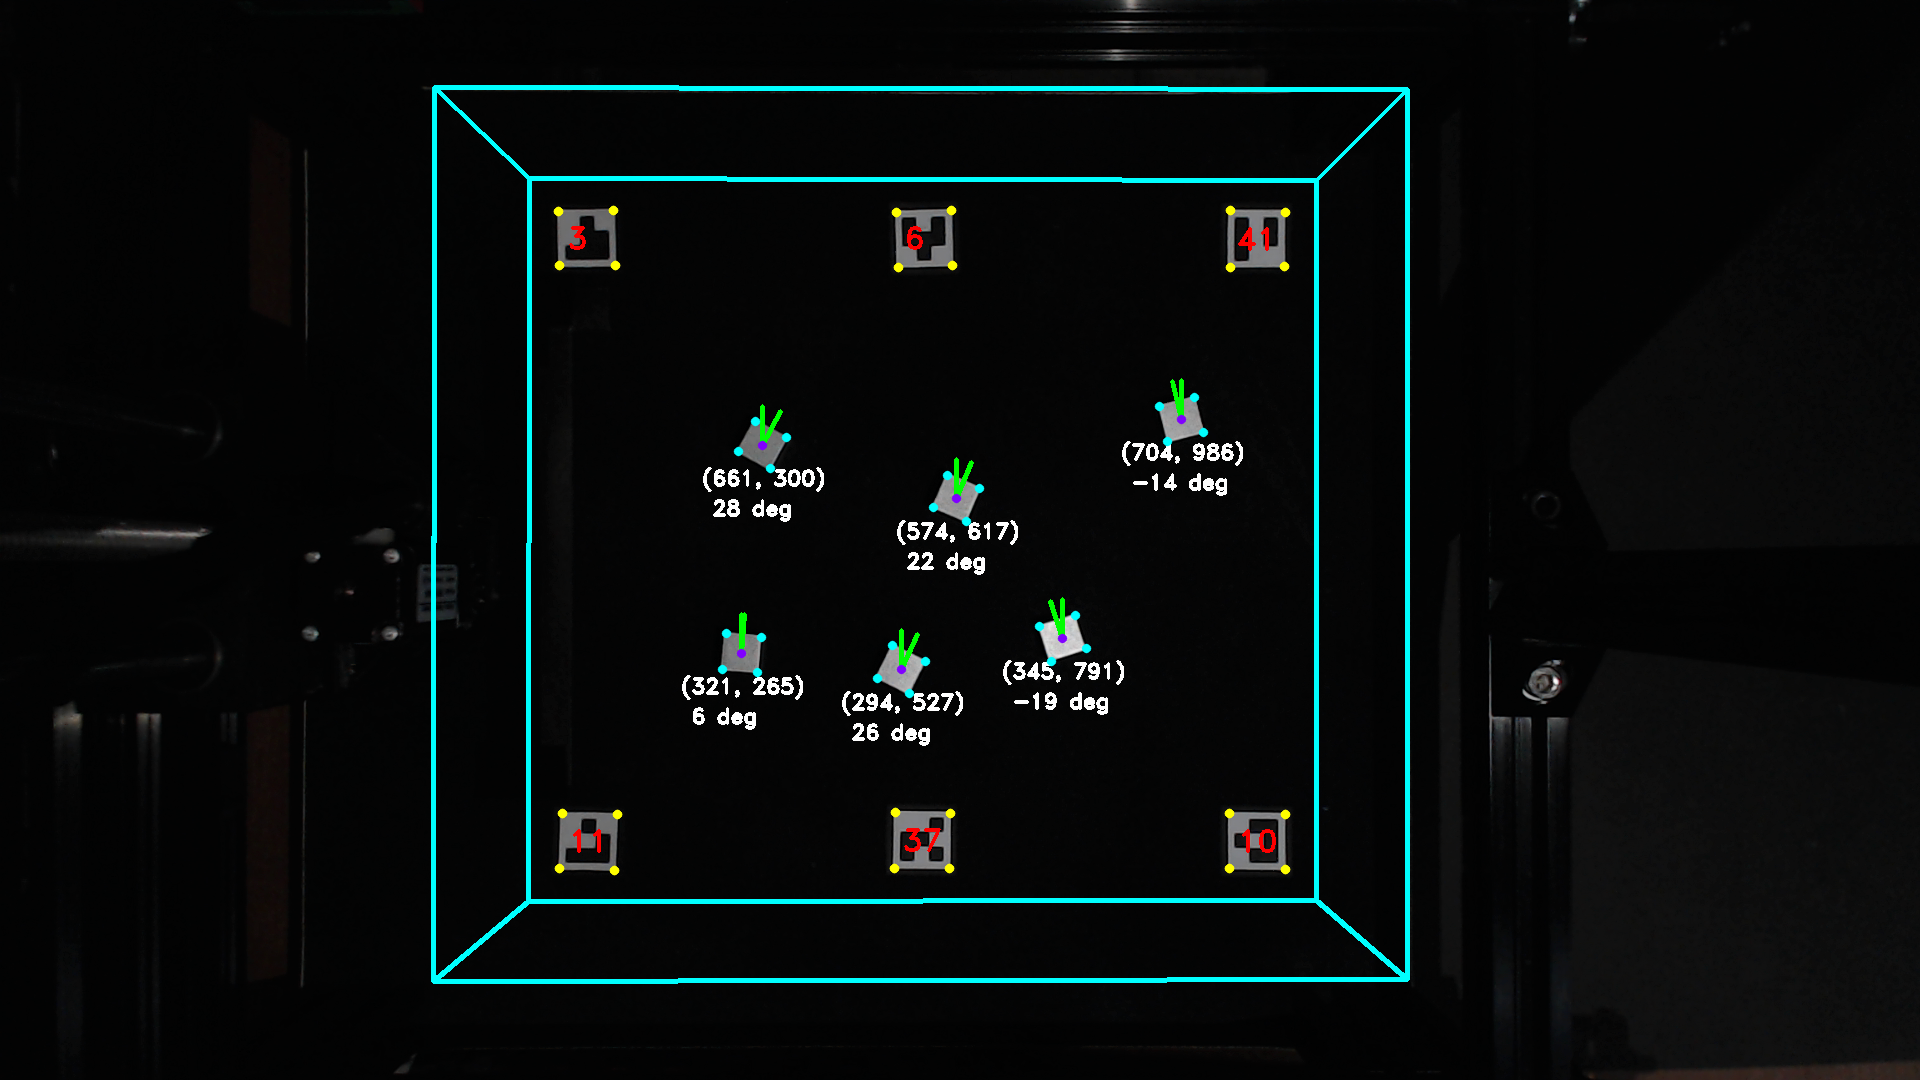
\includegraphics[width=1\linewidth]{figures/computer-vision-overview.png}
%	\caption{Screen capture of the desktop software component showing the fiducial detection, cube detection and bounding box visualisation aspects of the computer vision system.}
%	\label{fig:computer-vision-overview}
%\end{figure}

\subsubsection{Square Corner Detection} \label{sec:Square Corner Detection}

Both the fiducial identification (see Section \ref{sec:Fiducial Identification}) and cube orientation computation (see Section \ref{sec:Cube Pose Estimation}) algorithms require the corners of the contours to be known in the image coordinate system. It was decided to extract these corners from a given contour based on the assumption that the underlying shape is a square. The first step in the corner detection process is the computation of the centroid of the contour. Following this, the Euclidean distances between the centroid and each of the contour points are computed. The contour point that has the greatest Euclidean distance from the centroid is taken to be the first corner. The remaining contour points are then segmented into four quadrants with the origin of the quadrant axes coincident with the centroid of the contour and the axes oriented such that the detected corner falls at the centre of the first quadrant. This is based on the fact that the four corners of a square can be separated into four quadrants. The contour points with the greatest Euclidean distance from the centroid in each of the remaining three quadrants are taken to be the remaining three corners.

% TODO: Insert diagram showing corner detection sequence

\subsubsection{Cube Pose Estimation} \label{sec:Cube Pose Estimation}

From a black box perspective, the cube pose estimation step in this project takes the contour of the top face of a cube as input and produces an estimate of the orientation and location of the cube with respect to the world coordinate system as output. The location of the centre of the top face of the cube in the world coordinate system is obtained through the projection of the centroid of the cube contour from the image coordinate system using Equations \ref{eqn:expanded-pinhole-camera-mapping-scaling-factor} and \ref{eqn:expanded-pinhole-camera-mapping-final}. The $Z$ plane of projection in the world coordinate system needs to be specified as part of this step. Since only \textit{independent cubes} need to be localised as discussed in Section \ref{sec:Top-Level Design}, it is assumed the cube to be localised always be on the base plane. This is reasonable as \textit{independent cubes} only exist as the result of an unexpected event such as the dropped cube event in which case the \text{independent cube} will always be on the base plane. Therefore, for projection purposes, the $Z$ plane of projection is defined as the $Z$ position of the top-face of a cube on the base plane. In other words, the $Z$ plane of projection is one cube side length above the base plane.

Under normal circumstances, every cube in the robot's workspace will always have a face parallel to the base plane. Therefore, the detection of the orientation of a cube with respect to the world frame is reduced to the detection of rotation of the cube about the z-axis. Specifically, this rotation is defined as the angle between the positive x-axis in the world frame and the perpendicular line from any cube edge to the centre of the top face of the cube. Furthermore, since the top face of the cube is a square which has rotational symmetry of order 4 and a 90$^{\circ}$ angle of rotational symmetry, the rotational angle range of the cube is mapped to the range $(45^{\circ},45^{\circ}]$. The centroid and the four square corners of the cube contour are used to estimate the orientation of the cube. Since the square corners are already computed for each salient contour in the fiducial identification step (see Section \ref{sec:Fiducial Identification}), this result is simply reused for the relevant contours in this step.

Since the corners are defined with respect to the image frame, they are also projected to the same $Z$ plane as the contour centroid projected initially. The coordinates of the centroid and four corners in the world $Z$ plane are used to compute the rotation of the cube. There are four lines, each between a corner and the centroid, that can be used to form an angle with the positive x-axis. By computing the angle using each of these lines separately, the average estimated angle can then be computed with reduced high-frequency noise. However, an average angle cannot be computed through the sum and normalisation of the angle data as this is incorrect mathematically. Instead, one of the lines is chosen as a reference while the three corners are rotated by either -90$^{\circ}$,  90$^{\circ}$ or  180$^{\circ}$ to be in the same quadrant as the reference line. The average line position is computed by taking the average X and Y position of the rotated corners and this can be used to calculate the average estimated angle with respect to the positive x-axis. Finally, since the cube orientation is defined using a perpendicular line to the nearest edge, 22.5$^{\circ}$ is added to the estimated angle to account for the fact a corner line was used to compute the average angle. Finally, this angle is mapped to the range $(45^{\circ},45^{\circ}]$.

% TODO: Possibly add algorithm step graphcis
% TODO: Add cube orientation annotation close up

\subsection{System Controller} \label{sec:System Controller}

The core requirements that the PC-based software needed to fulfil are as follows:

\begin{compactitem}
	\item The software needs to capture the desired 3D shape to be constructed from the user.
	\item The software needs to provide a visualisation of the shape to be constructed to the user to verify the captured shape is correct.
	\item The software needs to interface with the camera hardware to receive the image input data from the camera.
	\item The software needs to process the image data to detect and localise the cubes input image data.
	\item The software needs to display the raw and annotated camera image data to the user to show the image processing functionality to the user.
	\item The software needs to the utilise the 3D shape input information in conjunction with the processed image information to generate instructions for the robot to construct the 3D shape.
	\item The software needs to convert the robot instructions into a format corresponding to the serial communication protocol between the robot and the computer before sending this data to the robot.
	\item The software needs to monitor the status of the robotic subsystem based on data received from the robot.
	\item The software needs to support the initialisation of the necessary system qualification tests.
\end{compactitem}

\subsubsection{Construction Planner}

\ldots

\subsubsection{Robotic Motion Planner}

\ldots

\subsubsection{Integration}

\ldots

\newpage

%% End of File.


%%
%%  Department of Electrical, Electronic and Computer Engineering.
%%  EPR400/2 Final Report - Section 4.
%%  Copyright (C) 2011-2021 University of Pretoria.
%%

\section{Results}

\subsection{Summary of results achieved}

\begin{table}[H]
	\renewcommand{\arraystretch}{1.3}
	\centering
	\begin{tabular}{|>{\raggedright}m{6.5cm}|>{\raggedright}m{5cm}|>{\raggedright\arraybackslash}m{2.2cm}|}
		\hline
		\textbf{Intended outcome} & \textbf{Actual outcome} & \textbf{Location in report} \\
		\hline
		\multicolumn{3}{|l|}{\textbf{Core mission requirements and specifications}} \\
		\hline
		The system should construct novel and moderately complex 3D shapes using small cubes. The system should handle shapes up to at least 4 cubes in height containing up to at least 30 cubes where each cube has a face parallel to the base plane. The system should handle equal size cubes with a side length between 10mm and 15mm. & & Section 4.2.1 \\
		\hline
		The GUI should allow the user to define a wide range of 3D shapes to be constructed. For each constituent cube in the shape, the GUI should allow the position of each cube to be specified along each Cartesian axis with at least 1mm resolution as well as the rotation of each cube about the z-axis with at least 1 degree resolution. & & Section 4.2.2 \\
		\hline
		The end-effector should be able to grip a cube, maintain its grip during motion and release the cube. The end-effector should maintain the cube in its grip when the robotic manipulator is at maximum acceleration. The end-effector should be able to maintain the cube in its grip for at least 20 seconds continuously. &  & Section 4.2.3 \\
		\hline
	\end{tabular}
	\caption{\label{tab:results_summary_p1}Summary of results achieved.}
\end{table}

\begin{table}[H]
	\renewcommand{\arraystretch}{1.3}
	\centering
	\begin{tabular}{|>{\raggedright}m{6.5cm}|>{\raggedright}m{5cm}|>{\raggedright\arraybackslash}m{2.2cm}|}
		\hline
		\textbf{Intended outcome} & \textbf{Actual outcome} & \textbf{Location in report} \\
		\hline
		\multicolumn{3}{|l|}{\textbf{Core mission requirements and specifications}} \\
		\hline
		The robotic manipulator should accurately translate the end-effector in 3D space and rotate it about its vertical axis. The robotic manipulator should have a repeatability of at least 2mm for each Cartesian axis and a repeatability of at least 5 degrees for the rotation about the z-axis. & & Section 4.2.4 Section 4.2.5 \\
		\hline
		The computer vision component should detect and localise the construction cubes in the workspace to facilitate re-gripping dropped cubes and identifying damage to the 3D shape under construction to signal a construction halt condition. Only the cubes whose faces are visible from a vertical perspective need to be detected and localised. Cubes that need to be gripped should be localised with a positional accuracy of 2mm and a rotational accuracy of 5 degrees about the z-axis. & & Section 4.2.6 Section 4.2.7 \\
		\hline
		The system should detect when a cube is unintentionally dropped by the end-effector. The system should detect a cube has been dropped before the end-effector grips the next cube to be placed. & & Section 4.2.7 \\
		\hline
	\end{tabular}
	\caption{\label{tab:results_summary_p2}Summary of results achieved.}
\end{table}

\begin{table}[H]
	\renewcommand{\arraystretch}{1.3}
	\centering
	\begin{tabular}{|>{\raggedright}m{6.5cm}|>{\raggedright}m{5cm}|>{\raggedright\arraybackslash}m{2.2cm}|}
		\hline
		\textbf{Intended outcome} & \textbf{Actual outcome} & \textbf{Location in report} \\
		\hline
		\multicolumn{3}{|l|}{\textbf{Field condition requirements and specifications}} \\
		\hline
		The system should work under laboratory conditions. The ambient lighting level should be approximately 500 lux. & & Section 4.2.6 \\
		\hline
		The image background should be controlled. The immediate background of the construction cubes in the captured images should be non-reflective and of a single hue.& & Section 4.2.6 \\
		\hline
	\end{tabular}
	\caption{\label{tab:results_summary_p3}Summary of results achieved.}
\end{table}

\subsection{Qualification Tests}

This section presents the set of qualification tests that were performed to demonstrate conformance of the overall system, and various subsystems, to the system specifications. Prior to the commencement of a number of the qualification tests, the following setup steps, hereafter referred to as the \textit{General System Initialisation} procedure, must have been completed:

\begin{compactenum}
	\item Ensure robotic manipulator's workspace is completely empty.
	\item Power on the PC that will run the system control software.
	\item Ensure the system camera has a clear view of the system workspace and connect the camera to the PC.
	\item Connect the \textit{Robotic subsystem} to the PC by connecting the micro USB port on the embedded robot controller to a USB Type A port on the PC using a USB Type A to micro USB connector cable.
	\item Power on the robotic subsystem by connecting the power supply to a main's electricity outlet.
	\item Start the system control software on the PC.
	\item On the home screen in the system control software, verify the correct camera feed is displayed in the camera view.
	\item On the same screen, select the \textit{USB-Serial CH340} port from the available ports list.
	\item On the same screen, click the \textit{Connect to Robot} button and verify the robot is connected.
	\item Select the \textit{Construction} view in the system control software.
	\item Initialise calibration of the robot by clicking the \textit{Calibrate} button and verify the calibration sequence completes successfully.
\end{compactenum}

<INDICATE 3D TEST SHAPES ARE SPECIFIED IN APPENDIX>

\textbf{Qualification Test 1: Test of the system's capability to build 3D shapes}

\textit{Objectives of the test or experiment}

The aim of this test is to determine if the system is capable of constructing a variety of novel and moderately complex 3D shapes using small cubes each with a side length of between 10mm and 15mm. Novel and moderately complex 3D shapes constitute shapes containing up to at least 30 cubes where each cube has a face parallel to the base plane.

\textit{Equipment used}

The following equipment was used to execute this qualification test:

\begin{compactitem}
	\item PC,
	\item \textit{PC System} software,
	\item \textit{Robotic Subsystem},
	\item USB Type A to micro USB connector cable,
	\item Logitech C920 HD Pro Webcam,
	\item and 30 aluminium cubes with side lengths of 12.6mm $\pm$0.05mm.
\end{compactitem}

\textit{Test setup and experimental parameters}

The following steps were completed in preparation for this qualification test:

\begin{compactenum}
	\item Ensure the \textit{General System Initialisation} procedure has been completed.
	\item Navigate to the \textit{Construction} view in the system control GUI.
	\item Click on the \textit{Load model} button and verify the \textit{.cubeworld} test shape files are available for construction.
\end{compactenum}

\textit{Steps followed in the test or experiment}

The following steps were carried out to execute this qualification test:

\begin{compactenum}
	\item Clear the \textit{Robotic Subsystem's} workspace and place the 30 cubes at the pre-defined \textit{source cube} locations.
	\item Select and load a pre-defined test shape model in the \textit{Construction} view of the system control GUI using the \textit{Load Model} button.
	\item Verify the correct model is loaded in the 3D shape display.
	\item Start the construction process by clicking the \textit{Start Construction} button in the system control GUI and wait for the robotic subsystem to construct the shape.
	\item Compare the constructed shape to the selected test shape in the 3D shape display in the GUI and qualitatively classify the shape construction as either a success or failure.
	\item Repeat all the steps 1 to 5 of the experimental protocol with a different pre-defined test shape selected in step 2. 
	\item Repeat step 6 until all the pre-defined test shapes have been built.
\end{compactenum}

\textit{Results or measurements}

\ldots

\textit{Observations}

\ldots

\textit{Statistical analysis}

\ldots

\textbf{Qualification Test 2: Test of system's capability to facilitate the definition of 3D shapes}

\textit{Objectives of the test or experiment}

The aim of this test is to determine if the system is capable of capturing and representing a user-specified 3D shape where the position of each constituent cube is specified along each Cartesian axis as well as the orientation about the z-axis.

\textit{Equipment used}

The following steps were carried out to execute this qualification test:

\begin{compactitem}
	\item PC,
	\item and \textit{PC System} software.
\end{compactitem}

\textit{Test setup and experimental parameters}

The following steps were completed in preparation for this qualification test:
\begin{compactitem}
	\item Start the system control software on the PC.
	\item Navigate to the \textit{Shape Design} view in the system control GUI.
\end{compactitem}

\textit{Steps followed in the test or experiment}

The following steps were carried out to execute this qualification test:

\begin{compactenum}
	\item Click on the \textit{Insert Cube} button in the \textit{Shape Design} view in the system control GUI.
	\item Verify a cube is displayed in the 3D shape display.
	\item Record the displayed x-axis position value for the cube.
	\item Translate the cube one step in the positive x-axis direction.
	\item Record the displayed x-axis position value for the cube.
	\item Translate the cube one step in the negative x-axis direction
	\item Record the displayed x-axis position value for the cube.
	\item Repeat steps 2 to 6 for translation along the y-axis.
	\item Repeat steps 2 to 6 for rotation about the z-axis.
	\item Click on the \textit{Insert Cube} button
	\item Verify an additional cube is added to the 3D shape display.
	\item Verify the cube can be translated along the x-, y-, and z-axis and rotated about the z-axis.
	\item Repeat steps 10 to 12 until 30 cubes are displayed in the 3D shape display.
\end{compactenum}

\textit{Results or measurements}

\ldots

\textit{Observations}

\ldots

\textit{Statistical analysis}

\ldots

\textbf{Qualification Test 3: Test of end-effector's capability to manipulate cubes}

\textit{Objectives of the test or experiment}

The aim of this test is to determine if the end-effector is capable of maintaining a cube in its grip under motion when the robotic manipulator is at maximum acceleration. The test also aims to determine if the end-effector is able to maintain the cube in its grip for at least 20 seconds continuously and if it is able to grip and ungrip the cube.

\textit{Equipment used}

The following equipment was used to execute this qualification test:

\begin{compactitem}
	\item PC,
	\item \textit{PC System} software,
	\item \textit{Robotic Subsystem},
	\item USB Type A to micro USB connector cable,
	\item Digital stopwatch,
	\item and an aluminium cube with a side length of 12.6mm $\pm$0.05mm.
\end{compactitem}

\textit{Test setup and experimental parameters} 

The following steps were completed in preparation for this qualification test:

\begin{compactenum}
	\item Ensure the \textit{General System Initialisation} procedure has been completed.
	\item Navigate to the \textit{Construction} view in the system control GUI.
\end{compactenum}

\textit{Steps followed in the test or experiment}

The following steps were carried out to execute this qualification test:

\begin{compactenum}
	\item Place the cube in first position of the pre-defined \textit{source cube} locations.
	\item Click on the \textit{Execute QTP 3} button to initiate the robot's routine for this qualification test.
	\item Verify the robotic subsystem proceeds to locate and grip the cube placed during the test setup.
	\item Start the stopwatch as the cube is lifted off the base plane by the robotic manipulator.
	\item Verify, the robot continuously between the extreme locations on each axis.
	\item Stop the stopwatch and record the elapsed time if the cube is dropped by the robot at any point during the robot's movement sequence up to 30 seconds.
	\item After 30 seconds halt the robot's movement sequence and record if the cube is still gripped by the robot.
	\item Repeat steps 1 to 7 for a total of 10 iterations including the first iteration.
\end{compactenum}

\textit{Results or measurements}

\ldots

\textit{Observations}

\ldots

\textit{Statistical analysis}

\ldots

\textbf{Qualification Test 4: Measurement of robotic manipulator linear accuracy}

\textit{Objectives of the test or experiment}

The aim of this test is to determine the linear repeatability of the robotic manipulator's positioning along each Cartesian axis.

\textit{Equipment used}

The following equipment was used to execute this qualification test:

\begin{compactitem}
	\item PC,
	\item \textit{PC System} software,
	\item ImageJ image processing and analysis software,
	\item \textit{Robotic Subsystem},
	\item USB Type A to micro USB connector cable,
	\item Vertical flat-faced stand (see Figure \ref{fig:qtp4-z-axis-test-structure}),
	\item 2 sheets of plain white A4 paper,
	\item Digital caliper,
	\item 0.5mm Mechanical pencil,
	\item Electrical tape,
	\item and a Digital camera.
\end{compactitem}

\textit{Test setup and experimental parameters}

\begin{compactenum}
	\item Ensure the \textit{General System Initialisation} procedure has been completed.
	\item Navigate to the \textit{Construction} view in the system control GUI.
	\item Attach the mechanical pencil vertically and securely to the robot's \textit{End-Effector Assembly} using electrical tape as shown in Figure \ref{fig:qtp4-vertical-pencil}.
	\item Place the two sheets of plain white A4 paper on the base plane of the robot's workspace such that entire plane accessible by mechanical pencil tip is covered.
	\item Secure the paper sheets in place to the base plane using electrical tape.
\end{compactenum}

\begin{figure}[!ht]
	\centering
	\begin{subfigure}{.25\textwidth}
		\centering
		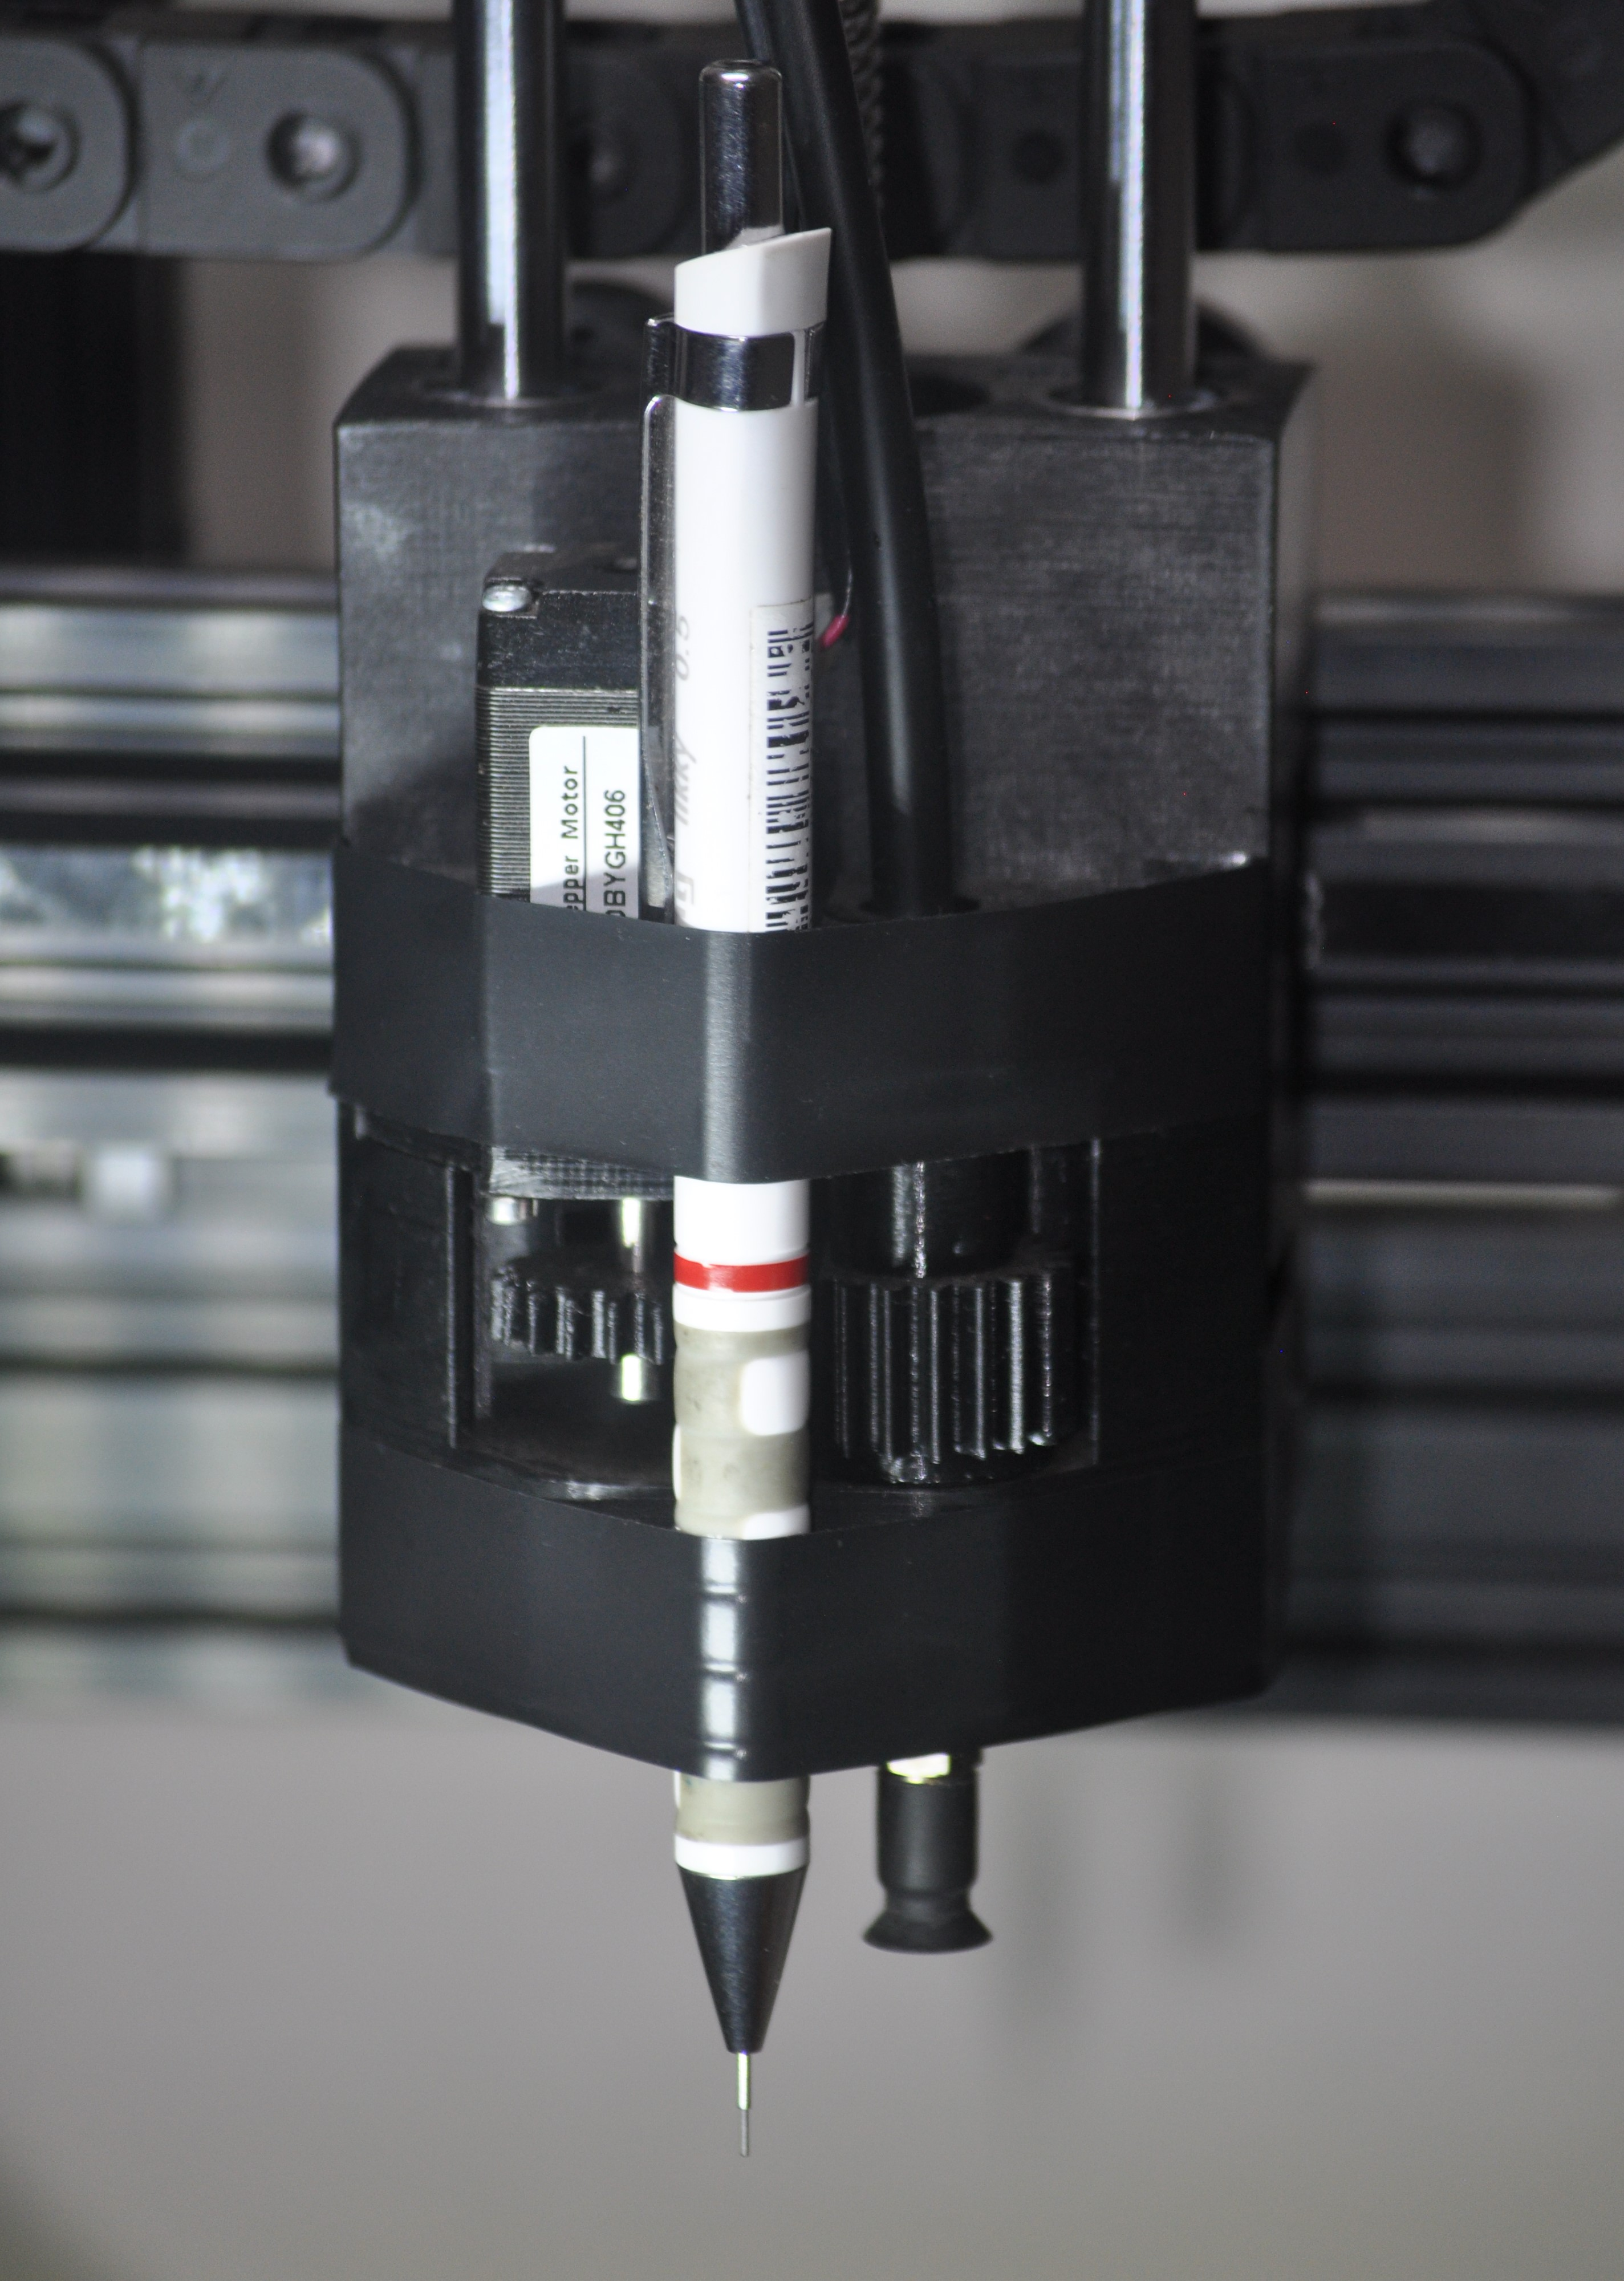
\includegraphics[width=0.95\linewidth]{figures/qualification-test-vertical-pencil.jpg}
		\caption{Vertical pencil}
		\label{fig:qtp4-vertical-pencil}
	\end{subfigure}%
	\begin{subfigure}{.53\textwidth}
		\centering
		\includegraphics[width=0.95\linewidth]{figures/qualification-test-horizontal-pencil.jpg}
		\caption{Horizontal pencil attachment}
		\label{fig:qtp4-horizontal-pencil}
	\end{subfigure}
	\begin{subfigure}{.21\textwidth}
		\centering
		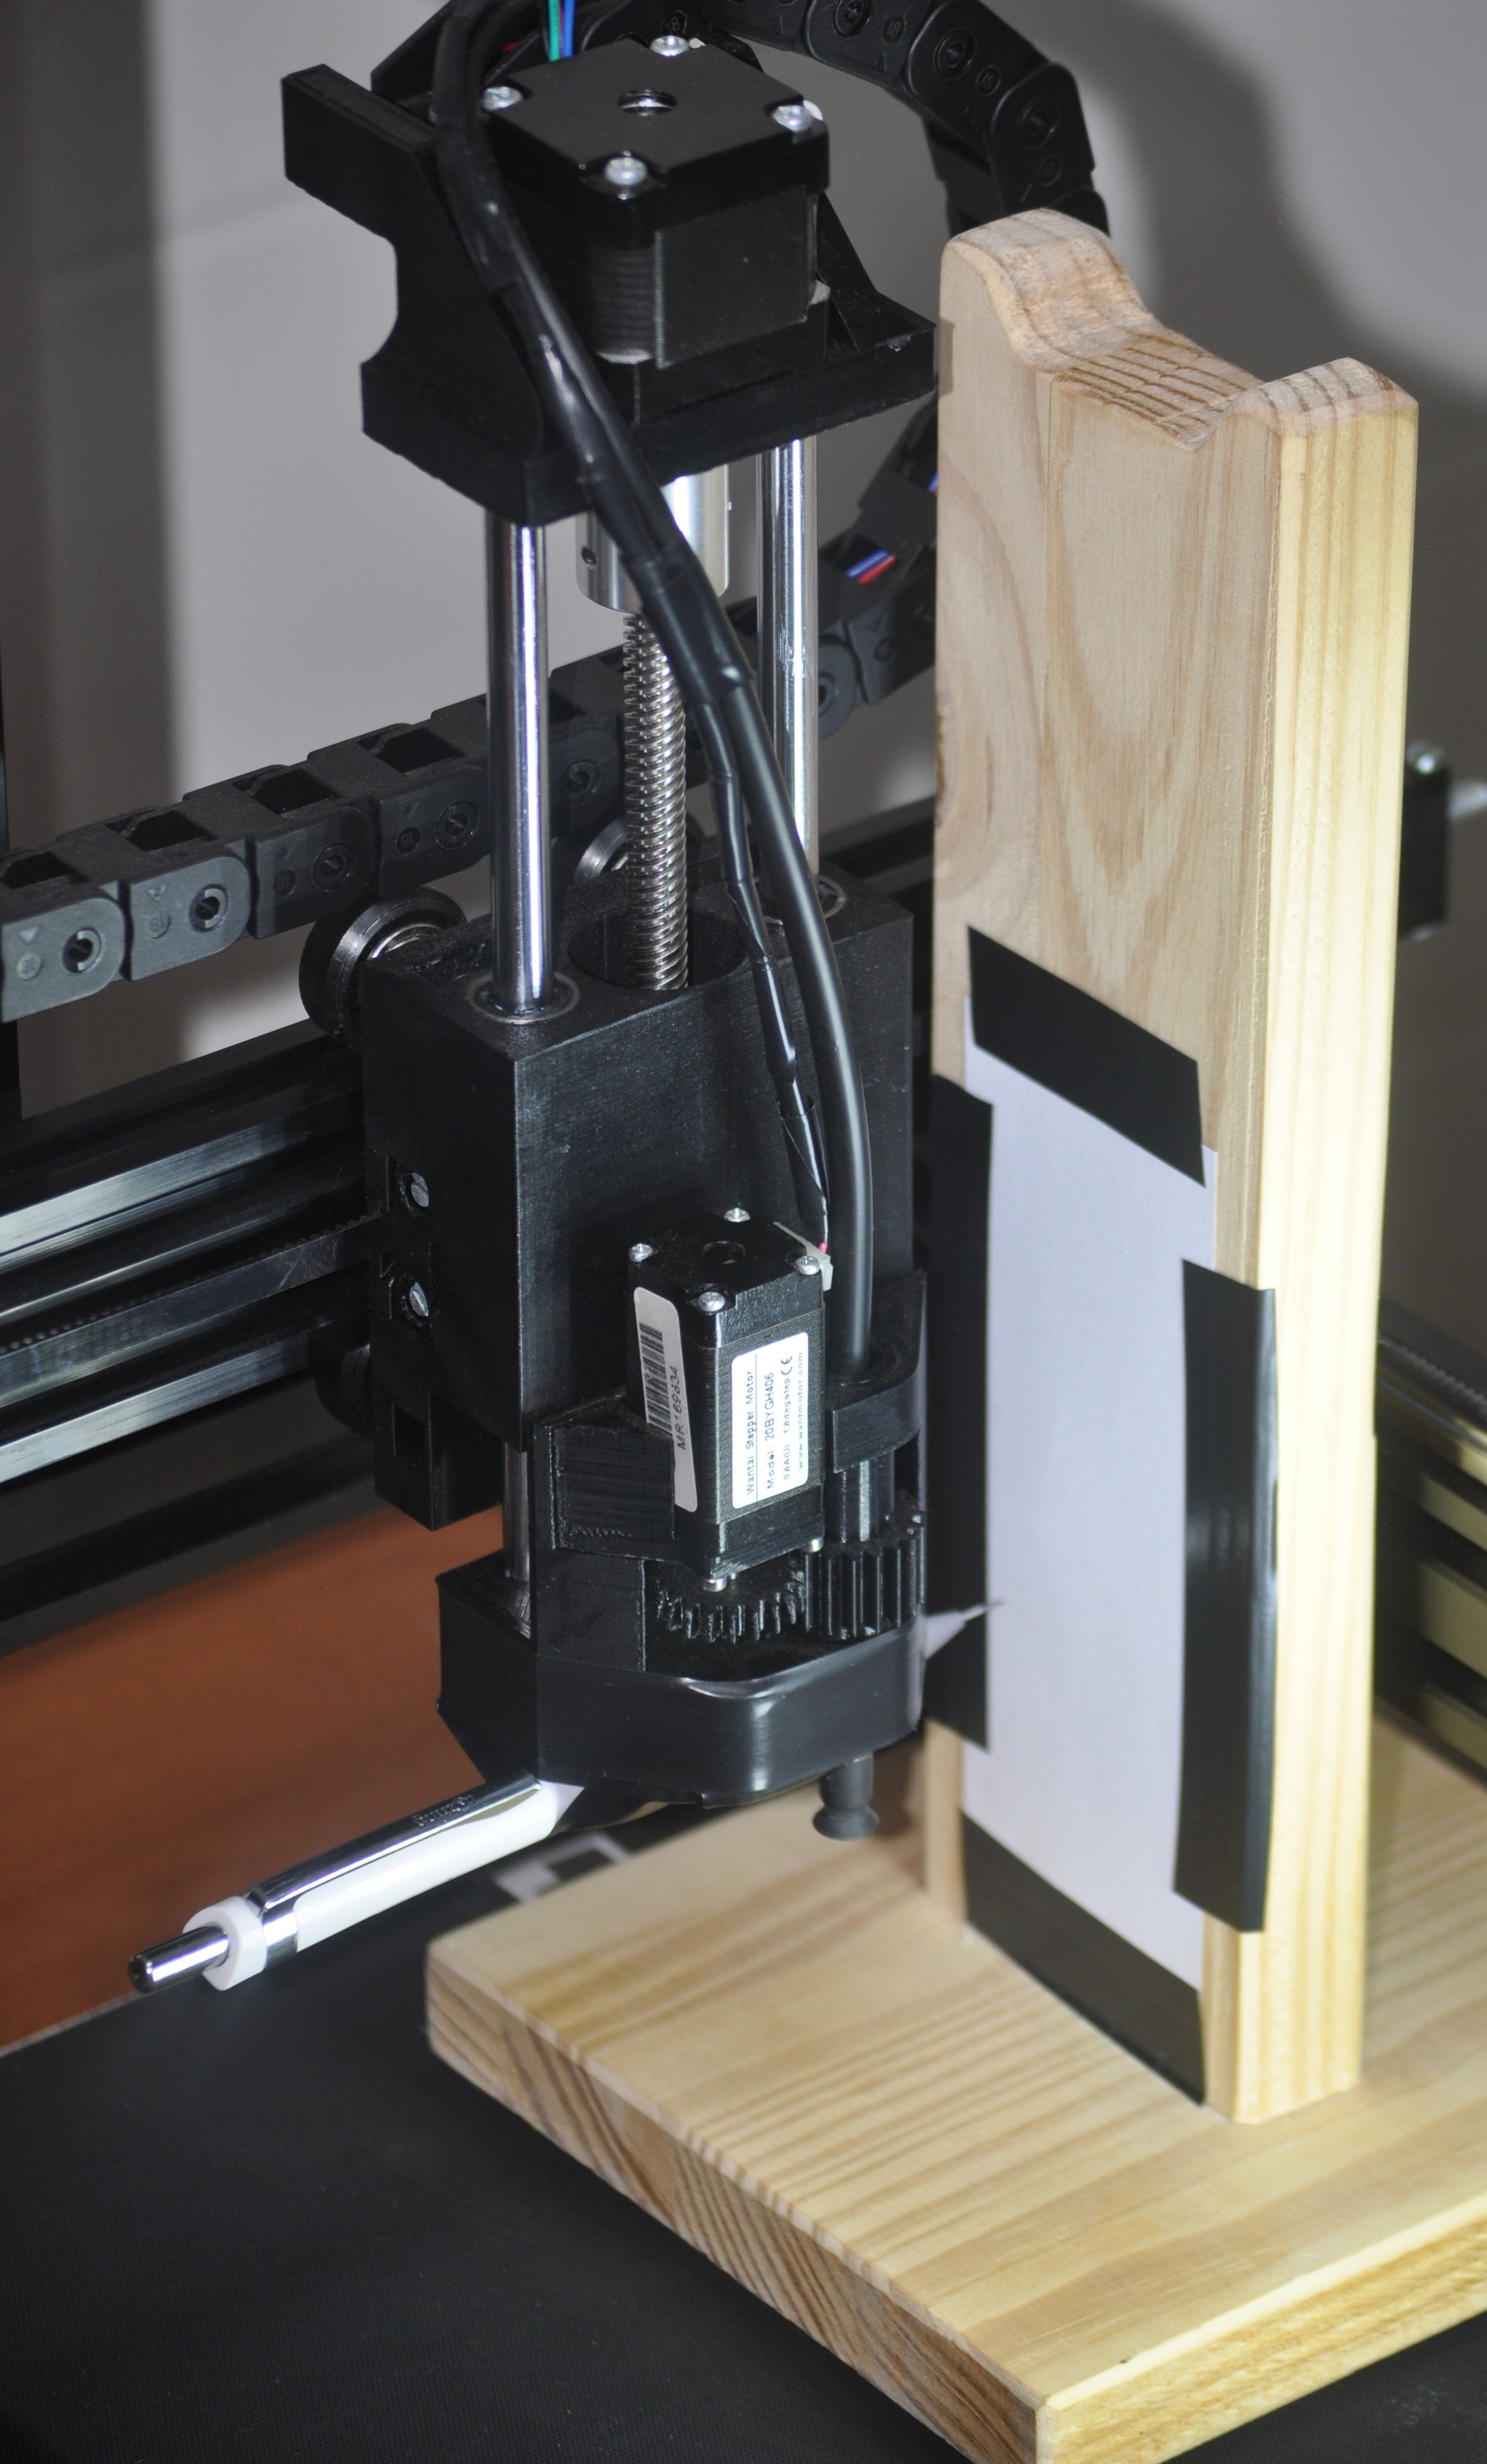
\includegraphics[width=0.95\linewidth]{figures/qualification-test-z-repeat-stand.jpg}
		\caption{Stand setup}
		\label{fig:qtp4-z-axis-test-structure}
	\end{subfigure}
	\caption{Experimental setup configuration used during qualification test 4.}
	\label{fig:qtp4-linear-repeatability-setup}
\end{figure}

\textit{Steps followed in the test or experiment}

The following steps were carried out to execute this qualification test:

\begin{compactenum}
	\item Using the position controls in the system GUI's \textit{Construction} view, iteratively reduce the z-position of the robot until the tip of the mechanical pencil touches the sheet of paper on the base plane firmly enough to leave a mark on the paper. Record this z-position in steps as $z_{mark}$.
	\item Let the x and y coordinates of the position where the robot's repeatability is being tested be denoted by $x_{test}$ and $y_{test}$ respectively. Let the x- and y- coordinates of the reference position to where the robot moves after making a mark be denoted by $x_{ref}$ and $y_{ref}$. Select these values as $x_{test}=0$, $y_{test}=0$, $x_{ref}=1015$ and $y_{ref}=1125$ steps.
	\item Move the robotic end-effector to position ($x_{test}$, $y_{test}$, $z_{mark}$ + 50) where the elements of this tuple refer to the x-, y- and z-position of the robot respectively.
	\item Decrease the z-position of the robotic end-effector to $z_{mark}$ to place a mark on the paper on the base plane.
	\item Increase the z-position of the robotic end-effector to $z_{mark}$ + 50 to remove the pencil tip from the paper.
	\item Move the robotic end-effector to the reference position ($x_{ref}$, $y_{ref}$, 2200) where the state tuple contains the target x-, y- and z-position of the robotic end-effector respectively.
	\item Repeat steps 3 to 6 until a total of 10 iterations have been completed for the given test position.
	\item Repeat steps 2 to 7 with  $x_{test}=1015$, $y_{test}=1125$, $x_{ref}=0$ and $y_{ref}=0$ steps.
	\item Repeat steps 2 to 7 with  $x_{test}=1015$, $y_{test}=0$, $x_{ref}=0$ and $y_{ref}=1125$ steps.
	\item Repeat steps 2 to 7 with  $x_{test}=0$, $y_{test}=0$, $x_{ref}=1015$ and $y_{ref}=0$ steps.
	\item Repeat steps 2 to 7 with  $x_{test}=507$, $y_{test}=562$, $x_{ref}=0$ and $y_{ref}=0$ steps to test the repeatability in the middle of the robot's workspace.
	\item Remove the and reattach the mechanical pencil horizontally and securely to the robot's \textit{End-Effector Assembly} using electrical tape as shown in Figure \ref{fig:qtp4-horizontal-pencil}.
	\item Attach a piece of plain white paper to the vertical surface of the flat-faced stand as shown in Figure \ref{fig:qtp4-z-axis-test-structure} and place the stand in the back right corner of the robot's workspace with the vertical face aligned with the zy plane.
	\item The z-repeatability for two z-planes are tested simultaneously by moving between the two planes and marking a point on the paper for each plane. Let the lower plane be denoted by $z_{lower}$ and the upper plane be denoted by $z_{upper}$. Select these values as $z_{lower}=500$ and $z_{upper}=2300$ steps.
	\item Position the robotic end-effector such that the tip of the mechanical pencil touches the sheet of paper on the vertical stand surface firmly enough to leave a mark on the paper. Record the x- and y-position in steps as $x_{mark}$ and $y_{mark}$ respectively.
	\item Move the robotic end effector to ($x_{mark}$ - \textit{offset}, $y_{mark}$, $z_{lower}$) where \textit{offset}=50 steps when the vertical stand is facing left and \textit{offset}=-50 steps when facing right.
	\item Set the x-position of the robotic end-effector to $x_{mark}$ to mark the point on the paper.
	\item Set the x-position of the robotic end-effector to $x_{mark}$ - \textit{offset} to remove the pencil tip from the paper.
	\item Set the z-position of the robotic end-effector to $z_{upper}$.
	\item Set the x-position of the robotic end-effector to $x_{mark}$ to mark the point on the paper.
	\item Set the x-position of the robotic end-effector to $x_{mark}$ - \textit{offset} to remove the pencil tip from the paper.
	\item Repeat steps 16 to 21 until 10 iterations have been performed.
	\item Repeat steps 15 to 22 with the vertical stand in the back left, front right, front left and centre of the robot's workspace.
	\item For each cluster of point markings on each sheet of paper, set the digital caliper to 2.00 mm and press the tips of the caliper into the sheet of paper near the point such that the paper is indented with the 2.00 mm reference mark.
	\item Take a photo of each cluster of point markings using the digital camera.
	\item Use the ImageJ image processing software to isolate the cluster of point markings.
	\item Using ImageJ, calibrate for length using the 2.00mm reference indents and measure the spread of the markings in the x, y and z directions depending on the sample. Record these measurements.
\end{compactenum}

\textit{Results or measurements}

\ldots

\textit{Observations}

\ldots

\textit{Statistical analysis}

\ldots

\textbf{Qualification Test 5: Measurement of robotic manipulator's rotational accuracy}

\textit{Objectives of the test or experiment}

The aim of this test is to determine the rotational repeatability of the robotic manipulator rotational positioning about the z-axis.

\textit{Equipment used}

The following equipment was used to execute this qualification test:

\begin{compactitem}
	\item PC,
	\item \textit{PC System} software
	\item \textit{Robotic Subsystem},
	\item USB Type A to micro USB connector cable,
	\item an aluminium cube with a side length of 12.6mm $\pm$0.05mm,
	\item 25 x 20 grid of 10mm squares printed on a sheet of white A4 paper,
	\item Digital caliper,
	\item Electrical tape,
	\item and a 30 cm ruler.
\end{compactitem}

\textit{Test setup and experimental parameters}

The following steps were completed in preparation for this qualification test:

\begin{compactenum}
	\item Ensure the \textit{General System Initialisation} procedure has been completed.
	\item Navigate to the \textit{Construction} view in the system control GUI.
	\item Place the grid paper approximately in the centre of the robot's workspace. The grid does not need to be aligned with the robot's coordinate system.
	\item Secure the grid paper in place to the base plane using electrical tape as shown in Figure \ref{fig:qtp5-orientation-grid}.
\end{compactenum}

\begin{figure}[!ht]
	\centering
	\includegraphics[width=0.7\linewidth]{figures/robot-white-grid.jpg}
	\caption{Placement of grid in the robot's workspace to facilitate the measurement of the z-axis rotational repeatability.}
	\label{fig:qtp5-orientation-grid}
\end{figure}

\textit{Steps followed in the test or experiment}

The following steps were carried out to execute this qualification test:

\begin{compactenum}
	\item Choose any one of the 250 mm long grid lines and align the ruler with the line. Press down on the ruler so that the ruler does not shift from this position.
	\item Place the cube on the base plane and use the ruler to align the cube with the 250mm long grid line.
	\item Remove the ruler without disturbing the position or the orientation of the cube.
	\item Use the robot position controls in the \textit{Construction} view of the system control GUI to align the end-effector suction cup with the top of the cube.
	\item Set the rotational step position of the end-effector to 0 steps.
	\item Use the robot position and actuation controls in the \textit{Construction} view of the system control GUI to pick up the cube slightly above the base plane.
	\item Set the robotic end-effector's rotational step position to either 78 steps (odd iterations) or -78 steps (even iterations).
	\item Set the robotic end-effector's rotational step position back to 0 steps.
	\item Use the robot controls to move the cube vertically downwards, place the cube on the base plane and release the cube.
	\item Move the robotic end-effector vertically upwards and to a position that does not restrict access to the robot's workspace.
	\item Press down on the top face of the cube to preserve its orientation and position. 
	\item Use the face nearest to the 250 mm grid line to align the ruler against the cube. Press down on the ruler to preserve the ruler's orientation and position.
	\item Remove the cube from the robot's workspace.
	\item Let the first and last 200 mm long grid lines be denoted by $y_0$ and $y_1$ respectively. Use the placed ruler to draw a line that extends the full length of the grid and intersects with $y_0$ and $y_1$.
	\item Repeat steps to 1 to 14 until a total of 18 iterations have been completed using a different 250 mm grid line in each instance.
	\item Using the digital caliper, measure the deviation of the intersection of for each drawn line with $y_0$ from the intersection of the corresponding 250 mm grid line with $y_0$. Repeat this with $y_1$.
	\item Calculate $\phi$, the angle of each drawn line with respect to the corresponding 250 mm grid line as
	
\begin{equation}
	\phi=\arctan\frac{\delta_0-\delta_1}{\Delta x},
\end{equation}

	where $\delta_0$ and $\delta_1$ are the intersection deviations on $y_0$ and $y_1$ respectively while $\Delta x$ is the length of the 250 mm grid line
	\item Record these results.
\end{compactenum}



\textit{Results or measurements}

\ldots

\textit{Observations}

\ldots

\textit{Statistical analysis}

\ldots

\textbf{Qualification Test 6: Measurement of computer vision cube detection accuracy}

\textit{Objectives of the test or experiment}

The aim of this test is to determine the accuracy of the computer vision system in detecting and localising cubes whose faces are visible from a vertical perspective. Specifically, the test aims to determine the accuracy of the linear localisation along the x-axis and y-axis as well as the rotational pose estimation about the z-axis.

\textit{Equipment used}

The following equipment was used to execute this qualification test:

\begin{compactitem}
	\item PC,
	\item \textit{PC System} software
	\item \textit{Robotic Subsystem},
	\item USB Type A to micro USB connector cable,
	\item Logitech C920 HD Pro Webcam,
	\item 19 Aluminium cubes with side lengths of 12.6mm $\pm$0.05mm,
	\item Mechanical pencil,
	\item Matte black paper,
	\item Electrical tape,
	\item and a 30 cm ruler.
\end{compactitem}

\textit{Test setup and experimental parameters}

The following steps were completed in preparation for this qualification test:

\begin{compactenum}
	\item Place the matte black paper on the base plane of the robot's workspace and secure it in place using the electrical tape.
	\item Navigate to the \textit{Construction} view in the system control GUI.
	\item Move the robotic end-effector to the four extreme points on the base plane of the workspace and mark these point on the black paper using the mechanical pencil.
	\item Draw four lines to join these points to form a rectangle on the black paper using the mechanical pencil and ruler. Using the ruler, mark every 10 mm on each of the four lines.
\end{compactenum}

\textit{Steps followed in the test or experiment}

The following steps were carried out to execute this qualification test:

\begin{compactenum}
	\item Using the 10 mm markings as reference, place the ruler across the robot's workspace at an angle of 0$\degree$ with the x-axis of the robot's coordinate system. Do this at a number of positions. In each instance, press the ruler down firmly to preserve it's orientation and position.
	\item For each ruler placement, place a number of cubes by using the ruler to ensure the angle of each cube with with respect to the x-axis is 0$\degree$. Continue this process until 16 cubes have been placed.
	\item Using the robot position control in the system control GUI, align the suction cup of the robotic end-effector with the centre of the top face of each cube. Record the robotic end-effector's x and y coordinates when aligned with each cube. These are taken as the known world coordinate's of each cube.
	\item Click the \textit{Process Scene} button in the \textit{Construction} view of the GUI to trigger a capture and process action from the \textit{Vision System}.
	\item Record the position and orientation of each cube as estimated by the \textit{Vision System}.
	\item Repeat steps 1 to 5 using a ruler angle of 45 $\degree$ and a total of 19 cubes.
\end{compactenum}

\textit{Results or measurements}

\ldots

\textit{Observations}

\ldots

\textit{Statistical analysis}

\ldots

\textbf{Qualification Test 7: Test of system's capability to detect a dropped cube and and shape construction failure}

\textit{Objectives of the test or experiment}

The aim of this test is to determine if the system is capable of detecting when a cube has been dropped by the end-effector.

\textit{Equipment used}

The following equipment was used to execute this qualification test:

\begin{compactitem}
	\item PC,
	\item \textit{PC System} software
	\item \textit{Robotic Subsystem},
	\item USB Type A to micro USB connector cable,
	\item Logitech C920 HD Pro Webcam,
	\item and 30 Aluminium cubes with side lengths of 12.6mm $\pm$0.05mm.
\end{compactitem}

\textit{Test setup and experimental parameters}

The following steps were completed in preparation for this qualification test:

\begin{compactenum}
	\item Ensure the \textit{General System Initialisation} procedure has been completed.
	\item Navigate to the \textit{Construction} view in the system control GUI.
\end{compactenum}

\textit{Steps followed in the test or experiment}

The following steps were carried out to execute this qualification test:

\begin{compactenum}
	\item Click on the \textit{Load model} button and select the \textit{.cubeworld} an arbitrary 30 cube test shape file.
	\item Clear the \textit{Robotic Subsystem's} workspace and place the 30 cubes at the pre-defined \textit{source cube} locations.
	\item Click on the \textit{Start Construction} button in the system control software to initiate the construction process.
	\item For each of the first 5 cubes, click the \textit{Release Actuator} button in the system control software to force the robot to drop the cube while carrying the cube to the structure.
	\textit Note whether the robot detects the dropped cube condition before in the GUI info log before proceeding with construction.
	\item For cubes 6 to 10, manually remove the cube from the grip of the end-effector during the robot's final downward movement to place the cube and place the cube in the robot's workspace.
	\item Note whether the robot detects the dropped cube condition before in the GUI info log before proceeding with construction.
	\item Repeat steps 5 to 6 with cubes 11 to 15, but remove the cube during the robot's horizontal motion while moving the cube to the structure.
	\item Repeat steps 5 to 6 with cubes 16 to 20, but remove the cube during the robot's upward motion after gripping the cube.
	\item Repeat steps 5 to 6 with cubes 21 to 25, but remove the cube while the robot is moving to grip the cube.
	\item After the 25th cube has been placed, push the structure under construction until at least 1 cube falls from the structure.
	\item Note whether the system detects a construction failure condition using the GUI info log.
	\item Repeat steps 1 to 11 with a different test shape structure until 5 iterations have been completed.
\end{compactenum}

\textit{Results or measurements}

\ldots

\textit{Observations}

\ldots

\textit{Statistical analysis}

\ldots

\newpage

%% End of File.



%%
%%  Department of Electrical, Electronic and Computer Engineering.
%%  EPR400/2 Final Report - Section 5.
%%  Copyright (C) 2011-2021 University of Pretoria.
%%

\section{Discussion}

\subsection{Interpretation of results}

\subsection{Critical evaluation of the design}

\subsection{Design ergonomics}

\subsection{Health, safety and environmental impact}

\subsection{Social and legal impact of the design}

%% Potential improvements
%% - Used an improved approach to solve the PnP and estimate the extrinsic matrix

\newpage

%% End of File.



%%
%%  Department of Electrical, Electronic and Computer Engineering.
%%  EPR400/2 Final Report - Section 6.
%%  Copyright (C) 2011-2021 University of Pretoria.
%%

\section{Conclusion}

\subsection{Summary of the work completed}

This report details the work that was performed during the design and development of a robotic system with the overarching goal of constructing arbitrary 3d shapes using small construction cubes.

A literature study was undertaken into computer vision approaches to object detection, with a focus on traditional techniques, as well 3D object localisation methods and their application to the robotics domain. Firstly, a gantry robot was designed from first principles and manufactured using a combination of 3D printing and metal machining technologies. Following this, the hardware of embedded robot control circuit was designed from first principles and a prototype was created on a breadboard. The software was implemented on the embedded controller using C. A PCB was designed for the circuit and sent for manufacturing overseas.

A 3D render based GUI was developed using a low-level graphics API to facilitate the definition of 3D shapes. A computer vision system was developed to detect and localise the cubes within the robot's workspace. Finally, PC-based software was developed to integrate the shape definition GUI and computer vision components as well as to control the robot. A number of test shapes were defined using the shape definition GUI and constructed closed loop by the gantry robot supported by the computer vision system.

\subsection{Summary of the observations and findings}

The system developed, which had a PC-based software component and a robotic system as its primary two constituents, was successful in fulfilling the overarching goal of constructing arbitrary 3D shapes using small construction cubes. The system was capable of constructing all test shapes that met the minimum specifications of containing 30 cubes with at least four cubes in height. In addition, the system was capable of constructing shapes up to six cubes in height that contained arbitrary cube rotations about the z-axis, partially supported cubes, small inter-cube tolerances and leaning cube stacks.

The system was able to perform the construction closed loop by using the computer vision system to assist in handling unexpected events. Specifically, the system was able to successfully detect, re-grip and re-orient the cube in the dropped cube case and issue a construction failure signal in the structural damage case. A gantry robot approach with a design focus on the rigidity of the mechanical component was found to be a successful approach to the cube construction task. Furthermore, the pin-hole camera model based approach to 3D cube localisation component of the through mapping image coordinate system to the world coordinate system was found to be a robust solution for the computer vision component of this task.

\subsection{Contribution}

The domain of mechanical design for robots and the construction needed to be explored to complete this project. In particular, the domain of CAD software, and specifically the Fusion 360 CAD software package, needed to be mastered to assist in the creation of the mechanical component of the \textit{Robotic System}. Furthermore, an understanding of the functionality and applicability of a number of mechanical components, including linear drive and linear motion systems, needed to be acquired. In particular, this included the integration and control of servo and stepper motors. The mechanical construction required the attainment of knowledge to facilitate the direct use of a 3D printer as well as metal machining tools such as a lathe and milling machine. All of the aforementioned components are common in a Mechanical Engineering undergraduate course but are all non-existent in a Computer Engineering undergraduate course. The study leader provided helpful guidance in terms of highlighting the challenging aspects of the mechanical design which should be focused on as well as favorable characteristics that should form part of the design.

A combination of new theory and the approaches arising from this theory needed to be mastered in the computer vision domain. Specifically, traditional computer vision techniques used for object detection needed to be understood and implemented as well as 3D localisation approaches. In service of the latter aspect, knowledge of the pin-hole camera model needed to be acquired and used in mapping between the image coordinate system and world coordinate system. This approach followed from the study leader's suggestion to use and explanation of camera intrinsics and extrinsics. Furthermore, knowledge of the computer vision library OpenCV was acquired to support the computer vision system development at various stages. None of this computer vision knowledge is covered by undergraduate modules. 

In a number of undergraduate modules, first principles 8-bit microcontroller development and 32-bit microcontroller development boards with hardware abstraction libraries were explored. The first principles development of embedded software for a 32-bit microcontroller as well s the complete first principles design of the controller circuit required the attainment of new knowledge. Furthermore, the development of a PCB for the controller required the PCB design software KiCAD to be mastered. Lastly, for the shape definition component, new knowledge about the theory relating to the graphics pipeline and transformation matrices used in 3D graphics rendering needed to be acquired. The use of the low-level graphics API OpenGL needed to be understood for this purpose.

There were no novel software algorithms or hardware circuits developed in this project. However, the design of the mechanical component of the \textit{Robotic System}, the hardware of the embedded controller circuit, the embedded software, the 3D rendering software, the computer vision software and system controller was completely from first principles which resulted in unique designs and implementations for each of these facets. During the course of the development of these components, the study leader highlighted the challenging facets of each which should receive the requisite attention.

Libraries were relied on heavily during the initial design and prototyping phase for the computer vision system and embedded controller. The embedded controller implementation was converted completely to a first principles implementation. The core aspects of the computer vision system were developed from first principles while basic image processing functions were retained from the OpenCV library. The calibration aspects of the computer vision component were also considered as not a core aspect of the computer vision system and OpenCV was used for this purpose. Lastly, the high-level idea for the approach to the custom square corner detection algorithm was inspired by a student in the same research group in their approach to detecting puzzle-piece corners. However, the design and implementation of this algorithm was from first principles and only loosely related. 

\subsection{Future work}

The success of the design of the robotic subsystem provides a solid foundation for further development going forward. The first aspect the should be investigated further is the improvement of the cube localisation accuracy of the computer vision system to improve the tolerance used for shapes constructed in a closed loop manner. Secondly, the use of a stereo vision computer vision approach or an ToF camera over the monocular vision approach used in this project are possible future avenues of exploration that would eliminate the need to assume the z-plane in which a cube is detected. In addition, relatively simplistic path planning approaches were used in this project. Therefore, a possible avenue of improvement would involve an investigation into the use of more sophisticated path planning approaches. 

For a given construction sequence, the cubes are made available to the robot by placing the cubes in pre-defined locations. An alternative approach that should be explored involves the arbitrary initial placement of the cubes within the robot's workspace followed by the implementation of an algorithm that would allow the robot to detect the cubes and construct the shape from this initial state. Finally, on a related note, it was observed that one of the main sources of inaccuracy in the system was the deviations introduced when the robot gripped the \textit{source cube} for construction. Therefore, further work into improving the accuracy of the \textit{source cube} attainment mechanism should be done.

\newpage

%% End of File.




%% Use the IEEE Transactions style for the references.
\bibliographystyle{IEEEtran}
\bibliography{finalreport}
\newpage

%% --- PART 4 ------------------------------------------------------------

\eprsec{Part 4. Appendix: technical documentation}
\newpage

\setcounter{secnumdepth}{0}

\titleformat{\subsection}[display]
{\fontsize{14pt}{16.8pt}\selectfont\bfseries} {} {5pt} {\formatsubsectiontitle}
\titleformat{\subsection}[display]
{\fontsize{14pt}{16.8pt}\selectfont\bfseries} {} {5pt} {\formatsubsectiontitle}

%%
%%  Department of Electrical, Electronic and Computer Engineering.
%%  EPR400/2 Final Report - Technical Documentation.
%%  Copyright (C) 2011-2021 University of Pretoria.
%%

\section{HARDWARE part of the project}

\subsection{Record 1. System block diagram}


\subsection{Record 2.  Systems level description of the design}


\subsection{Record 3. Complete circuit diagrams and description}


\subsection{Record 4. Hardware acceptance test procedure}


\subsection{Record 5. User guide}


%% --------------------------------------------------------------------

\section{SOFTWARE part of the project}

\subsection{Record 6. Software process flow diagrams}


\subsection{Record 7. Explanation of software modules}


\subsection{Record 8. Complete source code}
Complete code has been submitted separately on the AMS.


\subsection{Record 9. Software acceptance test procedure}


\subsection{Record 10. Software user guide}


%% --------------------------------------------------------------------

\section{EXPERIMENTAL DATA}

\subsection{Record 11. Experimental data}


%% End of File.




\end{document}

%% End of File.
